\documentclass[10pt,oneside,a4paper,onecolumn,titlepage,draft]{lancsthesis}
% =============================================================================

\usepackage{lancsthesis}    % Book format, local copy
\usepackage{swLaTeXTools}   % Custom additions and commands

% UTF-encoded input files
\usepackage[utf8]{inputenc}

% Allow insertion of outline
\usepackage{pdfpages}

% Change the way footnotes are numbered.
\usepackage{chngcntr}
\counterwithout{footnote}{chapter}

% \text and more in math mode
\usepackage{amsmath}

% Page refs in the bibliography
% \usepackage{backref}

% Merging table cells.
\usepackage{multirow}

% Remove me after drafting
\usepackage{ifdraft}


% Line spacing needed for lancsthesis
\usepackage{setspace}
\linespread{1.45}    % double spacing is 1.6, half is 1.3
% \onehalfspacing
% \doublespacing


% Code Listings
\usepackage[final]{listings}
\lstset{breaklines=true}
\lstset{numbers=left}
\lstset{captionpos=b}
\lstset{extendedchars=true}
% \lstset{basicstyle=\linespread{1}}

% Font: URW Palladio (Palatino clone)
\usepackage{pxfonts}
\usepackage[T1]{fontenc}

% Dropcaps
% \usepackage{lettrine}
% \newcommand{\dropcap}[2]{\lettrine[lraise=0.2,nindent=0.2em,slope=-.5em]{#1}{#2}}

% Ability to include PDFs
\usepackage{pdfpages}

% configure graphics
\setkeys{Gin}{draft=false}  % Graphics show in draft mode
\usepackage{graphicx}
\graphicspath{{./images/}}
\DeclareGraphicsExtensions{.pdf,.png,.jpg,.eps}

% Rotation of some figures and tables
\usepackage{rotating}

% Multi-page tables
% Used in tex/persona/results.tex only, commented out there.
% \usepackage{longtable}

% Two-column spanned tables
% \usepackage{supertabular}

% Two column blocks
% \usepackage{multicol}

% Subliminal text position hints
% Requires PdfTeX, XeTeX or LuaTeX
\usepackage{microtype}

% Restrictions on figure movement
\usepackage{placeins}

% Hyperlinks back from the bibliography to the use
% \usepackage{backref}

% hyperref (should be last)
\usepackage{hyperref}
\hypersetup{%
    final=true,     % Show even when doc is in draft mode
    hidelinks=true,
    unicode=true,   % Enable the 21st century
    pdfborder={0,0,0,[]},
    pdfauthor={Stephen Wattam},
    linkbordercolor={0 0 0},
    citebordercolor={0 0 0},
    urlbordercolor={0 0 0},
    urlcolor=blue,
    filecolor=black,
    citecolor=red,
    linkcolor=black,
    colorlinks=true,
    bookmarks=true,
    linktocpage=true,
    linktoc=all
}%


% ------------------------------------------------------------------------------
%  Drafting 
% ------------------------------------------------------------------------------
%
% Watermark if in draft mode
\ifdraft{%
    \usepackage{draftwatermark}
    \SetWatermarkScale{1.5}
    \SetWatermarkLightness{0.95}
}{}

% Page layout (margins)
\ifdraft{%
    % inline layout
    \usepackage[left=38mm,top=25mm,right=38mm,bottom=25mm]{geometry}

    \usepackage{todonotes}
    \newcommand{\td}[1]{\todo[fancyline,size=\tiny,color=yellow!20]{#1}}
    \newcommand{\til}[1]{\todo[inline,size=\small,color=yellow!20]{#1}}
}{% else
    % book layout (asymmetric)
    \usepackage[left=38mm,top=25mm,right=25mm,bottom=25mm]{geometry}
    
    \newcommand{\td}[1]{}
    \newcommand{\til}[1]{}
}%

% ------------------------------------------------------------------------------





% =============================================================================
%  Begin document
% =============================================================================
\begin{document}
\frontmatter
% \thispagestyle{empty}



% =============================================================================
%  Title Page
% =============================================================================
%% TODO: port this to the lancsthesis.cls style as \title
\begin{center}
\begin{tabular}{c}
\vspace{2in}\\
\begin{minipage}{5in}
\begin{center}
{\bf \huge 

	
Big Scary Thesis Title:\\


Powered by Tea and delusion\\
%{\small `tea' is capitalised because it fucking rocks.}
% TODO

}
\vspace{2in}


{\bf \Large Stephen Wattam}

\vspace{2in}


Submitted for the degree of Doctor of Philosophy\\
at Lancaster University, \\
January 1901.
% TODO

\end{center}
\end{minipage}
\end{tabular}
\end{center}
\newpage






% =============================================================================
%  Introductory items
% =============================================================================
\chapter*{Abstract}
Current efforts in corpus linguistics and NLP centre around the use of corpora---large language samples that are intended to describe a whole population of language users.

% Historically these items have had their utility abrogated by a number of economic, social and practical limitations.

Perhaps because of the hard-won nature of the first corpora, many characteristics of their design have proven intransigent.  This yields many benefits for science---many studies are comparable and interaction between those in the field is simplified, however, many corpus-building efforts serve to replicate these older designs, rather than adapting them to suit available technological innovations.

The rise of web as corpus (WaC), and more recently big data, has provided us with the tools needed to build corpora with very little supervision.  This allows us to re-examine and, in places, exceed the limitations of conventional corpora.  Even so, many corpora are compared against conventional ones due to their status as a de-facto gold standard of representativeness.

Though the processes involved in building web corpora introduce their own limitations, this ease of access allows for improved adherence to the theoretical ideals of sampling, and thus a complementary strategy for corpus design.

%---

In this thesis I'll provide justification for the development of new sampling procedures guided less by concepts of linguistic balance, intuition and coverage, and more by statistical sampling theory.  I apply these methods to the problem of improving WaC samples (whilst avoiding their novel pitfalls), and present ways in which the whole scientific process of corpus comparison, dissemination and replicability may be assessed---itself something that demands an alternative view of corpus goals.  I go on to present tools that make these tasks easy to apply in a scientific context, in order to construct usable and practical web-derived corpora.



%\pagebreak


\ifdraft{%
    \chapter*{Acknowledgements}
    
This thesis could not have been completed without the support of many people.  Through the considerable time it took, many academics and friends have helped answer my questions and allay (or confirm!) my fears.  My thanks go out to all members of UCREL, who taught me the ways of the corpus.

Foremost amongst these must be my supervisors, Paul Rayson and Damon Berridge.  Their direction and encouragement was often the only thing keeping me in the office, and it is hard to overstate their influence.

Secondly, my friends, particularly Carl Ellis, Matthew Edwards, John Vidler and John Hardy.  Our (sometimes not so) implicit competition has been endlessly motivating, even thought I seldom won.

Finally, I wish to thank my parents.  It is doubtless my mother's lesson to question the world that has lead me into research, and my father's work ethic (however diluted during inheritance) that has carried me this far.

\begin{center}
Thank you all.
\end{center}




}{}
%\pagebreak

\chapter*{Declaration}
%TODO
Declaration

% space for signature
\vspace{2in}
\dotfill SW 


% space for supervisor's signature
\vspace{1in}
\dotfill PR 


%% space for supervisor's signature
%\vspace{1in}
%\dotfill DB 

%\pagebreak

% Auxiliary introductory things
\tableofcontents
\listoffigures
\listoftables
\clearpage



% =============================================================================
%  Start of Actual Content
% =============================================================================
\mainmatter


\chapter{Introduction}
\label{sec:introduction}

The evaluation of corpus construction is a particularly tricky area: without a gold standard or real-world task to frame the results, it is often difficult to tell quantitatively what differences between corpora constitute improvements.


The way seed-based methods work offers an ideal source of gold standard data, nonetheless, only experience and repeated use can reveal the manner of the differences identified, and its impact on experimental results.  This evaluation will use this reflexive method to identify overall responsiveness to the seed corpus, along with an examination of individual components of the system as a method for revealing specific strengths and weaknesses.

This evaluation is based around one of tasks identified in Chapter~\ref{sec:rebuilding}---that of rebuilding a corpus from scratch based upon a seed's proportions.  This task is effectively a super-task of reconstructing or repairing a corpus, and is equivalent to many scenarios involving disseminating sensitive corpora with minor restrictions on the metadata dimensions used.



This chapter begins with a description of the use cases covered, and a detailed rationale of how these form testable, objective research questions.

Section~\ref{sec:evaluation:rqs} details the two main approaches to evaluation: those applied to individual components, and those applied to the results of running the implementation as a whole.

Following that, each stage of the corpus building process is evaluated in a white-box fashion, starting with the heuristics used to classify documents (Section~\ref{sec:evaluation:heuristics}) and moving on to the process of identifying `target' prototype documents in vector space (Section~\ref{sec:evaluation:resampler}), and then retrieving documents from the web itself (Section~\ref{sec:evaluation:retrieval}).

Finally, the implications of each component's functionality to the final process, and what the results tell us about the state of the web as a document source for resampling BNC-like corpora, are discussed in Section~\ref{sec:evaluation:discussion}.








\chapter{Background}
\label{sec:litreview}
Large samples of text, known as corpora, are fundamental to a great number of users.  The groups I will be focusing on for the purposes of this thesis are particularly interested in scientific samples, that is, in generalising findings from the corpus to a wider population.  This includes much work in NLP and corpus linguistics, and some of what is commonly termed `data science'\footnote{Though in most `data science' contexts, sampling is performed as an intrinsic part of the task}.


The problem of sampling linguistic data is a well-researched one in the field of corpus linguistics, and a review of linguistics' approach to corpus construction will form the bulk of this review.  This portion of the review begins with a historical overview of approaches to corpus construction, before focusing on the problem of defining a corpus in concrete enough terms to suit the rest of the work presented in the thesis.  It then focuses on potential threats to validity exposed by these methods, both from the point of view of corpus construction and use.

% Not to be neglected, however, is the perspective offered by more formal survey sampling, especially as its use across the social sciences can offer insights into solutions for practical problems.  Each area of sampling is approached as if applied to corpus construction, and its relative concepts identified.

Finally, in~\ref{sec:litreview:newtech} the first few steps towards improving sampling methodology within corpus linguistics are reviewed, with a focus on web-based corpus construction methods.




\section{Corpora and Corpus Linguistics}
\label{sec:litreview:corpora}


The field of linguistics is one concerned with description and formalisation of a particularly ethereal social concept.  The paucity of philosophical agreement upon the nature of language has led to many different approaches being taken through the years, many of which have accomplished great things in advancing our capacity to reason about, and derive conclusions from, language.


The most obvious method for inquiring about the nature of language is to sample real-world use.  This process is followed in many other sciences concerned with social phenomena, and offers a tried-and-tested methodology for inferring results.  It is perhaps unsurprising, then, that this method has been used to a varying degree by many linguists throughout history.

In their 2001 book\cite{macenery2001corpus}, McEnery and Wilson characterise the pre-Chomskian linguistic inquiry as primarily taking this form:

% page 2
\begin{quote}
The dominant methodological approach to linguistics immediately prior to Chomsky was based upon observed language use.
\end{quote}

They point to a number of studies using systematic analysis of samples to make their conclusions\cite{kaeding1897haufigkeitsworterbuch,preyer1889mind,stern1924psychology,eaton1940semantic,west1953general}, and decribe Chomsky's influences on the field, which served to lead it to all but abandon corpus techniques in the 1950's, as a turn towards explanatory, rationalist theories of language.

These rationalist theories were often verified using experimentation or elicitation, in an effort to gather data that is detailed and reliable.  It's arguable just how valid and philosophically defensible these methods are, especially given the nature of language as a part-mental, part-tangible concept.

% These early corpora are of a quite different form to those of the `modern era', and will not be discussed in any great detail here except for historical context.


In a pre-digital world, collection and analysis of large-enough-to-be-useful samples of language was extremely difficult, making this rationalist approach a viable alternative.
Small samples are fundamentally unable to reveal some of the details examined by the structuralists, and construction and analysis of sufficiently large corpora in a non-digital era would prove a practical hard limit on the power of corpus studies.  To frame the focus on rationalist inquiry as an alternative to the empirical is a disservice to both: empiricism had supported the rationalist theories of the 50's, and would itself go on to be supported in turn as it once again rose to prominence.

The revival of corpus linguistics may be attributed almost solely to the availability of programmable computing machinery.  This offered a solution to the problems of scale encountered during earlier corpus analyses, making empirical data once more viable for detailed inspection of language.

This revival, often termed the `modern era' of corpus linguistics, has yielded what we would commonly call a corpus today: a large, machine-readable, annotated collection of texts sampled in order to represent some population of real-world language use.

Corpus studies are now widely relied upon across linguistics, and are often the method chosen to test theories derived from structuralist approaches.  This may be seen as a validation of their methods, as the two complementary philosophies of scientific inference are once more able to use one another without methodological suspicion.

For the purposes of this section I will be focusing on the design of `modern' corpora with respect to their use in validating linguistic theories, and for training automated Natural Language Processing (NLP) and Information Retrieval (IR) systems.  For this reason I will be covering mainly general purpose corpora: those that purport to represent such a large population as to cover a whole language.  This type of corpus is built so as to be useful to many research questions and researchers, in part to dilute practical issues surrounding sampling.  This is in contrast to special-purpose corpus, which are designed to represent a restricted context.  Special-purpose corpora may be selected according to demographic or linguistic properties, and are typically much smaller.  Because of this they are often built for a given study, or by re-sampling a general-purpose corpus.




\subsection{A Brief History of Modern Corpora}
The Brown Corpus of Standard American English\cite{francis1961brown}% http://icame.uib.no/brown/bcm.html
is widely regarded as the first of the modern age of corpora.  Built in the 60's, Brown's corpus was the first electronic-format general purpose corpus and was roughly one megaword in size.  % 1,014,312
It contains 500 samples, each comprising roughly $2,000$ words, that were taken to represent a cross-section of works published in the United States in 1961.  The proportions and sizes of samples were selected in order to trade off pragmatic concerns with the possible kinds of analysis that could be performed at the time.

The `Standard' in its name referred to Kucera and Francis' intent that the corpus represents their judgement of `standard' English use.  Brown became a \textsl{de facto} standard for American English, and the design was carried forward into many other corpora, mostly regional versions designed to be comparable to Brown\cite{hundt1999manual,johansson1986tagged,hundt1998manual,shastri1988kolhapur,collins1988australian,bauer1993manual,mcenery2004lancaster}.  In order to maximise the value of comparisons within studies, other general purpose corpora chose to mirror Brown's sampling policies.

% --- 

\begin{table}[Ht]
    \centering

    \begin{tabular}{llrr}
    \hline
    Categories & Texts in each category & American corpus & British corpus \\ \hline
    A & Press: reportage & 44 & 44 \\
    B & Press: editorial & 27 & 27 \\
    C & Press: reviews & 17 & 17 \\
    D & Religion & 17 & 17 \\
    E & Skills, trades, and hobbies & 36 & 38 \\
    F & Popular lore & 48 & 44 \\
    G & Belles lettres, biography, essays & 75 & 77 \\
    H & Miscellaneous & 30 & 30 \\
    J & Learned and scientific writings & 80 & 80 \\
    K & General fiction & 29 & 29 \\
    L & Mystery and detective fiction & 24 & 24 \\
    M & Science fiction & 6 & 6 \\
    N & Adventure and western fiction & 29 & 29 \\
    P & Romance and love story & 29 & 29 \\
    R & Humour & 9 & 9 \\ \hline
      & Total & 500 & 500 \\ \hline
    \end{tabular}

    \caption{The basic composition of the British and American corpora}
    \label{table:litreview:corpora:lobdist}
\end{table}


The Lancaster-Oslo-Bergen (LOB) corpus\cite{johansson1986tagged} was built as a British counterpart to Brown.  
It uses the same stratification and sampling strategy (with one or two more texts in certain categories) and thus comprises roughly a megaword of British English, as published in 1961.  % See  http://clu.uni.no/icame/manuals/ Table 1 for a table of comparisons
Though the manual does note:

\begin{quote}
    The matching between the two corpora is in terms of the general categories only. There is obviously no one-to-one correspondence between samples, although the general arrangement of subcategories has been followed wherever possible.
\end{quote}

Table~\ref{table:litreview:corpora:lobdist} shows the proportions of texts in each genre, relative to Brown (the `American corpus'), as reproduced from the corpus manual.

% ---
The London-Lund Corpus\cite{greenbaum1990london} was released in 1990, and contains transcribed spoken text, annotated with a number of different markers to indicate intonation, timing and other extra-textual information.  
The corpus consists of $100$ texts, each of $5,000$ words, totalling $500,000$ running words of spoken British English.
The annotation scheme used in LLC is much more in-depth than that in many written corpora, reflecting the different nature of research questions for speech.



% --- 
Collins' requirement for a corpus upon which to base their dictionaries spawned the COBUILD and its `representative' subset, the Bank of English\cite{Jarvinen1994AMW991886.991985,sinclair1987looking}.  COBUILD uses a slightly different approach to corpus building: that of the monitor corpus.  Monitor corpora are continually added to, using a fixed sampling policy but an ongoing sampling process.  At the time of writing, the BoE is 650 million words in size (The whole COBUILD family used by Collins is 4.5 billion)\cite{collinswebcorpus}.

The approach taken by the BoE opens many possibilities for analysis of language over time (something also covered by diachronic/historical corpora using more conventional sampling).  Even so, such comparisons are complicated by the irregular additions (c.f.\ diachronic corpora, which contain complete samples for each time), and this remains the only major corpus built in this fashion prior to automated web retrieval.


% ---





The de-facto standard of the day is currently the British National Corpus, which comprises $100$ million words of British English\cite{leech1993100}.  The BNC's design was influenced heavily by discussions on corpus building that centred around creating a standard, reliable approach to taxonomy, sampling and annotation that occurred around the early nineties.

The BNC aims at being a synchronic `snapshot' of British English in the early 1990s.  It consists of samples of text up to $45,000$ words each, and is deliberately general-purpose, containing a wide range of genres as well as a sizable spoken portion.  It was released in 1994, but has since been re-coded and augmented, particularly notably by Lee\cite{lee2003bnc}, who constructed a significantly more detailed (and principled) taxonomy for its texts in 2003.

Lee's genre taxonomy is outlined in Appendix~\ref{sec:appx:sample}.  Lee's decisions to code genres using this system were partially based on fostering compatibility with the ICE-GB\cite{greenbaum1996international} and LOB\cite{johansson1986tagged} corpora.

The prominence and `whole population' coverage of the BNC's sampling frame spawned many compatible corpora, though these often show more variation in sample design than the Brown clones.  Xiao, in his survey of influential corpora, notes the existence of national reference corpora for American, Polish, Czech, Hungarian, Russian, Hellenic, German, Slovak, Chinese, Croation, Irish, Norwegian, Kurdish, and many more\cite{xiaoz2008}.  An updated version, BNC2014\cite{cambridgeuniversitypress2014}, is currently being constructed.

% 1.2 General definitions ( from http://www.natcorp.ox.ac.uk/docs/URG/BNCdes.html )
% 
% The British National Corpus is:
% a sample corpus: composed of text samples generally no longer than 45,000 words.
% a synchronic corpus: the corpus includes imaginative texts from 1960, informative texts from 1975.
% a general corpus: not specifically restricted to any particular subject field, register or genre.
% a monolingual British English corpus: it comprises text samples which are substantially the product of speakers of British English.
% a mixed corpus: it contains examples of both spoken and written language.


% ---
The rise of electronic communications has led to a reduction in the effort required to gather corpus data.  This has resulted in a great increase in the number of special-purpose corpora built for specific studies\cite{westlabusenet2013,baroni2006building,Mair20060101T00000009215034355}.  These corpora are more focused in that their construction methods restrict them to electronic data, yet  their large sample size may make them suitable for the study of smaller-scale features in a more general context.


% Move? [These corpora are often less widely used, and serve to illustrate one extreme discussed below, that the purpose of a corpus is important to its construction]

This thesis is focused on sampling using automated, technical mechanisms to overcome some of the challenges facing conventional methods, and as such focuses on web-based methods (known as `Web as Corpus').  WaC is concerned with sampling the web itself, as well as constructing samples that are representative of other data, yet are retrieved primarily from the web.  This approach, and those using similar methods, are covered below in Section~\ref{sec:litreview:newtech}.






















% ---------------------------------------------------
\subsection{What Makes a Corpus?}
The use of general purpose corpora as large monoliths, reused in many studies and systems, has led to much debate over the nature of a corpus.  This, as we shall see throughout the thesis, is a question unworthy of concrete answers---each purpose will exert certain demands upon corpus design criteria, and any widely-used corpus is likely to be a compromise around these.

This section exists primarily to define the term `corpus' as used here: it is unlikely that the definition derived below is universal, however, it is designed to reflect most use-cases, across corpus linguistics and NLP.

% This discussion is separated to cover a number of properties of corpora, and their parameters.  These 



In order to establish the important traits of corpora, it is wise to have an understanding of the motivation behind their existence.  Corpus methods are generally contrasted against two other methods of linguistic investigation: direct elicitation from a language speaker, and directed research into a linguistic feature under controlled conditions.  Both of these pose significant scientific challenges---both are reliant on at least one linguist's intuitive view of language (one that could hardly be said to be representative of most language users), and both require the acquisition of data without its usual context, something that is especially difficult given the varied and context-dependent complexity of language.

Corpora provide limited solutions to both of these issues.  In the former case, they provide an objective record of linguistic data that is free from all but the initial builders' influences (which, in the ideal case, may be documented and provided along with the data itself).  In the latter, they are as portable as any large volume of text, and may be annotated with context sufficient for a given linguistic task.


%------
At its most basic level a corpus is a sample of text.  Given research questions surrounding a body of text, it is perhaps necessary only to stipulate that a corpus must be represent known population~\cite[p. 22]{mcenery2001corpus}:

\begin{quote}
\ldots{}a body of text which is carefully sampled to be maximally representative of a language or language variety.
\end{quote}

Further to this, the modern definition of a corpus has undergone a series of significant refinements thanks largely to the increase in both the ubiquity and power of computing machinery.  General-purpose corpora are, with very few exceptions, electronic (with an increasing number documenting texts of electronic origin), multi-modal (covering a wide variety of methods of communication and their linguistic features), and annotated with linguistic data.

Many authors go further by stating that a corpus should be machine-readable, annotated with information useful to linguistic inquiry, built for a specific purpose or methodology, available for use in other studies, finite in size or stratified to provide multiple possible analysis methods with internally valid data\cite{bennett2010using,bowker2002working,leech1992corpora}.
%The majority of present-day corpora are “balanced” or “systematic”. This means that the texts are collected (“compiled”) according to specific principles, such as different genres, registers or styles of English (e.g. written or spoken English, newspaper editorials or technical writing); these sampling principles do not follow language-internal but language-external criteria. For example, the texts for a corpus are not selected because of their high number of relative clauses but because
Whilst I do not consider many of these to be requirements for a scientifically useful corpus, they may contribute greatly to corpus utility due to their alignment with common methodologies and uses.  There is undoubtedly a case for this---the utility of a corpus is often limited by its format, however, the extent to which this applies varies wildly by purpose makes it unreasonable to include many resources missing some of the above under the term `corpus'.


%Awesome quote from http://www.linguistics.ucsb.edu/faculty/stgries/research/2009_STG_CorpLing_LangLingCompass.pdf
%However,
%since corpus data only provide distributional information in the sense mentioned earlier,
%this also means that corpus data must be evaluated with tools that have been designed to
%deal with distributional information and the discipline that provides such tools is statistics.
%And this is actually completely natural: psychologists and psycholinguists undergo comprehensive
%training in experimental methods and the statistical tools relevant to these methods
%so it’s only fair that corpus linguists do the same in their domain. After all, it would be kind
%of a double standard to on the one hand bash many theoretical linguists for their presumably
%faulty introspective judgment data, but on the other hand then only introspectively eyeball
%distributions and frequencies. 

This review, then, shall start with the most basic of definitions, that of `a body of text sharing some property that may be interrogated for some linguistic information'.  This takes into account the claims of generalisability that cannot be made for more haphazard collections of texts (often called \textsl{libraries} or \textsl{archives} with no relevant common features) which are not demarcated by the boundaries of some notional property.










\subsubsection{Representativeness} % and Transferrability
Representativeness is, in effect, the goal of any sample.  It is the property that I chose to use as the loose starting condition above, and it is to be maximised by selection of those properties covered below.  By virtue of this holism, it is also dependent upon enough factors to be poorly defined in the literature.
% (by virtue of the difficulty of doing so).

The concept of representativeness is based strongly on philosophies of inference, and epistemology in general.  These are highly dependent on correlation in variables external to those measured by a sample, and any rigorous definition will involve the properties we wish to generalise, the purpose of such generalisation, and the population we wish to generalise about.  Users of reference corpora (those general-purpose corpora designed to represent a whole language) may find, for example, that their claims to validity are wildly variable compared to previous studies, simply due to the nature of their research question.


Much has been written on the subject of representativeness\cite{biber1993using,varadi2001linguistic,varadi2000corpus,leech1992corpora,rapp2014using}, both in linguistics and in other fields that are dependent upon complex sources of data.  As with psychology or sociology, the opacity of the mechanisms that generate language is such that significant philosophical disagreement as to the underlying nature of the data occurs.  This disagreement has, in many ways, limited efforts to formalise and reason about representativeness in corpus design: taken quantitatively, one person's adequate corpus is another's woefully biased one.

The LOB manual hints at the fluid nature of ``representativeness'' in corpus linguistics, and the degree to which corpus design is expert-guided\cite{johansson1986tagged}\td{can only find online version, no page nums}:
\begin{quote}
The true “representativeness” of the present corpus arises from the deliberate attempt to include relevant categories and subcategories of texts rather than from blind statistical choice. Random sampling simply ensures that, within the stated guidelines, the selection of individual texts is free of the conscious or unconscious influence of personal taste or preference.
\end{quote}

I consider this a false dichotomy: a high quality random sample is essentially the gold standard to which expert designs should be aspiring, and both are aiming for the same notional goal.  The key benefit to random sampling is, as observed above, the immunity from `unconscious' bias\cite{barnett1991sample}. %p.19

This ambiguity could be seen as an argument against the concept of a general purpose corpus, however, current progress indicates that this would be hasty: whilst special purpose corpora are often burdened by fewer procedural and pragmatic difficulties, they are necessarily limited in scope.  It is still rational and useful to identify speakers of a language as a homogeneous group at some level, especially for smaller linguistic features.  On the other hand, only a sample that properly encompasses a large amount of variation may be used to describe many effects of interest.

With this in mind, many of the studies into representativeness have focused on examining existing corpora, with a view to testing their internal variation against some known re-sample.  This approach has been taken most famously by Biber\cite{biber1993representativeness}, who performed a series of studies in which he compared the content of 100-word samples from the LLC and LOB corpora.  Each sample was paired with another from the same text (LOB samples points are $2,000$ words each, and LLC's are $5,000$).  Biber went on to extract some small-scale linguistic features from each sample, before examining the difference in frequency between each.

Biber concluded that existing corpora were sufficient for examination of smaller linguistic features, however, in the process he saw fit to reject the notion of representativeness used here (and, notably, everywhere else)~\cite[p. 247]{biber1993representativeness}:

\begin{quote}
Language corpora require a different notion of representativeness, making proportional sampling inappropriate in this case. A proportional language corpus would have to be demographically organized\ldots
%(as discussed at the beginning of Section 3.2),
because we have no a priori way to determine the relative proportions of different registers in a language.
\end{quote}

Biber's argument is that we should not aim for any degree of proportional representation of linguistic features, for this would produce a corpus that is mostly one kind of text (due to a conjectured Zipfian distribution of text types).  In many ways, this is an argument reflected by stratified sampling with artificially boosted proportions, however, stratification of samples (rather that with adjusted weights) is normally performed as a compromise, where we are aware from previous sampling efforts that we cannot adequately sample randomly.  Biber's presentation of this idea has seemingly led many to reject the common wisdom of sociological sampling, leading to corpus building to be seen as a fundamentally new activity, and consequently as something of a black art.
% black art within the community.


%-----
A further aspect clouding the waters of quantitative representativeness assessment is disagreement over how to parsimoniously stratify language.  This is in part due to the difficulty in defining a taxonomy for genre\cite{lee2001genres}, which is often the most controlled variable within a general purpose corpus' sample design.  Ultimately, I consider that the answer to this is, as mentioned in the LOB manual, down to the individual research question: a corpus sufficient to represent one feature may easily be massively biased for those with greater variation in the population.

%-----


In part for the reason that Biber's work was taken early on as a validator of current practices in corpus building, the notion of representativeness has remained an almost entirely philosophical concept within corpus linguistics.


%----


The BNC, though often relied upon as a reference corpus, makes a number of bold assumptions regarding representativeness---to the point of explicitly stating its deviation from being a solid representation of its population~\cite[p.6]{lou1995users}:

\begin{quote}
There is a broad consensus among the participants in the project and among corpus linguists that a general-purpose corpus of the English language would ideally contain a high proportion of spoken language in relation to written texts. However, it is significantly more expensive to record and transcribe natural speech than to acquire written text in computer-readable form. Consequently the spoken component of the BNC constitutes approximately 10 per cent (10 million words) of the total and the written component 90 per cent (90 million words). These were agreed to be realistic targets, given the constraints of time and budget, yet large enough to yield valuable empirical statistical data about spoken English.
\end{quote}

This implies that the corpus should not be taken as a single sample at all, or that large adjustments should be made during analysis to avoid generalisations on purely quantitative bounds.

A similarly pragmatic approach is taken to the sampling of written material according to production and reception statistics, with a balance being brought between the two based on publication, library lending, and magazine circulation statistics.  Further, some samples were taken purposively~\cite[p.10]{lou1995users}:

\begin{quote}
Half of the books in the ‘Books and Periodicals’ class were selected at random from Whitaker's Books in Print 1992. This was to provide a control group to validate the categories used in the other method of selection:  the random selection disregarded Domain and Time, but texts selected by this method were classified according to these other features after selection.
\end{quote}

The spoken portion contains a `demographically sampled' portion (comprising 50\%), so called because it makes an attempt to represent speakers according to their sex, age, and social class.  Individuals were randomly distributed, and each provided recordings of their conversations over a two to seven day period.  The major limitation noted here is the short period of time, and thus the low probability of capturing certain, rare, interactions on tape.  In order to remedy this, half of the spoken component was devoted to genre-based stratification, with the intent being to capture a greater breadth of data.


\til{Include NLP representativeness stuff?
\\
So, I definitely found some papers back in 2013, but can't dig them out now.  Is this todo droppable?
}








\subsubsection{Size}

The size of any sample is a crucial and often hard-to-determine property, and corpora do not differ in this respect.  In many ways the question of corpus size is a primary constituent of the representativeness property above, and though it has long been recognised as such there remains little consensus on just how large is large enough.

This disagreement is in part because language exhibits a number of properties that make it hard for us to gauge variability in the population, meaning that most sample size estimation methods (which rely on random sampling) are poorly suited.

%-

The first of these is the inability to accurately measure the complexity of language, which, as used and applied by humans, has unknown degrees of freedom.  This effect applies itself at many levels:

\begin{itemize}
    \item Lexicon---Vocabulary, even when restricted to a given demographic, time period or person, is difficult to define with any certainty.  Many people are capable of recognising entirely novel words, simply by virtue of their context or morphology (and the inverse, e.g.\ \textsl{Jabberwocky}).
    \item Syntax---The meaning of words and phrases is heavily context based, but the context affecting each aspect of language is variable and, in some cases, wide-reaching.  This makes it hard to determine if we should be sampling $2,000$-word texts, single sentences, or the whole thing\cite{hoey2005lexical}.  This unknown sampling unit drives one of the key trade-offs in corpus design, as a 1-million word corpus comprised of single sentences will be capable of embodying more variation than will one made of two $500,000$-word samples.
    \item Semantics---Variation in our understanding of language in context is poorly understood.  This is the driver behind any models of the above, but also affects how we should sample external variables such as socioeconomic factors and even the direct circumstances in which a text is used\cite{sinclair1991corpus,Stubbs19950101T0000000929998X23}. % sinclair p70 for collocation stuff
    %\item Discourse---
    %\item Pragmatics---
\end{itemize}

This ambiguity produces a tradeoff that has been identified by relatively few in the corpus-building community\cite{evert2006random,kilgarriff2005language,gries2011corpus}\td{Which ref from Baayen?  The one I have in bibtex doesn't seem suitable}% \td{(notably biber, Greis, Evert with the library)}
---that corpora of equivalent size may yield significantly different inferential power due to their differing number of data points.  This may be seen as an issue of depth vs.\ coverage: corpora including large snippets of text are capable of supporting more complex models and deeper inference, at a cost to the generality of their results.

There remains disagreement upon the extent to which these two aspects should be traded off, though it is notable that the NLP and linguistics fields vary greatly in their treatment of the data, with linguistics typically focusing on frequency and immediate collocation, and NLP being skewed towards more complex, instrumentalist, models.  %\td{cite? how?}
I would suggest that, realistically speaking, researchers should be examining their experimental design with respect to the size and/or complexity of the features they are working with in order to select a corpus that matches most closely.  It is also quite clear that this does not happen: the BNC contains a small number of large samples, yet is often used to analyse small-scale linguistic features.

%- 

Secondly, establishing the boundaries of a given language is difficult.  Users of a general-purpose corpus wish for two conflicting properties to be satisfied---the population must be wide enough to provide a useful set of persons about which to infer (and, more loosely, this should align with those persons we can say informally, for example, `speak English'), yet the corpus must provide sufficient coverage to represent that population in the first place.

Generally it seems that this problem, though having been recognised, has received too little effort for practical reasons.  Issues of balancing demographics in corpus design have typically taken a curiously detached form, that of selecting a sample of language as a proxy for demographics (e.g.\ selecting the bestsellers over unpopular books or sampling more popular newspapers).


This approach has led to a situation where each and every general-purpose corpus carries with it the expert judgement of linguists not only in selecting a wide variety of texts from within the population, but also their socio-linguistic opinions.  Sinclair makes this explicit in `Developing Linguistic Corpora', where representativeness is described in entirely subjective terms~\cite[p.5]{wynne2005developing}:

\begin{quote}
A corpus that sets out to represent a language or a variety of a language cannot predict what queries will be made of it, so users must be able to refer to its make-up in order to interpret results accurately. In everything to do with criteria, this point about documentation is crucial. So many of our decisions are subjective that it is essential that a user can inspect not only the contents of a corpus but the reasons that the contents are as they are.
\end{quote}


This reliance on expert opinion to overcome practical challenges associated with text retrieval has lead to the sampling policy being somewhat opaque to end users.
Those using a given corpus are not necessarily able to rigorously define about whom they infer a given result.  In practice, this manifests as a need to qualify results by reasoning about the likely impact of any ambiguity.


%-

Finally, disagreement on how we should extract features from language samples (i.e.\ which dimensions of variability are interesting) means that, aside from the immediate and obvious properties such as genre (about which there is arguably less agreement\cite{lee2001genres,aston2001text,sharoffs2015}), any efforts to stratify language are met with suspicion.  This may lead to researchers performing corpus analysis using informally-subsampled general-purpose corpora, with questionable correspondence between the categories used to select texts and their research goals.
It is the author's opinion that this is unanswerable except for individual studies: in order to know variation in features affecting one's use of a corpus, it is necessary to define the covariates and evaluation strategy.


%-

Further to these problems of defining the nature of the sample, there is the resultant problem of determining a sample size even where these are known.  

Taking the first of these issues in the extreme, it may be said that the only ``fully representative'' corpus must contain all context for each text (something that would include at best an abridged history of the world) in order to satisfy inquiry from many different perspectives.  Given the limitations in analysing properties of language beyond a given scale, and the clear impracticality of extending that scale's upper bound, it seems reasonable to conclude that current corpus efforts are sized so as to be useful for small-scale features, and that our inspection of language is currently somewhat shallow.

Taking into considerations problems of proportional, stratified sampling, it seems possible to establish a corpus size and composition that is widely agreed upon.  Nonetheless, issues of selecting a sampling unit mean that the resultant corpus may either be a refinement of current efforts (not necessarily a bad thing) or utterly colossal and beyond the capacity of even modern corpus processing systems.

Since sample size and composition are intimately related both to one another and to the concepts of representativeness and transferability, this issue will be one of primary importance to the rest of the thesis.





\subsubsection{Purpose}
The reason for sampling a given population is a crucial feature of corpora.  Not only does it define the level and type of metadata available (and the arbitrary definitions used therein), the expert selection of sample designs means it has a large influence on the sampling frame used, and thus the validity of any generalisations made using said data.

The condition given by McEnery \& Wilson\cite{mcenery2001corpus} here is that a corpus must have been built with some degree of linguistic inquiry in mind, for example, the collected works of Shakespeare would be counted, but not one's personal book collection (even if it happens to include the complete works of Shakespeare and nothing else).  This distinction seems to be little more than a way of stating that one's ability to infer things from a corpus is relative to its external properties, which is true of any sample.

This requirement calls into question two things: the generality of a corpus, and the extent to which it is documented.

General-purpose corpora sample a large population, of interest to many users.  This requires that they remain fairly unbiased and cover a large amount of variation (which in turn necessitates very large sample sizes).  Since they are re-used many times, the quality of their documentation is key to their gross value---each user will require particular variables in order to generalise from the text.

Special purpose corpora avoid this challenge by being re-used for less disparate aims (and, generally less frequently).  Because of the relative focus, their documentation is often able to be significantly more detailed, allowing for deeper insight.  This approach, however, is not transferable to the sample sizes used in general purpose corpora.

To contextualise this, both examples above merely constitute special-purpose corpora, that offer answers to different research questions.  For one, we may answer those about the nature of Shakespeare's language use, whereas the other allows us to find knowledge about a given person's literary preferences.  It is of no direct consequence that more people are likely to care about the former.

If we extend the example to include others' book collections, the ability to generalise changes: we know significantly more about Shakespeare than many other authors, and it is thus possible to annotate the Shakespeare corpus with details of his life, times when works were written etc.  The same could not be said of a corpus where our aim is to investigate reading habits (even if some people exclusively read Shakespeare).

% --- 
This `purpose' requirement can be phrased entirely in terms of external variables.
A group of texts about which nobody knows anything do not offer any opportunity for inquiry (except about themselves), and so it is reasonable to require documentation of the context in which those texts occur (or any external property that demarcates a homogeneous group).

By stating that a corpus must have a defined purpose, we include a set of reasonable assumptions about the corpus and its external properties: a corpus built for study of Italian newspaper text is unlikely to heavily sample The Guardian, for example.  In many ways, statement of purpose offers a shorthand for many decisions and assumptions inherent in construction of a large corpus, and a simple way to assess how well matched a corpus may be for another---related---purpose.

It is noteworthy, however, that selecting a corpus by its original purpose greatly complicates any subsampling that is possible---one must be able to subsample texts not only according to external data of interest, but also taking into account the original interactions and assumptions made by the constructors.  As mentioned above, it is unlikely that any corpus is capable of being documented `fully' enough to avoid these issues, however, this is a compelling argument for focus on detailed metadata being provided (rather than detailed rationales for sampling), especially in the case of general-purpose corpora---say `what', rather than `why'.


% see http://www.natcorp.ox.ac.uk/docs/URG/BNCdes.html


%----


\subsubsection{Data Format}
Some authors stipulate that a modern corpus should be electronic.  To generalise this position, they require that it is in some way processable by machines, i.e.\ that it must be in some way regular.
This defines the format of not only the basic textual content, but also the availability of metadata at all levels (category, document, word).

Both of these have been addressed to some extent, especially the problem of representing the text itself, which has largely been solved by UTF-8 at the character level, and XML/SGML at the markup level.  Standards derived from efforts such as the TEI\cite{ide1995tei} have some penetration, though there is often still the need to include proprietary extensions if other concerns on this list are to be maintained.

Though earlier work on corpus construction focused on data formats\cite{atkins1992corpus,EagTcwgCtypeaglespreliminary}, with a view to sharing corpora for local analysis, modern approaches tend towards corpora `as a service'\cite{hardie2012cqpweb,ferraresi2008introducing}---providing a front-end to query and analyse text directly whilst still hosting it at the original institution.  This approach is largely taken to mitigate licensing issues, and to work around the high level of technical skill necessary to work with large-scale data.

This thesis takes the view that representation is largely a solved problem: UTF-8 and XML are both capable of storing international characters and complex annotations in a way that is easily mined for many uses, and advances in database technology and distributed processing offer many ways to process and retrieve structured data.




\subsubsection{Classification}
Efforts have been made to address the ambiguity of some often used strata such as text-type and genre.  One of the more notable was EAGLES\cite{EagTcwgCtypeaglespreliminary}, which produced a number of recommendations designed to be applied to new corpora whilst retaining general compatibility with existing designs.


To some extent, the form a corpus takes is defined by its content---any meaningful taxonomy is arbitrary and theory-laden.  For this reason, recommendations made by EAGLES were driven by a review of the theoretical basis for existing taxonomies and work at the time\cite{EagTcwgCtypeaglespreliminary}\td{page unknown (online)}:

\begin{quote}
Any recommendation for harmonisation must take into account the needs and nature of the different major contemporary theories.
\end{quote}

The need to provide useful metadata is particularly challenging for general-purpose corpora, which have very loosely-defined aims and must maintain a high level of neutrality.



%--

Internal text distinctions may be drawn using bottom-up (often termed `corpus-driven') methods, however, these are frequently difficult to operationalise.  A prime example of this is Biber's multidimensional analyses of corpora\cite{biber1992complexity}, which focus on feature extraction and principal component analysis in order to identify primary dimensions of variation within corpora.

Biber's approach has been held aloft by many as one of the only `unbiased' analyses of variation around, however, this is not the case.  Without an authoritative underlying theory of language use by humans, any features used to construct the model will, however neutrally treated thereafter, exert pressure on the results.  Given the subtlety with which such analyses extract information (and the difficulty in interpreting resultant factors), this is likely to lead to favouring one set of conclusions over another.

This is also true of higher-level techniques such as latent dirichlet allocation (LDA), which is usually trained using token frequencies\cite{Blei2012PTM1338062133826}.  These straight frequencies are still entirely bereft of context, and tokenised using procedures that embody particular theoretical decisions such as the importance of punctuation\cite{pentheroudakis2006tokenizer} (especially true for languages lacking word delimiters, such as Chinese\cite{Wu1994ICT974358974399}).  

Sharoff\cite{sharoff2007classifying} presents a more transparent clustering methodology that relies on keyword metrics to identify salient features.  This provides some connection to other keyword literature, along with a mechanism for inspecting the resultant categories.

Arguably, further problems with the approach of finding natural strata of variation lie with sampling and linguistic problems: many of the practical issues surrounding corpus building involve enumeration of easily identifiable groups of texts, something that would be hard to compromise or `trade off' if working from factor loadings.  Further, many analyses will find subsampling data difficult when defined in terms of many external variables\cite{aston2001text}, though this is more of a challenge for the linguistic community (and providers of its tools).

%--

Through reasoned examination of existing efforts, Lee\cite{lee2003bnc}
was able to re-form the BNC's classification by adding external data and classifying documents manually.  This is arguably the most prominent effort to apply the multi-phase `examination and re-appropriation' method that Biber and EAGLES recommend.

His methodology, though labour-intensive, offers a defensible way to trade off the various interests of users.  One key aspect to this is the fact that it was built after the corpus, and thus may take into account common usage when making distinctions between texts---something that Lee relies on in an effort to define categories using `external' definitions (as opposed to Biber's internal variance measures).  This may prove more easy to operationalise in some circumstances, but still involves the subjective expert opinion of someone who may or may not agree with the user's perspective\cite{aston2001text}.


In summary, the problem of producing a meaningful and operationalisable taxonomy for corpus organisation is actually one of community agreement: for any given user of a corpus, the task is simpler.  This indicates that a transparent, well-documented approach should be taken in order to allow end users to decide upon their level of agreement with the pre-applied categories, or that differing levels of confidence should be applied to aid subsampling.








\subsubsection{Dissemination and Collaboration}
The ability for multiple researchers to access a corpus is one of the main benefits of corpus methods---corpus-based studies may be replicated and compared with absolute certainty of the empirical aspect of the research.

The process of building a large, multi-purpose sample for use by a whole field of research mirrors that used in other fields, many of which have similar problems gathering data.

Many examples of this approach exist, such as the British Household Panel Survey and British Crime Survey\cite{taylor1996british,hough1983british}, both of which demand[ed] significant investment over a long period in order to overcome the practical issues of large-scale demographic sampling.  Nonetheless, the quality this yields has lead to their widespread use, for example, both are used extensively by governments to assess social policy impact.

Although corpora are generally less sensitive on ethical grounds, many legal challenges remain to distributing and using such a large quantity of data.  This has historically greatly limited both the source and form of data gathered for corpora, and was one of the reasons behind sampling 2000-word samples (rather than whole texts) in the Brown corpus.

Navigating copyright law remains one of the primary tasks of a corpus building effort, though the increasing dependence on digital sources has dulled this somewhat, since they are typically less controlled when being published.  Nonetheless, corpora often come bundled with restrictive licensing, something that limits the ability of the wider community to participate in their use.

Many countries' fair use exemptions apply to research, though this may apply only to copies taken for private study, as laid out in the UK's Copyright, Designs and Patents Act 1988
%citation: http://www.legislation.gov.uk/ukpga/1988/48/introduction
.  The concept of `Fair Dealing' covers many uses of extracts in research, and a recent exemption was added that additionally allows the use of\cite{intellectualpropertyofficeuk2014}\td{nopage, online}:

\begin{quote}
\ldots{}automated analytical techniques to analyse text and data for patterns, trends and other useful information.
\end{quote}

% Similar fair use clauses are relied upon in the USA to distribute some web corpora, 
%-



The heavy re-use of corpora, then, exerts both positive and negative forces upon the scientific community.  On one hand, it is necessary to share resources in order to lower costs, increase awareness of rare data, and pool efforts to create better samples.  On the other, the ubiquity of a corpus may damage its scientific value, and starve the community of more up-to-date or relevant resources.  In the worst case, widespread use of a single corpus by the community may lead to partial circularity of hypothesis derivation and testing.

% \til{I don't know enough linguistics to pick out features that have been hot topics enough to do this.\\
% Also I fear this is hard to find due to the lack of distinct exploratory/confirmatory roles in CL papers.}

In an ideal world, it would be possible to replicate studies with one's own samples.  As I shall cover throughout this thesis, increasing digitisation of documents (and use of the web) offers a way to make this scenario possible, at least for some corpora and purposes.



\subsubsection{Sample Type}
Corpora span many types of sample, from simple cross-sectional ones (`synchronic' corpora: Brown, BNC) to those that aim to report language use through time (`diachronic' corpora: ICE, Longman/Lancaster) and a hybrid of the two, which is designed to follow language use and update on-the-fly (`monitor' corpora: BoE, COCA)\cite{francis1961brown,burnard1995users,greenbaum1996international,summers1993longman,Jarvinen1994AMW991886.991985,davies2010corpus}.  Further to this, there are parallel corpora, intended to match texts across some variable such as language\cite{koehn2005europarl,mcenery2007parallel}, and many other designs that combine properties of these to satisfy various sample designs.

These approaches represent various use-cases, and are often significantly less `general-purpose' than large synchronic reference corpora such as the BNC.  This thesis treats the selection of a sample design as problem-dependent.








\subsubsection{A working Definition}
The above discussion illustrates the wide variety of samples that may be called general-purpose corpora, and some of the issues that affect their utility.  The focus of this thesis is on mechanisms for making, operationalising and documenting the above choices, and as such the working definition here opts to not apply any clear restrictions.

One obvious requirement, however, is that a corpus must be a suitable sample \textsl{for its intended purpose}.  This means that the sample design (external variables) and the document classification (internal variables) must be clearly defined in terms of the research questions given.

For the purposes of this thesis, a corpus constitutes a body of text that must be:

\begin{itemize}
    \item Representative of some stated population;
    \item Sufficiently large to satisfy that representation (for a given set of purposes);
    \item Explicit in its coverage of external variables;
    \item Of a regular, machine-readable format.
\end{itemize}


% 
% 
% % TODO: some kind of blockquote thing
% ``A collection of text samples, subject to the following conditions:
% 
% \begin{enumerate}
%     \item \label{enum:corpusdef-external} External (contextual) data is sufficiently well documented to prove useful to research (i.e. the population is well defined, texts are annotated);
%     \item \label{enum:corpusdef-internal} Texts are sampled in an internally-consistent manner, relative to external proportions (i.e. the corpus is externally and internally valid, and thus representative);
%     \item The data are recorded in a format suitable for automated processing (i.e. the corpus is not intended for direct manual inspection, and will be sized accordingly);
%     \item Documentation is provided in order to describe the veracity of claims made for \ref{enum:corpusdef-external} and \ref{enum:corpusdef-internal} above.
% \end{enumerate}
% 
% ''
% 
















%\section{A Formal Perspective}
%\label{sec:litreview:sampling}
%% This will be a review of more formal sampling theory, comparing it to methods for acquiring language.


Corpus building methods are largely based on sampling methods from the social sciences.  These methods are well developed, and their formal frameworks specify a number of design choices that must be made whilst designing a sample.  
These decisions largely affect the suitability of a corpus for different forms of analysis, and the frameworks they are based on may be used to motivate design of the sampling process itself.
Re-examining the original principles of sample selection allows us to use some of the formalisms developed elsewhere to inform judgements on the properties of linguistic samples.

The goal of any sample is to present a scaled-down set, containing individuals that represent all variation within the population.  Before discussing the implication of various approaches, it's therefore important to draw a distinction between variables which are controlled by an experimenter (independent) and those that remain free to vary (dependent).

This distinction has a large impact on sample design, as it is impossible to draw conclusions about the population by inspecting independent variables.  Further, the selection of documents according to these controls often leads to systematic bias in dependent variables.  In order to come to conclusions about representativeness and sample quality, it is thus necessary to identify these variables ahead of time.
% It is this that leads me to stress the importance of corpus documentation

In the case of sampling documents, I will be presuming that users of corpora are primarily interested in inspecting `internal' text features, which are described in terms of `external' document metadata.  This guiding principle mirrors the metadata/data dichotomy seen in corpus tools, and should be uncontroversial\footnote{Note that many definitions of genre, text type, etc.\ make this circular, as they are defined by document content.}.  In this thesis, I will often label variables as internal or external based on these criteria, with the implication that external variables are independent, and vice-versa.

The ideal sampling scheme for a given population and selection of variables, then, contains variables as controlled specifically for the research question about which one wishes to infer, and maximises coverage of internal document content (and uncontrolled-for metadata values).

Taking this principle to extremes yields the maximally-representative census sample: 100\% of the population of interest.  At this point, any inference is mere observation, and the only potential pitfalls are ones related to whether or not the question itself is worth asking, rather than the validity of its answer.  A census still contains theory-laden assertions, however, in the form of its population definition\cite{atkins1992corpus}.


At the high level, samples may be classified into two main groups: \textsl{nonprobability}, and \textsl{probability} samples.  The former of these is primarily guided by a systematic or subjective choice, and the latter has a sampling frame defined by random selection.

% For statistical analysis, probability sampling is necessary, with the simplest case being simple random sampling (SRS).  In practice such a thing is seldom possible, and methods such as weighting and stratification may be used.
\subsection{Nonprobability Sampling}
The selection of data points in a nonprobability sample is performed either by an objective system, subjective reasoning, or some combination of the two.  Factors influencing selection are often situational or theoretical, meaning that samples require a greater understanding of the subject to avoid accidental biases.  

% Because a number of  there are often nonprobability elements that creep into larger samples.

Three main forms of nonprobability sampling are identified by Barnett\cite{barnett1991sample} and Teddlie\cite{Teddlie01012007}: \textsl{availability sampling}, \textsl{purposive sampling}, and \textsl{quota sampling}.

\subsubsection{Availability Sampling}
Also known as convenience sampling, this approach simply takes the most readily available data points.

This method has been widely used in the social sciences, with experimenters often using students from their affiliated institutions (an approach used for some very famous studies).

Convenience sampling is rightly regarded as extremely unrepresentative of wider populations, particularly in fields (such as psychology) where there are a great number of covariates.  If corpus linguists were to work with data sampled as conveniently as those in the Stanford prison experiment\footnote{``The participants were respondents to a newspaper advertisement, which asked for male volunteers to participate in a psychological study of ‘prison life’ in return for payment of \$15 per day.''}\cite{zimbardo1971stanford}, they would merely be reading books from their own bookshelves.

There are a number of methods that are designed to adjust for these biases.  Birnbaum \& Munroe\cite{birnbaum1950munroe} present a model of the bias resulting from unavailable population members after random selection.  This approach is difficult to operationalise in a linguistic context as they require enumeration of data points prior to determining whether or not they are available, rather than the more haphazard approach of true convenience sampling.

Farrokhi\cite{farrokhi2012rethinking} approaches the problem of constructing two groups: a control and treatment group, using a series of predetermined criteria to assign membership.  This approach mirrors the comparative nature of many corpus linguistic methods, but does not directly offer a way to produce a more representative corpus for `general use' aside from the principles of using heuristics to guide design.

Despite the drawbacks of conveinence sampling, such an approach may be appropriate for populations where it is agreed that there is little variation between individuals for the variables of interest: for example, a study which seeks to establish the modal number of eyes humans have might be well served with a very small sample.  Smaller linguistic features such as unigram frequencies are likely to be similarly easy to represent.



\subsubsection{Purposive Sampling}
Purposive sampling describes the case where those constructing the sample make a deliberate and systematic choice of inclusion, based on expert opinion.

This approach is primarily effective against well-known sources of bias, and the validity of any sample built using it is entirely dependent on identification of these.  Where the expert design encompasses all variables of interest to a study, and where selection has been performed in such a way as to encompass individual data points from across the population, such an approach may result in a high-quality and defensible data set.

The main difficulty is in avoiding previously-unknown correlations between the theoretical selection criteria and the study variables.  As selection criteria are based on domain knowledge, and heavily theory-laden, it is often difficult to anticipate their interactions with other variables of interest.  As theories improve over time, this may also to lead to the effect of samples being considered more biased as knowledge of an area improves, gradually reducing the perceived validity of any results.

Criteria for selection generally accomplish differing goals, and will suit varying study aims\cite{advice2000study} (for example, some of these may be very useful for exploring rare features):

\begin{itemizeTitle}
    \item[Heterogeneous] An attempt to cover as much of the population as possible, by selecting data points that are unlike ones already in the sample.
    \item[Homogenous] Data points are selected to be as similar as possible according to given variables.  This is suited to in-depth qualitative analysis, being somewhat analogous to merely controlling for more variables (i.e.\ reducing the population).
    \item[Typical Case] Data points are selected according to a theoretical/rational idea of typicality.
        %This is distinct from statistical representativeness (which relies on the central limit theorem).
    \item[Extreme Case] Only those data points regarded as atypical are sampled.  May be used to explore reasons for atypicality.
    \item[Critical Case] Data points are selected based on previous theories, such that they explain certain hypotheses.
    \item[Total Population] An entire sub-population is sampled, due to its ease of access (for example, all members of an organisation, or all publications by a certain author).  If no other items are sampled, this merely becomes a census with a very tight population.
    \item[Expert] Expert opinion is used to determine inclusion in the sample.
\end{itemizeTitle}

From a corpus construction perspective, where the sampling body is often distinct from the analyst, the complexity of sample inclusion criteria brings with it the need for extensive documentation: without awareness of the expert's choices, it becomes very difficult to defend any use of the sample.  Due to the nuanced nature of their validity, purposive samples are valid only for qualitative analyses, where interactions with the study design are able to be rationalised and explained in context.

This is especially the case where a study's purposive design is borrowed for use in other contexts: for example, the Brown corpus explicitly states its aim to represent `standard' English, yet its sample design has been widely copied\cite{hundt1999manual,shastri1988kolhapur,mcenery2004lancaster}.

In fields which lack a cohesive, quantitative model of their population, it is often necessary to start from an expert-defined base.  Ideally, information from this sample may then yield methodological improvements, and, eventually, an unbiased mechanism for retrieving a statistically representative sample.
% cite: http://dissertation.laerd.com/purposive-sampling.php


\subsubsection{Quota Sampling}
This is a two-stage design, with a number of sub-populations being identified and then selected on a purposive/availability basis.  It is essentially a nonprobabilistic form of stratified sampling: the population is split into mutually exclusive groups, into which data points are placed until each group is `full'.

This approach is often used to control convenience sampling variation for some important variables, for example, controlling for sex and age whilst performing market research.  The BNC's spoken portion was `balanced' using this method, with a number of bins being allocated by context and speaker information.  The COCA corpus was also constructed using this method using data from the web~\cite[p. 163]{Davies20090601T0000001384-6655159}:

\begin{quote}
Using VB.NET (a programming interface and language), we created a script that would check our database to see what sources to query (a particular magazine, academic journal, newspaper, TV transcript, etc.) and how many words we needed from that source for a given year.
\end{quote}



\subsubsection{Summary of Nonprobability Methods}
Corpus sampling methods described above already closely resemble quota sampling, using a lot of expert opinion to define the quotas.  Nonprobability sampling, however, is particularly ill suited to statistical analysis and inference, which relies on random selection over uncontrolled variables.  Simply, nonprobability sampling techniques are very easy to bias~\cite[p.19]{barnett1991sample}:

\begin{quote}
\ldots{}there is no yardstick against which to measure `representativeness' or to assess the propriety or accuracy of estimators based on such a sampling principle.
\end{quote}

This opacity leads to limitations in corpus analysis, where the goal is to use large volumes of data as objectively as possible.  For any quantitative analysis to be scientifically defensible on empirical (rather than rational) grounds, probability sampling is \textsl{required}.




\subsection{Probability Sampling}
There are many probability-based designs available, and the choice of them is largely dependent on the methods of inquiry that are to be applied to the resulting data.  In all cases, the goal is to allow the dependent variables to vary randomly, ultimately allowing for statistical inference if sample sizes are sufficient.

Random selection of data points provides both a mechanism for unbiased estimation of parameters such as means, as well as knowledge of variation.  The latter of these is the key difference between a probability-based sample and a well-chosen nonprobability one, and is vital to basic hypothesis testing procedures.  Further, notions of sample size are entirely based on these measures: power analysis demands some knowledge of variance and effect size, both of which are only meaningful under conditions of random selection.

Random sampling methods identified by Lohr, Barnett, and Teddlie include\cite{lohr2009sampling,barnett1991sample,Teddlie01012007}: \textsl{simple random sampling}, \textsl{stratified sampling}, and \textsl{multi-stage sampling}.

\subsubsection{Simple Random Sampling}
This approach selects members of a population entirely at random.  Each member of the population has a probability of selection that is simply $\frac{sample~size}{population~size}$.

SRS is free of any errors that stem from classification, reducing the importance of potentially circular genre definitions and taxonomies.

The main disadvantage is that it requires a complete sampling frame: that is, all individuals in the population must be known in order to be randomly selected from.

Though corpora often contain randomly sampled portions, for example, where data is enumerated by a publisher's list or online directory, the lack of a central authoritative index that covers the whole population is usually an impediment to retrieval of a truly representative sample.  Essentially, simple random sampling is unsuitable for larger samples in linguistics due to this limitation.

Once a corpus has been constructed, it is often possible to use SRS in subsampling approaches.  Its unbiased properties also make it useful in bootstrapping, allowing methods to use the full distributional information contained within the corpus\cite{gries2006exploring}.  These techniques serve to avoid introduction of further bias, but don't sidestep any representativeness issues with the original corpus.

% \til{examples from CL?}

\subsubsection{Stratified Sampling}
Stratification is the process of breaking a random sample into a set of bins, with sizes weighted according to some policy.  In the case that the strata are selected in an unbiased manner, this should yield the same sample as SRS.

This method ensures that at least one individual is selected from each stratum: something that may be used to improve representation for populations with highly heterogeneous distributions.  This adjustment can be tweaked to allow comparison of low-incidence and high-incidence effects by deliberately increasing the proportion of the population sampled for infrequent strata (for example, selecting more people from areas with low population density).

Stratum selection should be along real-world subpopulation boundaries, and is usually selected in order to maximise representativeness (by ensuring that strata are sized according to the population) or statistical power (by ensuring that strata are sized according to the amount of variance in the strata).

All stratification requires the ability to exhaustively separate the population into mutually exclusive categories, and sample from these categories in a random manner.  Both of these are a challenge in corpus linguistics, as removing the first level of `no indexing' often leads to another.  Nonetheless, where information silos exist (such as in academic publishing) then this approach is particularly suited.

Where auxiliary data exists, statistical benchmarking may be performed by adjusting sample weights according to the proportions seen in this data.  This may be applied after sampling itself (otherwise said auxiliary data is simply used to determine the initial strata sizes), and so is often referred to as `post-stratification'.  This approach is applicable where ordinary stratification is impossible, for example, where the variables on which to stratify are unknowable at the time of sampling.


\subsubsection{Multi-stage Sampling}
Multi-stage sampling involves multiple rounds of random sampling with progressively diminishing sampling units.

Multi-stage sampling is particularly applicable in cases where \textsl{all} of the data points in the population are accessible through a hierarchical structure.  This is clearly the case for smaller linguistic features, but much less so for whole documents (or large extracts).

This approach often significantly speeds up the process of enumerating and selecting from a population, and reduces the need to classify things compared to stratified approaches.  The increased structure may also be of use to some models, allowing for multi-level modelling approaches during analysis.  Because the method relies on excluding large areas at once, it is less representative than SRS for the same sample size, and this may complicate analysis.

Cluster sampling, a form of multi-stage sampling that relies on existing organisation of data, has particular applicability to web sampling, where documents are often stored in academic repositories or simply under the same domain, or to sampling from different publishing houses.

Evert provides a library metaphor for sampling in which he explains random selection of individual words using a multi-stage approach\cite{evert2006random}, selecting progressively smaller units at random before returning a single word and repeating the process.  Though he focuses on randomness, it would be possible to use this approach with stratification at each level---this mechanism is well suited to situations where auxiliary data may be available, but not at the level of the desired sampling unit.
% http://www.tandfonline.com/doi/pdf/10.2167/eri421.0

\subsubsection{Probability Sampling Summary}
Simple random sampling is often seen as the ideal probability sampling design, in that it yields high quality results using statistical methods, without the need for weighting and adjustment of results.  It is also by far the hardest method to apply to text due to its incompatibility with the process of accessing the data.

Stratified sampling is arguably simpler, in that it allows for testing and definition of strata prior to retrieval of texts, and stratum sizes may be computed from existing corpora in a multi-stage design.  Another benefit of stratified approaches is the ability to examine and adjust the distribution of strata according to expert opinion, offering a hybrid design that is able to compensate for known practical issues.  This is often used to artificially boost the stratum sizes of minor groups within the population in order to ensure that they are over-represented in the final sample --- something that may be desirable if their influence is particularly important to a research question.



\subsection{Sample Size Estimation}
Quantitative sample size estimation is largely based on ensuring that a given hypothesis test can detect an effect of interest.  This varies according to a number of parameters, including the type of test used.  Any hypothesis test is defined by four parameters\cite{ellis2010essential}:

\begin{itemizeTitle}
    \item[Probability of Type I Error ($\alpha$)] The probability of rejecting the null hypothesis when no effect exists in the population.  Forms the threshold for the oft-quoted `p-value'.
    \item[Power ($1 - \beta$)] The probability of rejecting the null hypothesis when an effect exists in the population.
    \item[Effect Size ($d$)] The observed change in a parameter necessary to identify an effect with probability $1 - \beta$.
    \item[Sample Size ($n$)] The number of individual units in the sample that are free to vary.
\end{itemizeTitle}

Sample size must be estimated with knowledge of the power of the test to be done, and of the population distribution.  A simple binomial test may have its sample size estimated thus:

$$
n = \frac{Z^2p(1-p)}{d^2}
$$

Where $Z$ is selected according to the area under the population distribution according to $\alpha$, and $p$ is the parameter value within the population (often estimated as $\hat{p}$).  This implies that a reduction in any effect size we wish to detect increases the required sample size (and vice versa), as do increases in the confidence at which we seek to reject $H_0$ at.  This general trend applies to all sample types above.

In addition to sample size, the power of a test is also affected by the method used to perform the hypothesis test.  Tests which are excessively conservative further increase the probability of missing an effect, lowering power, as does violation of assumptions upon which parameter estimates are based.

Current methods for computing sample size are reliant on assumptions of independence, often phrased such that members of the sample must be `independent and identically distributed' (IID).  This assumption is violated massively by conventional corpus construction: corpora are sampled at an extract or document level, yet often analysed at a word or phrase level.

In the absence of IID samples, sample size calculations are reduced to what Cohen~\cite[p. 145]{cohen1977statistical} termed ``non-rational bases'' such as past experience or rules-of-thumb.  The process of building a corpus that is IID for a given research question is so theory-laden as to be inapplicable to those building general-purpose corpora using the current model (where many users all share a large corpus for diverse tasks).

The reliance of corpus linguistics (and to some degree NLP) on qualitative methods and rational definitions of parameters such as population and sampling frame make application of existing power analysis to corpus construction challenging.

An alternative method, suited to qualitative and mixed-methods approaches (and thus less reliant on the randomness assumptions violated by document-level sampling) is presented by Glaser\cite{glaser1965qualitative}, who suggests that those performing experiments should be guided by `saturation': the point at which no (or negligible) new information is presented by adding new data points to the sample.  This mirrors the methods of Good-Turing frequency estimation\cite{GOOD01121953}, as used by Biber in his 1993 assessment of representativeness\cite{biber1993representativeness}.

Saturation-based measures offer a less-formal mechanism for assessing the adequacy of sample sizes, however, they still require definition of a study design prior to assessment of sample size sufficiency.  Such methods are also particularly lacking when sampling is nonrandom, as they rely on the discovery rate of new information being unbiased---if retrieval of documents is systematic the rate of new information will plateau, leading to premature conclusions of coverage.  Again, without the ability to enumerate the population, it is difficult to insure against such bias.




\subsection{Sample Design}
The design of a sample can be broken into a number of stages, each of which informs the next.  As we have seen, many of these require theoretical justification or analysis based on the final study design.  This forms the framework used elsewhere in the thesis as an ideal case.

% \til{This isn't cited because it's novel --- I consider it a summary.    }
% http://blog.reseapro.com/2012/11/sample-designing-steps/
% http://korbedpsych.com/R06Sample.html
%

\subsubsection{Research Question Definition}
The definition of a research question is an important first stage to selecting a sample.  This is in order to define any theoretical assumptions and the analysis design, both of which have significant impact on the size and form of any sample.

\subsubsection{Sample Unit Specification}
The unit of analysis should be in agreement with the aims of the research question above, and ideally should match the sampling unit.  Where disagreement occurs, this is likely to abrogate the quality of any analysis based on IID assumptions, including power analysis for sample size estimation below.

\subsubsection{Variable Selection}
Dependent and independent variables should be specified unambiguously, and any relationships between the two should be examined from past experience and existing literature, in order to reduce unanticipated correlations causing bias.  Where the research question and intended analysis are already rigorously designed, this task should be fairly transparent to any circularity, however, this becomes more challenging as qualitative elements are included.

\subsubsection{Population Definition}
The bounds of the sampling frame must be defined in terms of the variables to be sampled, such that any retrieval efforts can unambiguously use these.  A population definition is, in effect, definition of an independent variable which is controlled prior to sampling, and as such its relationship to dependent variables and to the original research question is similar to that of any other variable.

\subsubsection{Sample Policy}
The manner of sample must be decided based on practical issues, and on the various properties specified above.

\subsubsection{Sample Size}
Depending on the design and analysis method proposed, this may take the form of a quantitative power analysis, or a plan to implement qualitative controls during construction of the sample.  Some a-priori objective criteria should be defined, particularly when a sample is based on qualitative assessment, in order to avoid data dredging (or `dredging' of variables correlated with those to be studied).

\paragraph{}
The existence of previous studies, literature, and datasets may guide all of the above stages, and the progression from expert-opinion-based sampling to a more quantitative understanding of population variance is made possible by iterating the above: something that happens naturally as a field progresses.

It is notable that traditional general-purpose corpus construction efforts are largely unable to specify research questions ahead of time as they are necessarily retrieving data prior to the study even being conceived.  It is also the case that most studies include a significant qualitative component, in interpreting the output of quantitative models or in the form of direct reading\cite{rayson2008keysem}.
It seems likely that these properties pose the biggest challenge to the classic question ``how large should a corpus be?'', which requires more rigorous specification of these.






\subsection{Sources of Error in Corpus Construction}
The validity of a sample is based not only on its representativeness for a given question, but also how well that question may be related to reality, and what limitations are imposed by the process of retrieving data.
Corpus builders are not blind to these challenges---indeed, most literature on corpus construction devotes a large portion of its content to practical issues\cite{wynne2005developing,atkins1992corpus,EagTcwgCtypeaglespreliminary}.

% \til{from bartlett book}


The requirements discussed above are satisfiable in a number of ways, each of which will exclude and promote certain uses of the result.  Generally, threats to the validity of inquiry based upon these samples may be broken down into three areas:

\begin{itemizeTitle}
    \item[External Validity] How relevant the sample is to the population about which we wish to infer something.  These are likely to limit the generality of a study, or lead to under/overestimation of its effects.
    % (Representativeness vs. transferrability, coverage of population, size [sampling unit]) sampling design issues
    \item[Internal Validity] How much a study can rely on document annotations and data in order to draw conclusions.  Issues here are likely to cause false results.
    % (internal proportions/categorisation, stratification, covariates, comparability)
    \item[Practical Issues] Limitations on the mechanics of sampling.  These issues may cause either or both of the above.
    % that prevent gathering an ideal sample
\end{itemizeTitle}

This section identifies potential issues with corpus sampling methods.  The majority of these are practical issues for which fixes must be designed carefully and on a case-by-case basis.


\subsubsection{Distributional Issues}
This category largely describes the manner in which certain important covariates are selected for sampling, or sampled.  Language contains an unknown (but undoubtedly very large) number of possible dimensions to study and compare, and selection of features to describe variation across texts is far from simple.  Such covariates may be listed as external metadata (author age, genre) or for linguistic features (prepositions, wh-relative passives).

Atkins et al.\cite{atkins1992corpus} provide a series of recommendations for covariate selection, which has been used to guide this discussion.

The population for whom a corpus describes language use is relatively difficult to describe, as it is largely a self-referential problem.

Seemingly, one reason why corpora are not demographically representative is because their selection processes rely on lists that are compiled using data for which it is difficult to determine comparable bounds.  The BNC's policy for selecting written materials, for example, is segmented into the following sources:

% \til{Insert more detailed overview, more critical analysis thereon}
\begin{itemize}
 \item Books, selected from bestsellers, literary prices, library loans, additional texts;
 \item Periodicals and magazines (including newspapers);
 \item Other media (essays, speeches, letters, internal memoranda).
\end{itemize}

Of the lists used in the books category, they specify the following criteria~\cite[p. 9]{burnard1995users}:

\begin{quote}
Each text randomly chosen was accepted only if it fulfilled certain criteria: it had to be published by a British publisher, contain sufficient pages of text to make its incorporation worthwhile, consist mainly of written text, fall within the designated time limits, and cost less than a set price.
\end{quote}

It is often difficult, using other sources of data, to establish the details of an author's nationality, the age of a text, or the suitability of the time limits\cite{dollinger2006oh}.
% Indeed, it seems likely that these bounds are likely to vary according to which type of text is sampled, but this is a relatively minor issue which would complicate use of the corpus).
These issues are typically better addressed by more specialist corpora, which are subject to easier-to-determine bounds such as social role, context or text type\cite{kucera2002czech,przepiorkowski2008towards,kyto1993manual}.

Ambiguity in population definition has a number of direct influences on other issues of corpus validity. Selection of stratum sizes, for example, must be based on the relative proportions of language used by the given population.  If a population is defined using purely internal (linguistic) properties, this becomes a reflexive and circular task---we end up selecting proportions of language to match proportions seen in language.  Use of auxiliary data to augment sampling policies (such as social demographics taken from other, large-scale surveys) must also be matched to the population in question.

Where selection of genres is defined by linguistic content, it is necessary to ensure that the frequencies used do not have systematic correlations with features being studied.  This is impossible to automate, and must be assumed based on experience and theoretical reasoning.

%-- 

Speech corpora are often specified in a significantly less ambiguous manner (though not always with more proportional sampling). This seems to be due to the direct nature of speech sampling, which involves the person actually performing an utterance (rather than the language use itself being a persistent and concrete artefact).

This difference is identified by Leech\cite{leech2006new}, and will be inspected in greater detail below, as it is a potential major source of disagreement between construction and use. % [section about production/consumption]\td{comment more}



One source of ambiguity when defining a population is inherent `measurement error' in the classification scheme used to delineate the texts.
Efforts such as EAGLES\cite{EagTcwgCtypeaglespreliminary} identified this issue as a significant one, and much effort has since been spent on minimising the problem of classifying texts.  Nonetheless, the difficulty in identifying a widely-agreed-upon classification scheme means that this remains an important design decision.

This manifests in two ways. The former being the problem of selecting texts according to external variables about which we may wish to infer findings, such as level of education of the author, nationality, target audience of text, etc.  Many of these factors are imposed by existing structures and systems of classification which were developed for some other use (e.g.\ search engines, library lists).  The latter of these issues is selection and stratification according to externally-imposed, but textual features such as genre, text type, medium, etc.  These two issues are likely to overlap somewhat: those distinctions useful for one research question may prove ambiguous for another.

A secondary, yet related, issue is that of metadata completeness: often, texts are sourced from very different places, and come with differing levels of metadata.  Normalising and homogenising these metadata is particularly challenging, and may include a loss of resolution.

The temporal aspects of texts are a special case of this.  Diachronic corpora seek to represent a `slice' through time of language use, and this requires a representative distribution of text age across the stated population.  Much of this distribution is defined by the production/consumption balance chosen for the corpus: for a given population, how old are texts used on a day-to-day basis?

When sampling online, or sampling from historical texts, merely identifying the age of a text is also challenging.

These questions are also important when analysing historical or monitor corpora, where they must be answered in order to allow accurate sub-sampling.  Corpora such as EEBO\cite{blum2002early} include such wide temporal coverage that their use often requires identification of a historical context.







\subsubsection{Practical Issues}
Copyright is one major problem with sampling large volumes of text from any source, especially those already available for-profit from large publishers, who are acutely aware that their entire business model is based on controlling access to their intellectual property.

This is stated in the original documentation for the Brown corpus as one reason for their choice of sampling unit, and often causes `black spots' in the sampling frame of a corpus, where certain publishers are known for their absolute declination in offering material.

\til{Tony's talk at CL'11 had this mentioned but his abstract in the proceedings doesn't.\\
Not quite sure which bits of BYU are worth mentioning---resale of data?  I think much of this topic is beyond the scope of the thesis but it might be worth a mention}
% http://www.birmingham.ac.uk/documents/college-artslaw/corpus/conference-archives/2011/abs-5.pdf
%

As a large number of documents are designed as ephemera, these are often not to be found in archives.  As a result, out-of-date ephemera are difficult to obtain retrospectively.  Many digital ephemera are targeted at individuals, introducing ethical issues analogous to covert research.

For speech data, and written data that is not intended for public dissemination, privacy must be considered as a legal and ethical issue.  Any auxiliary data is unlikely to suggest proportions for documents used within a private context (e.g.\ notes left on a fridge), or those controlled by formal social structures (such as documents used in many offices).

Some topics and contexts that ought to be represented are difficult to sample due to the cultural taboo surrounding them. This is especially relevant for speech corpora, since speech is often used for informal transactions, and because it is difficult to separate the sampling procedure from the speaker himself.

These issues are particularly pertinent to verbatim recordings in natural settings, such as those used in many spoken corpora.  Such recordings, even if taken in public places, may be subject to laws such as the Human Rights Act 1998 which, through guarantees of privacy, may restrict the release of such data to those not present at the time.

Such ethical pressures pose a challenge to unbiased sampling, and one that cannot easily be worked around.  The issues surrounding large-scale covert research are discussed in more detail in Chapter~\ref{sec:personal}, Section~\ref{sec:personal:discussion:ethics}.

Finally, though this is increasingly simple as the world moves towards digital storage, transcription and physical acquisition of data is often slow, difficult, and (thus) expensive.

Paper documents must be scanned, digitised, manually corrected and converted into a normal form. Speech must be gathered in an ethically defensible manner, and metadata about the speakers must be gathered.  Electronic documents require significant format conversion.

These problems are easing: digitisation technology, especially that used for paper documents, has recently progressed significantly due to efforts to preserve historical documents, and libraries' attempts to digitise older publications. In some cases, scanners are capable of scanning entire books without intervention.








\subsubsection{Stratification}
Though a problem for categorisation and taxonomy selection, the `fuzzy edges' of genre, medium, popularity and other covariates often leads to ambiguity surrounding which category a text should belong to.

Some classification schemes apply multiple labels to a text in order to avoid this\cite{sharoffs2015}.  This approach may provide a way of producing a more accurate overall classification, but complicates many analyses, particularly quantitative ones relying on regression.

Biber and others\cite{leech2006new,biber1993representativeness} recommend that sampling should occur in an iterative process, with the contents of a corpus being used as evidence to weight selection of strata from the next version.

As Varadi\cite{varadi2000corpus,varadi2001linguistic} notes, this simply doesn't happen.  Reasons for this may include the shift in classification priorities, and the time required to re-code and align a previous corpus' annotation structure to that which is to be built. 

% Having acquired a first iteration of a corpus, there are many methods for assessing the 'completeness' of a sample.  some of these are explored by Biber, and others (including Evert, Greis) go on to describe further internal measures\cite{evert2004simple}.

% Note that this is quite aside from the problem of assessing corpus proportions using external variables, which is easier to inform using other studies in a multi-phase fashion (using demographic proportions, for example).

Auxiliary data from social surveys may be used as a rough indicator for this, though in reality no data source exists that can describe, in social terms, the `types' of language used (w.r.t.\ the primary dimensions of sampling for corpora).  Questionnaires, ethnography, and/or direct sampling may be the only ways to establish a ground truth for this, but for now it remains an open research question.% [until the personal corpus section ;-)]





% This problem can be seen two ways, depending on the sampling policy.  In an ideal world, strata are entirely proportional, and the problem of identifying the minimum size is one of ensuring that all variability within the smallest stratum is adequately represented.  In practice, one of the reasons for stratified sampling is to, with philosophical rather than mathematical justification, boost the prevalence of a stratum by artificially oversampling it.

% Both approaches are correct from their respective viewpoint, however, the deliberate oversampling seen in corpus construction is often informal.  Algorithms for internal saturation/sufficient sample size may be used for both the formar and latter, though it's worth noting that the sample is less random if used in the latter way.  The highly Zipfian distribution of language will, for most practical purpose, necessitate the use of inflated stratum sizes for small strata.



\subsubsection{Randomness}
The pragmatic issues surrounding corpora do not apply equally to all genres, media, social demographics, or settings.  This results in the need to apply large qualitative corrections to the sample design, which restricts the ability to use random sample designs.

A prime example of this is the proportions of written and spoken texts in many corpora, and even the proportion of elicited spoken vs. `natural' spoken texts, due to the difficulty in obtaining consent.  Another example may be seen in the BNC's proportion of academic or newspaper texts, both of which comprise a very large proportion of the corpus, yet are read by a relatively small proportion of the population.

% (i.e. web crawls)
In many cases, such as web crawling, nonrandom sampling strategies are used due to the lack of an authoritative (or reliable) central index.  In others, such strategies may be the result of other practical issues, such as the location of researchers or legal concerns surrounding certain contexts.

It's possible to augment and correct for a lot of the problems that are introduced through nonrandom sampling, for example, Schafer and Bildhauer do this in their web-scraping corpus building tools, which attempt to stratify their samples by top-level-domain \textsl{after} selection\cite{schafer2014focused}.

Nonrandom sampling is an unavoidable truth of corpus building in almost all contexts, and with care should not unduly influence the result of a corpus building effort: after all, most fields face similar practical issues.
%With proper adjustment, this problem is to be of equal or lesser magnitude to that of omitting some variables from stratification efforts.

Sample size calculations are a complex topic, particularly where the variance for a given population is difficult to determine.  Due to limitations in power analysis methods for mixed-methods designs, many of the sample size judgements required during corpus construction will necessarily include some expert opinion.

Evert's LNRE models offer possibly the most advanced generative method for this\cite{evert2007zipfr}, and can be seen as a progression upon Biber's variation analyses of the early nineties.  The issues with using such models to determine corpus variability sit neatly in two categories:

\begin{enumerate}
 \item Selection of interesting variables to measure sufficiency (this, in reality, would be part of the corpus documentation: we can say it is sufficiently representative for frequency counts, grammatical analyses up to $n$ tokens, etc.\ with little risk)
 \item Decisions on how much data is enough data.  This is fairly easy to approximate with a sufficiently accurate language model, and even simple binomial approximations prove useful in judging the likely frequency of features.
\end{enumerate}

In spite of the practicality of the techniques surrounding measures of internal feature saturation, few currently do such analyses.  This is perhaps because the linguistic researcher himself must usually perform the analyses in terms of his own study criteria, rather than the corpus builder.

The problem of quantifying variation was tackled by Gries\cite{gries2006exploring}, where he presents a method for estimating confidence intervals for small-scale features, and uses these to explore the homogeniety of corpora and their internal distinctions.  Therein he focuses not on simply frequency variation, but on grammatical properties that, he claims, are more representative of the sort of inquiry made using corpora.  He starts by using the $Z\--\-score$ centrality measure, noting the limitation of existing partitioning schemes~\cite[p.123]{gries2006exploring}:

\begin{quote}
In order to measure the homogeneity of a corpus with respect to some parameter, it is of course necessary to have divided the corpus into parts whose similarity to each other is assessed. 
\end{quote}

He then goes on to augment this method by way of bootstrapping, in order to identify regions of maximum homogeneiety within a corpus in a ground-up fashion.  Such permutation testing offers a ground-up mechanism for identifying genres, at the potential cost of interpretability.




\subsubsection{Sampling / Analysis Unit Mismatch}
% i.e. For a given corpus size in words, the size in units may be too small.
Any sample is, strictly speaking, best analysed in terms of its sampling unit.  Any disagreement leads to a reduction in how free each data point within the sample is to vary\cite{kilgarriff2005language,lijffijt2014significance,paquot2009distinctive}.

Biber's initial assessments of language variation in 1988\cite{biber1988variation} examined the suitability of the $2,000$-word sampling unit by splitting each sample and comparing the relative frequency of features in each half.  He determined that, if they were the same, then the sampling unit size was sufficient to represent a given feature.  This lead to the conclusion that corpora were adequate for inspection of `small-scale grammatical features', something that seems to be borne out by the success of computational models in this area (POS tagging, etc.).

This issue is often phrased in terms of dispersion, i.e.\ the tendency for a feature to be represented evenly in all documents throughout the corpus.  Dispersion is something that manual inspection of concordances and corpus data renders particularly transparent, as it is often possible to see that all instances of a particular idiom are traceable to a given author, or all coverage of a certain topic is from one publication.  This is a prime example of the unit of analysis being far smaller than the sampling unit, a problem that is receiving increasing recognition.

Evert, with his library metaphor\cite{evert2006random}, describes a sampling policy for corpus linguistics that avoids this disparity.  In it, he describes randomly sampling progressively smaller units in a virtual library, moving from books through pages to sentences.%  todo: check if he stops short of words, iirc he does.

Since many statistical problems arise from the disparity between sampling and analysis units, a particularly problematic instance of this issue is the use of bag-of-words (BOW) models.  These model language without taking into account order, and as such would be best applied to a corpus sampled at the word level: any section of text beyond this is going to exhibit `clumpiness' effects that are beyond the comprehension of the model.

The prevalence of BOW models is such that many people choose to phrase their objections in terms of the accuracy of binomial models of language frequency\cite{kilgarriff2005language,evert2004simple,evert2007zipfr}.  Undoubtedly they have a point---more complex LNRE models are capable of far more useful inferences, however, it's worth noting that only a model that can integrate the linguistic influence of word 1 upon word $2,000$ in a sample will truly justify a $2,000$-word sample\footnote{This is a quantitative form of Hoey's argument that whole texts are necessary to truly describe human expectations of word use.}.

%--

One part of the problem is caused by a fixation on word frequencies. A given corpus, $100,000$ words in length, may comprise just $50$ texts. For the purposes of many analyses involving person-person variation, it can be said that we really only have $50$ data points. Though care is often taken to sample these texts broadly, the idea of targeting a corpus in terms of its word length, rather than the number of samples, leads to extremely poor suitability for analysis of many small-scale features.

The problem of quite what sample size to choose is a trade-off: if we were to sample single sentences for our $100,000$ word corpus, we would soon require thousands of samples, each from a randomly selected and carefully-stratified source. If we wished to perform a complex analysis of narrative structure within those sentences, we'd find there is insufficient data.

Except in certain cases, there is a plateau of difficulty for sample size: sampling $2,000$ words from a book incurs very similar levels of practical obstacles than does sampling $100$. Sampling units should be chosen in accordance with the complexity required by researchers of the time---for example, those working in information retrieval and NLP fields will demand relatively large sample units by comparison to many researchers in linguistics.

Corpora should, ideally, be defined in terms of the number of \textsl{datapoints}, rather than words.  This is one area where compatibility with existing corpora and techniques is arguably damaging to the final result, and where documentation should be clearer in guiding valid use.















% -----------------------------------------------------------------
\subsection{Validity Concerns in Corpus Analysis}
One of the primary reasons for using quantitative methods in research is their objectivity and empirical basis.  This is especially the case in linguistics, which seeks to generalise about a social property that is difficult to quantify or relate to other users.

In addition to the above procedural concerns, manual inspection and summarisation of corpora (or collections of features extracted by corpora) often leads to situations where errors of human judgement may imply certain findings.  These cognitive biases are widely recognised in many cases, and have been identified in other fields as common causes of error\cite{jain2012does,lieberman2009type}.

Many of these biases are fairly minor, and scientific methods are designed to counter-act their effect.  Nonetheless, qualitative analysis, poor corpus design, and presentation of certain features once extracted for inspection, can introduce their effects.


% \til{Until I decide to keep this section, here's an informal list:}

\begin{itemizeTitle}
    \item[Insensitivity to Sample Size] People are liable to underestimate variation in small samples.  Manual inspection of particularly intricate features extracted due to their grammatical form, especially from subsamples of the corpus (such as the spoken part) are likely to qualitatively imply false results\cite{rabin2000inference}.

    \item[Clustering Illusion] A tendency to find patterns where they are none (aphophenia).  This is more of an effect when seeing larger data sets, such as when inspecting frequency lists or concordances.

    \item[Prosecutor's Fallacy] Assuming conditional probabilities indicate unconditional ones, and vice-versa.  This might be less prevalent, but when conditioning on a certain feature, subsample of the corpus, etc.\ it is common to assume that the trends identified are indicative (or anti-indicative) of similar trends in the rest of the corpus.

    \item[Texas Sharpshooter Fallacy (post-hoc theorising)] Testing hypotheses on the data they were derived from, i.e.\ inspection then derivation then testing.  Also called `data dredging', this is a risk of large-scale community reuse of corpora.  A solution to this is to reuse sample \textsl{designs}, but not the actual data itself.

    \item[Availability Heuristic] The tendency for people to mentally overestimate the probability of features which they can immediately recall examples for\cite{tversky1973availability,schafer2014focused}.  This effect is likely to occur when examining corpora qualitatively, particularly if features are inspected in response to searches on particular features.
\end{itemizeTitle}

Many of these concerns are difficult to address without fully quantifying or automating analysis stages that are currently performed manually, something that is often a technical challenge.  Though reduction of their incidence is the goal of a corpus builder, there is often little that can be done directly prior to analysis.

The quantitative stages of corpus analysis are also not free from statistical challenge.  Many of these issues surround the use of models making flawed assumptions about variability\cite{kilgarriff2005language}, something that is a direct result of disagreements between sampling unit and analysis unit.

One approach to this is advocated by Wallis\cite{wallis2013vexed}, who proposes using a baseline linguistic feature as a control.  This serves to normalise the frequency against which one is comparing during statistical tests, but remains subject to issues of low power due to use of samples that contain too few independent sources.

Use of better-informed linguistic models in order to take account of non-orthogonal variation in linguistic features is also possible.  One method of doing this is to adjust for (or at least recognise qualitatively) the dispersion of features across samples\cite{gries2008dispersions,gries2010dispersions}.  Research is needed in order to best use these measures for qualitative interpretation (dispersion is already displayed in some popular tools\cite{anthony2011antconc}) and to adjust existing statistical procedures.




% \til{Add refs to those points made in CL'15's stats thingy}











% Now we shift onto the low-level focus of the thesis, web issues
\section{New Technologies} % "Opportunities and Challenges"
\label{sec:litreview:newtech}

\subsection{Web Corpora}
The rise in popularity of the web introduced a significant new source of text for linguists.  Whilst computerised text has been included in many conventional corpora (in the form of email and other direct communications), the ubiquity of the web offers a source of digital-format documents that now cover many subjects and genres.

Due to widespread and diverse use of the web, such corpora span many populations---some efforts focus on describing the web itself, and representing the population of documents online as its own population.  Others are able to focus on more general representation, or offer metadata sufficient to retrieve special-purpose corpora.  It is certainly the case that any modern corpus claiming to be representative of production or reception should include web data.

The first efforts to construct corpora from web data\cite{kilgarriff2001web} focused on the production of tools and resources to download, clean, and index web data at large enough scales to be used in general purpose corpora.  Many of these problems have now been solved to some degree, with the WaC movement producing a number of web-specific corpus tools:


\begin{itemizeTitle}
    
    \item[Crawlers] WaC-specific crawlers have been produced that are able to control their behaviour according to linguistic properties\cite{schafer2014focused}, and with the intent to provide an overview of proportions online.

    \item[Boilerplate removal tools] Tools such as JusTexT\cite{pomikalek2013justext} and BoilerPipe\td{cite} are able to remove the `boilerplate' of websites in order to leave just the content areas.

    \item[Genre classification schemes] Taxonomies have been produced that include the new genres found online, or those new forms of text such as blogs.  Some of this work has come from search engine designers, eager to improve their results\cite{genreclassification2004}, as well as from linguistics proper\cite{sharoff2007classifying,santini10genreintro}.

    \item[Retrieval tools] Tools such as BootCaT\cite{baroni2004bootcat} and search engines such as WebCorp\cite{renouf2003webcorp} allow access to increasingly large-scale web resources.

\end{itemizeTitle}

The ease with which users may access web data is of particular value: this has allowed for corpora of unprecedented scale such as the WaCky\cite{baroni2009wacky} and COW\cite{schafer2012building} corpora (which contain tens of billions of words), as well as for near-instant corpus building and replication.

Many WaC efforts focus on sampling the web itself, in order to represent users' experience thereof.  This approach leads to sample designs that focus on uniform coverage of top-level domains, or particular types of web resource, in a manner similar to that of search engine crawlers.

Performing this task in a robust manner is particularly challenging due to the lack of any central index for websites at this level.  As such, it is common to oversample and then select documents after-the-fact using scoring techniques\cite{schafer2013web,schafer2014focused}.

A contrasting approach is that of using existing indices to retrieve data, usually by using commercial search engines.  This is the approach taken by the BootCaT tool, which relies on repeatedly requesting URLs from the Microsoft Bing search engine conforming to a number of seed terms.

This could be seen either as an attempt to construct a corpus in the image of the seed (hence the ``bootstrapping'' in the name), or, under conditions of sufficiently general input, one to represent the web itself, using the search engine as a `lens' through which to view web documents.  This is a distinction drawn by the source of variation (the seed terms themselves, or the web's ability to return the desired data).

This performance was examined by Kilgariff and Grefenstette\cite{kilgarriff2003introduction}, stating w.r.t. representativeness:

\begin{quote}
The Web is not representative of anything else. But neither are other corpora, in any
well-understood sense.
\end{quote}

This distinction is something I will revisit in Chapters~\ref{sec:longitudinal} and \ref{sec:evaluation}.



\subsection{Intellectual Property}
The legality of releasing large volumes of text has always been an issue for corpus builders, however, much of the time this issue has been handled by an intermediary: the publisher, able to provide rights to many documents at once.  WaC methods access content by many publishers, often where rights are poorly-stated or belong to owners which cannot be contacted (especially in bulk).  This issue is complicated further by the international nature of the web, and the style of hyperlinking and content embedding.  

One approach to this is to limit access to end users, providing an interface which still permits some level of inquiry whilst restricting large-scale access to the whole volume of data.  This is the approach taken by BE06\cite{baker2009be06}, which is available through CQPWeb even though it contains data that is nominally copyright to other parties.

A second approach is to provide lists of URLs from which the original data may be retrieved.  This approach is less legally troublesome than that taken by BE06, yet also requires a significant amount of work on behalf of any replication.

Finally, corpora such as the Google Books corpus\cite{goldberg2013dataset} and the COW corpora\cite{schafer2012building} are offered in a jumbled form, designed to retain frequency information without the ability to recover full texts.  Both corpora mentioned here are particularly large, implying that they are unlikely to be used by researchers reading the text directly due to the large number of results for even very specific queries.


I consider that these approaches miss the point somewhat, as the ease of retrieval WaC brings make it possible to perform full scientific replication: retrieving new data conforming to the same sampling policy, rather than repeating the data verbatim.



\subsection{Sample Design}
The web, and its ease-of-access, also enables new sample designs.

The most obvious of these is the automation of monitor corpus maintenance --- this is analogous to the problem of maintaining search engine indices, and as such there is significant literature from that area focused on the scheduling revisits to pages and ensuring coverage across domains.  These techniques are now widely used in lexicography to keep dictionary resources up-to-date.

The availability of translated documents online also provides easy sources of data for constructing parallel corpora, a task that can be almost completely automated due to web page markup\cite{resnik2003web}.

The ability to automate retrieval also means that diachronic designs can be automated to some extent.  This is explored and developed further in Chapter~\ref{sec:longitudinal}.

 % parallel corpora
 % diachronic corpora





% Further to this, digitisation has led to a tighter, more explicit focus on intellectual property rights and re-use, including the use of DRM to block access in some instances.

\section{Documents of Digital Origin}
With the rise of the paperless office (ha!), even documents typically accessed in physical form are authored and stored digitally.  This has now extended to almost every form of textual information.

This has two main advantages: firstly there is greater coverage of conventional formats such as books.  Secondly there are entirely new opportunities to sample and meaningfully process things that have never been available before, like flyers, video with overlays, etc.

The realisation of increasing quantities of data as native-digital objects means that it is possible to take copies with relatively low costs, and without depriving the original owner of the resource for any great length of time.

The increased breadth of use also lends itself to mulit-modal corpus designs, effectively expanding the coverage of a corpus to better suit its population.  This is a technique already seen in speech corpora.

% mention OCR and word lens?


\subsubsection{Life-Logging}
Life-logging is an activity that is focused around gathering, organising, and using a continuous record of the data encountered in everyday life.  It has been developed with two main focuses, both of which may lend value to the process of corpus building and sampling:

\begin{itemize}
    \item Entertainment---Many people have, since the mid 1990s, broadcasted significant portions of their life online, something that has risen in popularity to the point of spawning consumerised applications for the purpose (Justin.tv, ushare).  Methods used focus on audio-visual broadcasting, as the output is matched closely in format to reality TV.
    \item Information categorisation and extraction for personal use---This has been the main focus of the academic community (and, in one notable case, DARPA), and has spawned many projects that focus on digesting and operationalising lifelogging data.  Typically such efforts are less focused on audio-visual data, since it is prohibitively difficult to process.
\end{itemize}


With the availability of powerful portable devices such as tablets and phones (and especially Google Glass), life-logging techniques that have conventionally been restricted to only a few individuals worldwide due to technical requirements or practical limitations are becoming increasingly viable as sources of information for many people.

These techniques offer an approach to sampling that, whilst explored by many other fields, is typically seen as expensive and involved.  One's own logged history may be a useful source of data for systems that interact using NLP techniques (in order to mimic one's dialect and idiomatic language use more closely), or the language proportions of social groups may be more accurately determined for scientific study.  The value of such personalisation is already proven in many contexts with more limited interaction methods, for example speech recognition (personalised phonetic models) and web search (Google and others' personalised results).  Further to the benefits of being able to gather real data more easily, life-logging allows us to peer further into social contexts with less disruption, yielding higher quality data.

Where language metadata is needed (rather than verbatim text), many life-logging technologies support discarding of any identifiable information on-the-fly---there are techniques for storing only irreversably scrambled audio such that the characteristics of speakers may still be identified
\cite{lee2006voice}, or devices with sufficient power can simply store summaries of the events they observe, discarding the data itself.
The decrease in ethical sensitivity associated with such measures further reduces the boundaries to wider sampling of a population, something that may be used to improve and adapt existing languages resources.


% \til{By analogy, Google maps obscuring people's faces using face recognition tech}

Such life-logs, even heavily anonymised, offer new opportunities for balancing corpus strata, as well as providing a perspective on use that is more richly annotated with contextual metadata.

% \til{stress further the ability to use stuff as auxiliary data for balancing, rather than comprising, a corpus.  link forward to personal corpus stuff.}
% \til{ Perhaps a lit review belongs here, but the structure falls too deeply to do it in a structured, logical way...}




\subsection{New Sampling Opportunities}
Miniaturisation of technology, and increases in computing power, gradually unveils new opportunities to sample data.  At one level, this may make possible voice recognition and transcription of multiple subjects, or analysis of data in-place, without transcription.  At another, computationally-expensive techniques such as MCMC become increasingly applicable to samples large enough to be used for linguistic purposes.


\subsubsection{Access to Technology}
The ubiquity of technology makes accessing a diverse popuilation of languiage speakers with little concern for geographic limitations.  Submissions of textual data may quickly be acquired via the intetnet, and populations of people otherwise unrepresented in corpora may be sampled this way.


This has also had other effects, such as the tendency for a single conversation online to include speakers from many countries, cultures and demographics (often without even being aware of that fact).  Also, certain subcultures use various specialised language forms online that can squirrel off into their own little thing with little reference back to 'everyday' forms.

One effect of this has been the ability to recruit study participants from across the world at relatively little cost through the use of crowdsourcing platforms such as Amazon AMT\cite{ipeirotis2010analyzing} or Crowdflower\cite{Finin:2010:ANE:1866696.1866709}.  This widespread ability brings with it a significant number of analytical challenges, many of which are still being worked upon, and many of which, such as the problem of managing inter-annotator agreement with many participants, apply nicely to the problem of sampling quality corpus data in a distributed manner.

  


\subsubsection{Indexing and Access}
The improved power and utilisation of large-scale computing machinery opens up possibilities for more complex examination and extraction of data from existing lists.  A prime example of this is the pooling of data in and around search engines such as Google, which have become a source all of its own for many researchers.

Once data is acquired, data warehousing techniques open possibilities for examination using many more covariates than has previously been possible, allowing very complex research questions to construct meaningful subcorpora with relatively little effort or time overhead.

This bulk analysis of heterogenous data is regarded as a growth area in many circles, though seems to have been under-utilised in academia due to its low quality compared to traditional scientific samples, and the low replicability that implies.  Whether 'big enough' big data is ever useful in a scientific context remains to be seen, however, this is arguably something WaC already embraces.


% ccil{mention biber's "only the weird bits are interesting" point, find some big data introductory refs}





% The lit review ends with a discussion of WaC issues.


\chapter{Longitudinal Web Sampling}
\label{sec:longitudinal}

% \section{Introduction}
\label{sec:longitudinal:introduction}
The open publishing model of the web leads to a far faster turnover of documents compared to most conventional printed sources.  In addition, the lifespan of a document is controlled by its author, rather than by any publishing party, often requiring the continuous provision of funds merely to stay available.  The natural conclusion of this is that documents available online are there in a transient, time-limited sense only --- in order to uniquely identify a document online, both a URI and time are needed.

The phenomenon of documents becoming unavailable over time, known as `link rot', has been studied at length by those who seek to index the web, most notably search engine designers.  Lately work has also been done to identify flaws in the longevity of scholarly collections \td{cite "Scholarly context not found"}.

Document change over time also has important ramifications for those working with web data.  Aside from changes in owernship of domain names and site restructuring, many web pages undergo gradual revision and updates, particularly those in the news genres.  Again, whilst there has been study of these events for the purposes of crawler design, the linguistic impact is less known.

Current crawler design (and thus the contents of search engine indices) focuses on keeping the most current page at any given time.  This may be insufficient for many scientific purposes, which must know the context and contents of each page over time, and do so in a manner comparable to other documents from that time period.

This chapter starts with...
\til{signposting}


\section{Document Attrition}
\label{sec:longitudinal:attrition}
% -----------------------------------------------------------------------------

%Reference corpus compilers and those carrying out linguistic studies 
% i've removed narrow focus on 'domain-specific' in the following
Those using corpus data are increasingly turning
to the web as a source of language data. 
This is not surprising given the vast quantities of downloadable data
that are readily available online. 
The Web as Corpus (WaC) paradigm\cite{kilgarriff2003introduction} 
has become popular for compilers of corpora for lexicographic use, 
replication of standard reference corpora as well as for studies of specific online varieties of language. 

Two general models of WaC have emerged. Using the first model, `browsing', corpus compilers collect data from a set of given domains and select whole or part texts online and incorporate them into their corpora (e.g. the BE06\cite{baker2009be06} corpus comprising material published in paper form but found on the web).
%This is the model used for compilation of new reference corpora, e.g. BE06\cite{baker2009be06} containing material previously published in paper form but found on the web. 

The second model, `searching', sees the web through the lens of search engines, and is typically used to compile domain-specific corpora from a set of seed terms which are used to locate web pages for incorporation into a corpus (e.g. the BootCat \& WebBootCat tools \cite{baroni2004bootcat}). % THAT OR WHICH 
% which is ok, see: http://www.oup.com/uk/booksites/content/0199296251/essentials/grammartips/
%This approach is embodied in the BootCat and WebBootCat tools.
In some cases, both approaches are combined, using searching for general language seed terms to produce reference corpora\cite{kilgarriff2010corpus}.

% --------- overview of WAC ----------
%These two WaC approaches can be seen as taking a snapshot of online data.  % TODO: moved to the data section
Collecting corpora online raises legal questions regarding redistribution rights.  Consequently, many compilers choose to make data available only through a web interface (with restricted access for fair-use) or by distributing URI lists (known as open-source corpora\cite{sharoff2006open}).



%If a corpus is collected online, then the legal grey area of redistribution rights means that many compilers chose to make data available only through a web interface (with restricted access for fair-use) or by distributing URI lists, known as open-source corpora \cite{sharoff2006open}.
Online content changes much faster due to the decentralised, open publishing model of the web, which may have a serious impact on two aspects of the WaC paradigm: availability and replicability.

If websites change, the URI lists need updating to reflect new locations. 
Worse, websites or pages may be completely removed, thus the corresponding part of a corpus is no longer available.
This attrition of documents through time affects both users of open-source corpora 
and those attempting to interpret the results of studies using corpora that were built just a few years ago.

% \subsection{Background}
% ------- background -------
% TODO: mention document attrition
Though many studies have looked at the life-cycle of web pages in general, these typically focus on the integrity of websites or specific repositories of information, rather than the documents and the language contained within.



\cite{koehler2002web}, through four years of weekly sampling, found that just 66\% of their original seed URIs remain online after a year, with this proportion dropping to around 31\% by the end of the study.  Koehler started his study in the early days of the web (December 1996) using a relatively small sample of only 361 URIs.  His analysis found differences in the type of page as well as variation across top-level domains (TLD). %that sentence sucks; study such as cho2000evolution again... i've fixed this to some extent
% I'd need to see the Koehler study but I could style this paper as an update of Koehler's work on a much larger scale and with a corpus focus?

\cite{nelson2002object} found that only 3\% of documents in digital libraries become unavailable in just over a year. This is perhaps unsurprising given the aim of such projects but serves to illustrate the degree of heterogeneity between types of document host.  
% do you mean 'unavailable'?

%Bar-Ilan and Peritz \cite{bar1999life} present a slightly different method of study, searching for the same information where URIs became unavailable.  Though they primarily investigate the growth of the web in their analysis of the availability of information, they find a similar amount of na\"{i}ve URI attrition to the above studies after a year. % TODO: change to names!


% this is irrelevant, but studied in their study:  Due to the growth of the web, their relatively technical subject matter (often hosted on sites seen in other studies to be more long-lived), and sampling method, they find that information online is often available more readily than the naive URI death-time would suggest % ahrg, terribly written ;-)

% I think this is probably irrelevant [Though focusing on mapping sites in their entirety, a more thorough effort to model loss by content type is made by Cho and Garcia-Molina \cite{cho2000evolution}, who develop a model to optimise site crawling, with the aim being to maximise availability for other search engines.]


% ------ academic ref section?
Studies involving academic paper availability mirror open source corpora in that they use references in favour of original text, however, the centralised administration of academic repositories is notably in contrast to most web resources.  Nevertheless, there has been much work into this area, some of which is comparatively reviewed in a paper by \cite{sanderson2011analyzing}.  These studies, spanning years from 1993 to 2008, illustrate that even institutions charged with keeping an accessible record of information are still subject to rates of attrition in the region of 25-45\% over five years.

% ------ /academic refs


Despite these enquiries, very little work has been carried out to estimate the effects that document attrition has upon corpus content.  %, (or vice versa, technically). 
% I could extend that vice-versa in the full paper, nice idea!
\cite{sharoff2006creating} touches upon this in his WaC work , presenting a preliminary analysis of attrition within corpora generated by searching for 4-tuples.  Although his studies lasted from one to five months, and contained modest sample sizes (1000), they indicate a rate of loss that is below that of other studies (just 20\% per year in the month-long study), suggesting that the selection of documents may have significant effects upon document attrition rates.
% i think this is what you meant?


% ---------- What I're doing ----------
%Very little work has been carried out to estimate the effects of this skew on corpora built using web data
%Sharoff \cite{sharoff2006creating}
%calls this `URI half-life' and tries to estimate the rate of disappearance of URIs in his corpus.
%In this paper, I use the term `document attrition'. I outline a preliminary analysis of this skew,
%attempting to identify trends within corpora of differing construction. I use a number of corpora
%and present results over a short time period to determine the scale of the problem. This paper is part of
%a longer term study which will compare other features such as text type and features of the websites
%such as academic/commercial, country, etc. %  need to beef this up --- is this sufficiently beefed? I fear I've beefed the wrong bit [23-10]


Rather than analysing web resources in isolation of their linguistic uses, I outline a preliminary analysis of what I term `document attrition' relative to a number of corpora of differing construction.  I do this by comparing each corpus' construction with a series of URI-based explanatory variables, as part of a larger longitudinal study that will go on to use full text features in order to identify linguistic influence and trends upon web-based corpora and document attrition as a whole.


%In this paper I present a preliminary analysis of online document attrition relative to URI-based explanatory variables
%% give a couple of examples in brackets?
%, in an attempt to gauge the influence these variables have upon the corpora used.  

%%The URI features analysed in this paper are selected to be indicative of document content, publisher status, or purpose, and are designed to complement further longitudinal studies performed using full-text features using this data set. % ack, very ugly, try: -- I concur :-)
%This paper is part of a larger longitudinal study that will go on to use full text features in order to identify linguistic influence and trends upon web-based corpora and document attrition as a whole.


% looks good so far

% ------------- Vestigial notes -----------
% corpora built on different dates technically mandate different analysis periods, so short-term is a bit of a misleading statement.
% omit this in the extended abstract for space reasons
% Start with a brief review of the literature surrounding WaC as well as some efforts to quantify the document attrition problem, go 
% on to look at the process used by others (and adapted by us) for sampling these documents continue to present preliminary results, 
% analysing a subset of the downloaded data in a longitudinal fashion Conclude with a brief summary of hitherto indicated trends and 
% a discussion of what work lays before us on the winding yellow road of science.




% -----------------------------------------------------------------------------




% ####### Datamethods.tex

\subsection{Methods \& Data}


% ----------- What I'm doing ----------
In order to measure document attrition across a number of linguistic sources I selected a series of corpora, chosen due to their differing constructions and ages, and downloaded them using a process that closely approximates an end user's view of the web.  Statistics on the availability of these documents were then annotated with a series of URI-related variables for analysis.




\subsubsection{Data Summary}
Data were taken from four open-source corpora (outlined in Table \ref{table:datmeth:datasum}), each of which consist of a sample of URIs referring to web resources.  All of these corpora are cross-sectional, representing data from a short period, however, only the BootCat-based corpora are built using a script that is likely to sample quickly enough to count as a true point sample in the context of this study.

%\{I want to float table 1 on THIS page, but LaTeX isn't playing}
\begin{table*}[ht!]
    \centering
    \begin{tabular}{r | r | r | r | l  }
    Corpus    & Date	    & Size (URIs)   & Sample Period	& Construction \\ 
    \hline
    BE06      & 2006	    & 473	    & 1 year		&  Browsing \\ 
    Delicious & Sep. 2009   & 630,476	    & 1 month		&  Browsing \\
    Sharoff   & 2006\footnote{Sharoff does not state which month this sample was taken, it is presumed to be June}	    
                            & 82,257	    & hours		&  Searching \\
    BootCat  & Sep. 2011   & 177,145	    & hours		&  Searching \\ 
    \end{tabular}

    \caption{An overview of the corpora selected for study.}
    \label{table:datmeth:datasum}
\end{table*}

BE06\cite{baker2009be06} 
was built as a conventional, hand-selected corpus designed as an update to the LOB\cite{johansson1980lob} and FLOB\cite{hundt1998manual} corpora.  It contains texts from sources published in 2006 but also available online.

The Delicious corpus represents a sample of links posted to the front page of delicious.com\footnote{A social bookmarking site where users post and exchange links.} during the whole of September 2009.  

Sharoff's corpus is the same one used in his 2006 paper on open-source corpora, and is built using modified BootCat scripts from a series of 4-tuple seed terms selected from the British National Corpus.

The BootCat corpus is built for this study from 4-tuples that are themselves built from the same terms as Sharoff uses for his 2006 study, using updated versions of his original scripts\footnote{As published online at \\ \url{http://corpus.leeds.ac.uk/internet.html}}.


%Corpora were sampled at the same points in time... see tex notes %[the assumption implicit in this is that the drift is regular, however, this can be tested by not comparing analyses]
%For the purposes of this study, no text content from the links themselves were analysed, meaning that sites incorrectly reporting failure through web-based handlers appear as silent non-failed links.


% -----------------------------------------------------------------------------
% * Format of the data (http, raw, headers, did I use text or just request properties?)
% * Representativeness issues addressed by use of corpora from different creative causes (be06, google, delicious)
% * Brief Summaries of data % IF there's space!









\subsubsection{Downloading Process}
The process of recording the document's status was relatively simple: a small piece of custom software was written to download documents from an open-source corpus at regular intervals.  This tool was configured to mimic requests made by common web browsing software in order to emulate a typical user's visit to the document. Handling SSL, cookies, and referrer links in a similar manner to a user following a bookmark allows us to assess more accurately the content, avoiding tricks that exploit search engine crawlers and other bots.


%Since the aim is to emulate a typical web visitor, this downloading process must emulate common web browsing software, and request documents using relatively ordinary HTTP request parameters.  This aspect of our method is perhaps slightly uncommon: many corpus building efforts do not pain themselves to handle features such as HTTPS or cookies, and many do not spoof the referrer or user-agent request strings.

% HTTPS, cookies accepted
% spoofs as firefox on windows XP


Taking this user perspective, the notion of document availability becomes slightly more complex.  Redirect requests were followed up to a depth of 5\footnote{As recommended in the HTTP specification and commonly implemented in browsers}.  Since I do not account for content changing in this study, failure was taken as receiving a HTTP status code other than 200, or a network timeout (60 seconds was the timeout used for DNS and TCP)%
\footnote{Timeout errors also occur stochastically due to routing policies, and are impossible to avoid entirely when downloading resources in bulk.  The download process was tuned to minimise this source of error.}.

%In accordance with this emulation of a typical user, the point at which documents become unavailable should also be clarified.  A lack of availability is most likely to manifest itself as a removal of the desired content (aside from, say, a mere change of site design or name), presenting a few ways in which this may technically manifest:

%\begin{itemize}
    %\item HTTP status codes other than 200;
    %\item DNS or TCP timeouts --- these indicate that a host has been moved or made unavailable.
    %%those codes which indicate a failure to locate (4xx) or render (5xx) content are cause to assume the website has taken content down;
    %\item DNS lookup timeouts --- Indicating that a user has closed or moved their domain;
    %\item TCP timeouts        --- Indicating that the host is down.  Occasionally, timeouts will be due to a temporary network error\footnote{These errors occur stochastically due to routing policies, and are impossible to avoid entirely when downloading resources in bulk.}, and samples which fail a single time should be filtered out (providing their content remains static).
    %%of the 10-30 seconds it is commonly said people will await page loading\cite{king2003optimisation}. % http://www.websiteoptimization.com/speed/1/ 
%\end{itemize}

%Both TCP and DNS timeouts were set to 60 seconds for this study.

% mention spoofing in detail? this section seems to end abruptly
%  > probably keep any more detail for the full paper later

% ---- data source and type
Both metadata and original response details are stored by the download software.  This study will focus on features of URIs, such as the presence of GET arguments\footnote{Parameters appended to a URI string, typically used to control dynamic scripts}
in the URI string, meaning that the resource is likely to be dynamic.  These features have been chosen to indicate aspects of web hosting and affiliation that are likely to vary between users with both different reasons for uploading their content, and different degrees of technical expertise.


%The variables identified are summarised in table [
%], along with the reason for their selection.

%VARIABLES
%link_id       effectiveuri  duration      uri_tld       uri_frag
%sample_id     errorcode     complete      uri_sld       uri_fraglen
%rtt           id            errors        uri_hld       uri_len
%rdt           c200          uri           uri_npath     
%dnst          c404          disabled      uri_pathlen   
%encoding      cother        uri_valid     uri_querylen  
%responsecode  datetime      uri_scheme    uri_nargs     

% all looks good down to here


% -----------------------------------------------------------------------------
% * Acquire massive list of URIs (open source corpus)
%   - bootcat
%   - manually built
%   - Delicious
%   (*** depending on quality of data, make a thing of the comparison or not)
% * Time-series data samples using custom software
% * Record loss, response times, etc
%---
% * What constitutes 'death' (404, 504, 503, !200, timeout, change, etc)
% * What covariates are used (see url analysis script and add some from the db)
% * Explain roughly some expectations from observation, ie n\%/day
% * Download method, relate to bootcat/serge
%40 pages about swearing at cron

% -----------------------------------------------------------------------------







\subsection{Results}



% for the extended abstract, I'd suggest a couple of table with descriptive stats to get the point across
% -----------------------------------------------------------------------------


Table \ref{table:longitudinal:attrition-inputdist} describes the availability of documents within the corpora, as sampled on the 21st October 2011.  This forms two data points, the former representing no attrition when the corpus was first compiled.  
Document lifetime statistics are calculated assuming exponential decay: both the half-life ($t_{1/2}$, the time it takes for only half of the original corpus to remain available) and the mean lifetime, $\tau$, are provided.



%Taking the most permissive definition of a document being unavailable, (websites returning status codes other than 200) the raw loss observed in the single most recent sample, taken , may be seen in table \ref{table:res:loss}.


% LOSS PERCENTAGES
    %> summary(be.s3$non200)
       %Mode   FALSE    TRUE    NA's 
    %logical     268     197       0 
    %> 197/473
    %[1] 0.4164905
    %> summary(deli.s3$non200)
       %Mode   FALSE    TRUE    NA's 
    %logical  581033   47365       0 
    %> 47365/630476
    %[1] 0.07512578
    %> summary(serge.s3$non200)
       %Mode   FALSE    TRUE    NA's 
    %logical   53559   28351       0 
    %> 28351/82257
    %[1] 0.3446637
    %> summary(boot.s3$non200)
       %Mode   FALSE    TRUE    NA's 
    %logical  174993    1445       0 
    %> 1445/177145
    %[1] 0.008157159
% HALF-LIVES
    %> halflife(473, 268, 1954)
    %[1] 2384.069
    %> halflife(630476, 581033, 766)
    %[1] 6501.368
    %> halflife(82257, 53559, 1954)
    %[1] 3156.656
    %> halflife(177145, 174993, 31)
    %[1] 1758.014



\begin{table}[h*tb]
    \centering
    \begin{tabular}{r | r | r | r | l}
	  Corpus & Age (yr.) & Loss & $t_{1/2}$ (yr.) & $\tau$ (yr.) \\
	\hline 
	
	%BE06       & 5.3 / 1954 & 42\%    & 6.53 / 2384\\
	%Delicious  & 2.1 / 766  & 7\%	  & 17.81 / 6501\\
	%Sharoff    & 5.3 / 1954 & 34\%    & 8.64 / 3156\\
	%BootCat   & .08 / 31   & 0.8\%   & 4.84 / 1758\\
	BE06       & 5.3  & 42\%    & 6.5	& 15.8\\
	Delicious  & 2.1  & 7\%	    & 17.8 & 42.4\\
	Sharoff    & 5.3  & 34\%    & 8.6  & 16.4\\
	BootCat    & .08  & 0.8\%   & 4.8  & 20.4\\
    \end{tabular}

    \caption{Loss from corpus inception to October 21st, 2011.}
    \label{table:longitudinal:attrition-inputdist}
\end{table}

% ---- Rate of failure per corpus
The large differences in corpus half-life are revealing --- the Delicious corpus has significantly lower loss than the others.  This is ostensibly owing to its construction: users are likely to bookmark resources that are useful (and hence are well-established, popular sites), in contrast to BootCat's uncritical selection or the deliberate {\it document}-seeking (rather than {\it information}-seeking) represented by BE06.


% ---- Differences between cats
The difference in half-life between Sharoff's corpus and our own BootCat-derived one is harder to explain.  Though both are large corpora built using similar methods, they were sampled years apart with heavy influence from search engines (which will have updated significantly in this period).  It is also possible that 31 days is an insufficient period to achieve an estimate for attrition that is representative of a full year's loss, implying that a pattern may be evident due to external influences (such as hosting renewals around the commencement of the tax year).%, a point to be addressed in our planned high-resolution longitudinal study.
% TODO: talk about plans in conclusion


% --- half-life comparison to koehler
Although I have omitted an analysis of content here, the half-lives of our samples are above those stated in other, more general, studies (Koehler reports a half-life of 2.4 years, for example).
This may be the result of bias introduced when deliberately omitting non-document portions of the web, such as navigation pages or images.  Another influence is the age of many attrition studies, as it is possible that, with reduction in the price of web hosting, resources simply remain online for longer.
%Although I have omitted an analysis of content here, all of the above figures indicate half-lives above those found in other papers.  The extent to which this is explainable by deliberate bias in corpus sampling (selecting documents rather than pictures, navigational pages etc.) is unclear, since I lack a sample taken from a crawler. % (probably a TODO, to be compared to others, but the crawler would matter a lot...).


% ---- Why has be06 dropped so fast?
The relatively high rate of attrition in BE06 is surprising given that it only features documents that were already in print, which ostensibly reside in archives or the websites of large institutions (shown to be relatively nonvolatile in other work).  One possible counter argument is that BE06's sampling policy was to take documents {\it published} in 2006, rather than merely being available, such that these samples have witnessed the initial steep descent on the document survival curve. %this explanation does nothing to explain the short half-life of the younger BootCat though!

% might it be that these docs are still available, but moved to a new location with no URL redirect in place? so they are still available by 'searching' but not 'browsing'? This might indicate a new methodology for distributing URI lists?

% HTTP error codes per corpus
    %> summary(factor(be.s3$responsecode))
    %200 400 404 500 503 504 
    %268  25 160   2   2   8 
    %> summary(factor(deli.s3$responsecode))
	 %0    200    204    300    301    302    303    307    400    401    402 
	 %2 581033      8     54     25     10      1      3    973    203      5 
       %403    404    405    406    408    409    410    414    415    423    500 
      %1411  30386      9      4      2      2    565      1     12      7   1279 
       %501    502    503    504    505    510    999 
	 %1    349   8394   3656      1      1      1 
    %> summary(factor(serge.s3$responsecode))
      %200   204   300   301   302   400   401   402   403   404   405   406   408 
    %53559     4    30    15     7   176    75     3   320 22609     2     3     1 
      %409   410   415   417   500   502   503   504 
	%1   301    52     1   373    90  3037  1251 
    %> summary(factor(boot.s3$responsecode))
       %200    400    401    403    404    408    410    500    502    503    504 
    %174993     12      2     64    691      1     15     92     10    349    209 
% ---- HTTP status codes
The diversity of status codes returned varies significantly between corpora, with older ones showing more intricate and descriptive modes of failure (such as code \texttt{410 Gone}).  Delicious exhibits differences to the other corpora, exhibiting codes that are presented by WebDAV and similar systems unlikely to be crawled by search engines.% (code \texttt{423}, \texttt{300}, \texttt{405}, \texttt{407}) unlikely to be spidered by search engines.


% PER-TLD
	%Pearson's Chi-squared test

%data:  table(t1$non200, t1$simpletld) 
%X-squared = 33.8761, df = 6, p-value = 7.108e-06

%Warning message:
%In chisq.test(table(t1$non200, t1$simpletld)) :
  %Chi-squared approximation may be incorrect
%> testTLD(deli.s3)

	%Pearson's Chi-squared test

%data:  table(t1$non200, t1$simpletld) 
%X-squared = 1348.946, df = 7, p-value < 2.2e-16

%> testTLD(boot.s3)

	%Pearson's Chi-squared test

%data:  table(t1$non200, t1$simpletld) 
%X-squared = 340.7064, df = 7, p-value < 2.2e-16

%Warning message:
%In chisq.test(table(t1$non200, t1$simpletld)) :
  %Chi-squared approximation may be incorrect
%> testTLD(serge.s3)

	%Pearson's Chi-squared test

%data:  table(t1$non200, t1$simpletld) 
%X-squared = 1243.207, df = 7, p-value < 2.2e-16



%--------------------------------------------------------------------------------

%> be.s3$simpletld = mapply( simplifyTLD, be.s3$uri_tld )
%> be.tld.glm.logit = glm( factor(non200) ~ factor(simpletld), family=binomial(), data=be.s3)
%> summary(be.tld.glm.logit)

%Call:
%glm(formula = factor(non200) ~ factor(simpletld), family = binomial(), 
    %data = be.s3)

%Deviance Residuals: 
   %Min      1Q  Median      3Q     Max  
%-1.482  -1.011  -0.535   1.131   2.007  

%Coefficients:
                       %Estimate Std. Error z value Pr(>|z|)    
%(Intercept)             -0.4055     0.1543  -2.628 0.008596 ** 
%factor(simpletld)edu   -14.1606   882.7434  -0.016 0.987201    
%factor(simpletld)info  -14.1606   624.1938  -0.023 0.981901    
%factor(simpletld)net     1.0986     1.2344   0.890 0.373478    
%factor(simpletld)org    -1.4663     0.4099  -3.577 0.000347 ***
%factor(simpletld)other  -0.2877     0.8797  -0.327 0.743641    
%factor(simpletld)uk      0.5157     0.2055   2.510 0.012079 *  
%---
%Signif. codes:  0 ‘***’ 0.001 ‘**’ 0.01 ‘*’ 0.05 ‘.’ 0.1 ‘ ’ 1 

%(Dispersion parameter for binomial family taken to be 1)

    %Null deviance: 633.74  on 464  degrees of freedom
%Residual deviance: 595.68  on 458  degrees of freedom
%AIC: 609.68

%Number of Fisher Scoring iterations: 13


%--------------------------------------------------------------------------------



%> deli.s3$simpletld = mapply( simplifyTLD, deli.s3$uri_tld )
%> deli.tld.glm.logit = glm( factor(non200) ~ factor(simpletld), family=binomial(), data=deli.s3)
%> summary(deli.tld.glm.logit)

%Call:
%glm(formula = factor(non200) ~ factor(simpletld), family = binomial(), 
    %data = deli.s3)

%Deviance Residuals: 
    %Min       1Q   Median       3Q      Max  
%-0.4909  -0.3881  -0.3769  -0.3769   2.3153  

%Coefficients:
                        %Estimate Std. Error  z value Pr(>|z|)    
%(Intercept)            -2.609253   0.006366 -409.879  < 2e-16 ***
%factor(simpletld)edu    0.553917   0.028144   19.682  < 2e-16 ***
%factor(simpletld)gov    0.292298   0.049494    5.906 3.51e-09 ***
%factor(simpletld)info   0.362535   0.056889    6.373 1.86e-10 ***
%factor(simpletld)net    0.104815   0.020799    5.039 4.67e-07 ***
%factor(simpletld)org    0.061073   0.015354    3.978 6.96e-05 ***
%factor(simpletld)other  0.412508   0.012910   31.952  < 2e-16 ***
%factor(simpletld)uk     0.121198   0.027791    4.361 1.29e-05 ***
%---
%Signif. codes:  0 ‘***’ 0.001 ‘**’ 0.01 ‘*’ 0.05 ‘.’ 0.1 ‘ ’ 1 

%(Dispersion parameter for binomial family taken to be 1)

    %Null deviance: 335971  on 628397  degrees of freedom
%Residual deviance: 334718  on 628390  degrees of freedom
%AIC: 334734

%Number of Fisher Scoring iterations: 5




%--------------------------------------------------------------------------------


%> boot.s3$simpletld = mapply( simplifyTLD, boot.s3$uri_tld )
%> boot.tld.glm.logit = glm( factor(non200) ~ factor(simpletld), family=binomial(), data=boot.s3
%+ )
%> summary(boot.tld.glm.logit)

%Call:
%glm(formula = factor(non200) ~ factor(simpletld), family = binomial(), 
    %data = boot.s3)

%Deviance Residuals: 
    %Min       1Q   Median       3Q      Max  
%-0.2265  -0.1195  -0.1195  -0.1137   3.2151  

%Coefficients:
                       %Estimate Std. Error  z value Pr(>|z|)    
%(Intercept)            -4.93882    0.03732 -132.339  < 2e-16 ***
%factor(simpletld)edu    0.18271    0.12182    1.500    0.134    
%factor(simpletld)gov    1.28831    0.08422   15.297  < 2e-16 ***
%factor(simpletld)info  -0.22406    0.57998   -0.386    0.699    
%factor(simpletld)net    0.05991    0.16114    0.372    0.710    
%factor(simpletld)org   -0.09896    0.07724   -1.281    0.200    
%factor(simpletld)other  0.73659    0.09135    8.063 7.42e-16 ***
%factor(simpletld)uk    -0.10358    0.13800   -0.751    0.453    
%---
%Signif. codes:  0 ‘***’ 0.001 ‘**’ 0.01 ‘*’ 0.05 ‘.’ 0.1 ‘ ’ 1 

%(Dispersion parameter for binomial family taken to be 1)

    %Null deviance: 16764  on 176437  degrees of freedom
%Residual deviance: 16523  on 176430  degrees of freedom
%AIC: 16539

%Number of Fisher Scoring iterations: 7


%--------------------------------------------------------------------------------

%> serge.s3$simpletld = mapply( simplifyTLD, serge.s3$uri_tld )
%> serge.tld.glm.logit = glm( factor(non200) ~ factor(simpletld),family=binomial(), data=serge.s3
%+ )
%> summary(serge.tld.glm.logit)

%Call:
%glm(formula = factor(non200) ~ factor(simpletld), family = binomial(), 
    %data = serge.s3)

%Deviance Residuals: 
    %Min       1Q   Median       3Q      Max  
%-1.1172  -0.9445  -0.8343   1.3957   1.5694  

%Coefficients:
                        %Estimate Std. Error z value Pr(>|z|)    
%(Intercept)            -0.876551   0.011039 -79.406  < 2e-16 ***
%factor(simpletld)edu    0.484895   0.029115  16.654  < 2e-16 ***
%factor(simpletld)gov    0.611879   0.041594  14.711  < 2e-16 ***
%factor(simpletld)info  -0.009887   0.144528  -0.068    0.945    
%factor(simpletld)net    0.311257   0.038870   8.008 1.17e-15 ***
%factor(simpletld)org    0.300543   0.020496  14.663  < 2e-16 ***
%factor(simpletld)other  0.733223   0.023990  30.563  < 2e-16 ***
%factor(simpletld)uk     0.376607   0.026484  14.220  < 2e-16 ***
%---
%Signif. codes:  0 ‘***’ 0.001 ‘**’ 0.01 ‘*’ 0.05 ‘.’ 0.1 ‘ ’ 1 

%(Dispersion parameter for binomial family taken to be 1)

    %Null deviance: 105666  on 81909  degrees of freedom
%Residual deviance: 104438  on 81902  degrees of freedom
%AIC: 104454

%Number of Fisher Scoring iterations: 4


%--------------------------------------------------------------------------------



% TLD rates (not statistically rigorous, just a quick eyeball)

\begin{figure}[Ht]
    \centering
    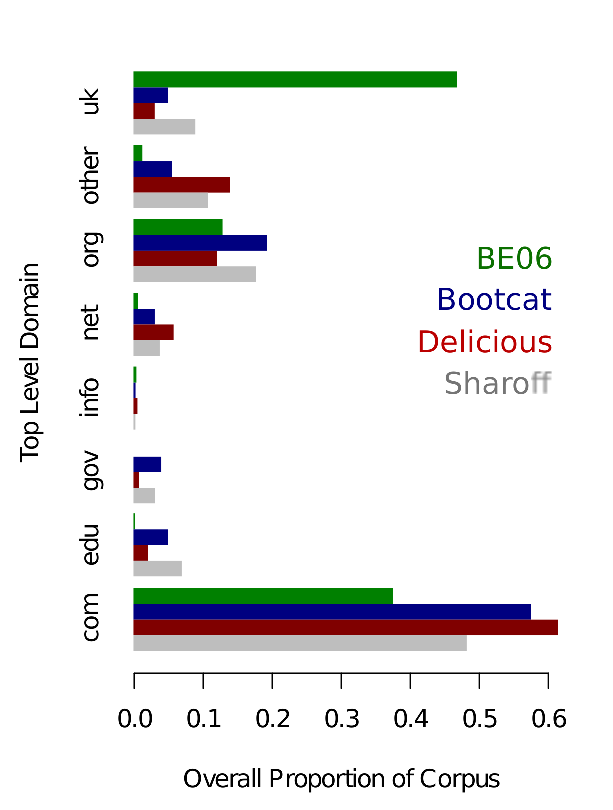
\includegraphics[width=0.6\textwidth]{longitudinal/attrition-all-tlds}
    \caption{Overall distribution of top level domains.}
    \label{fig:longitudinal:attrition:attrition-all-tlds}
\end{figure}





Each of the corpora exhibit similar distributions of each top level domain (TLD), though the large differences in sample size make formal comparison difficult.  The overall distribution of the more popular domains is provided in Figure \ref{fig:longitudinal:attrition:attrition-all-tlds}.  This indicates that \texttt{.com} dominates the selection across corpora, with \texttt{.org} following.  Only BE06 differs from this distribution in its selection of \texttt{.uk} addresses, however, it has been deliberately biased this way so as to represent British English.


Other studies have identified statistically significant differences in the rate of attrition between the major TLDs.  
Though each corpus exhibits a dependence between these TLD groups (chosen to represent the vast majority of each corpus' content) in a $\chi^2$ indepdence test ($\chi^2 > 33.8; p<0.01$ in all cases), generalised linear models reveal that the nature of this dependence varies greatly between corpora, indicating that this estimate is far too simplistic to represent the real causes of attrition.


%a more detailed model does not display any reveal significant differences between those identified in other studies.  For each of the four sample corpora, \texttt{.edu}, \texttt{.info} and \texttt{.org} display similar rates of attrition to \texttt{.com} and \texttt{.uk}.  It seems reasonable to conclude that this effect is as a result of the low frequency of certain more obscure TLDs such as \texttt{.tv}, many of which are revealed to be significant when predicting loss for each corpus using a logistic regression model.




%In accordance with other studies on more general-purpose web content, there are minor observable differences between TLD longevity, with \texttt{.edu}, \texttt{.info} and \texttt{.org} displaying lower rates of attrition overally than \texttt{.com} or \texttt{.uk}.  
%These differences are not statistically significant, however, for any of the corpora used.


% TODO, possibly graphs.  This would be nice to cut if I run out of space since it's only confirmatory and there are few patterns between the corpora














%t URI PATH LENGTH
    %> plot(  density(be.s3$uri_npath)  )
    %> plot(  density(deli.s3$uri_npath)  )
    %> plot(  density(boot.s3$uri_npath)  )
    %> plot(  density(serge.s3$uri_npath)  )
The shape of the empirical distribution for path length of the URI is shown in Figure \ref{fig:longitudinal:attrition:attrition-density}.  Delicious.com users may be expected to bookmark top-level domains with relative frequency, but the difference between the two BootCat samples is more subtle, perhaps an effect of search engine changes.  The preponderance of introductory or `launch' pages in the Delicious data set may also go some way to explaining the longevity of its content --- it seems reasonable to presume that top-level pages remain online for longer (though also perhaps that they change more often).

    %The shape of the empirical distribution for the path length of the URI varies between the Delicious and search-engine-built corpora (figure \ref{fig:res:dist}), with users of Delicious more likely to bookmark top-level domains.  This indicates a preponderance of introductory or `launch' pages compared to the other corpora, which exhibit a more bell-like curve that appears more rational as a cross-sectional sample of website URIs.

\begin{figure}[Ht]
    \centering
    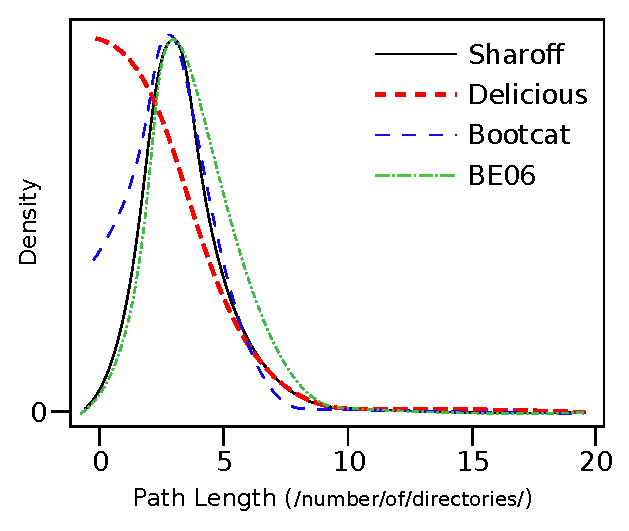
\includegraphics[width=0.8\textwidth]{longitudinal/attrition-density}
    \caption{Differences in the empirical distribution of URI path length.}
    \label{fig:longitudinal:attrition:attrition-density}
\end{figure}


% URI ARGUMENTS (dynamic-ness)
% SUMMARY OF ARGUMENTS
    %> summary(factor(be.s3$uri_nargs))
      %0   1   2   3   4 
    %353  58  47   6   1 
    %> summary(factor(deli.s3$uri_nargs))
	 %0      1      2      3      4      5      6      7      8      9     10 
    %579415  36137   8276   2445   1166    459    205    116     76     45     15 
	%11     12     13     14     15     16     17     19     29     30 
	%11     12     10      3      1      2      1      1      1      1 
    %> summary(factor(serge.s3$uri_nargs))
	%0     1     2     3     4     5     6     7     8     9 
    %68176  8637  2905  1434   458   202    65    12    19     2 
    %> summary(factor(boot.s3$uri_nargs))
	 %0      1      2      3      4      5      6      7      8      9     10 
    %165894   7339   2039    633    294    129     37     29      4     20     13 
	%11     12     15     18     20 
	 %1      3      1      1      1 
%ARGC > 0 COUNTS
    %> summary(factor(be.s3$uri_nargs > 0))
    %FALSE  TRUE 
      %353   112  = 23.68%
    %> summary(factor(deli.s3$uri_nargs > 0))
    %FALSE   TRUE  
    %579415  48983  = 8.45%
    %> summary(factor(serge.s3$uri_nargs > 0))
    %FALSE  TRUE 
    %68176 13734  = 16.70%
    %> summary(factor(boot.s3$uri_nargs > 0))
     %FALSE   TRUE 
    %165894  10544  = 5.95%
Taking the presence of GET-arguments in a URI 
as an indicator of a page being dynamic, a number of effects may be seen across the corpora.  The BE06 corpus had 24\% of all links dynamic, exceeding Sharoff's at 17\% and Delicious \& BootCat at 8\% and 6\% respectively.  This difference is probably due to the selection of published documents, since the compiler was seeking specific materials within sites rather than attempting to retain the location of a resource (as with Delicious) or sampling randomly from URI-space (as with BootCat).  Differences between the two BootCat-based corpora may reflect changing weights within search engine algorithms. %TODO: which may also use this property as an indicator, amongst other things











%--------------------------------------------------------------------------------

\subsection{Discussion}

% these next three bits may be better in the conclusion/future-work section
%In addition, the searching model for WaC samples language through search engine APIs which apply a lens of common usefulness in their modelling of search results. This lens represents a consumption-based sampling strategy, rather than one of production. This may also have implications for the WaC paradigm in terms of the resulting language sample.

%The decentralised architecture of the web has great implications for online content availability --- whereas some sites are large, publishing and holding content for authors, others constitute a single, self-published work.  The distinction between these is weak online, and, crucially, tied to the topic and purpose of the text itself.  

%It seems reasonable, for example, to state that news websites are generally more long-lived than personal or hobby websites, which are backed by individuals.  This attrition of documents online may cause skew in the representativeness of any samples taken from an open-source corpus, as well as producing a drift in any results computed from web-as-corpus studies (especially those with small sample sizes or specialised subject areas).


These preliminary results indicate that the process of corpus compilation, by introducing deliberate bias into the content  (the selection of full documents, filtering of navigation pages, etc.), impacts the observed document attrition rate.  These biases have been evidenced by the URI features alone, raising interesting questions about the effect that collection strategies have upon corpus integrity --- should the tendencies of different groups of web publishers be factored into sampling strategies for open-source or subject-specific corpora?

The ramifications of these biases for the WaC availability sampling strategy remain an open question --- does `searching' for links imply a minimum age, and hence a pre-existing skew towards certain content?

% rephrase? not sure about 'observe' and what you mean here
There are indications that sampling a cross-section of production, rather than consumption, observes the initial steep decline in document availability that is inherent in most survival distributions%( mention exponential vs bathtub shaped curve?, nope-SW)
.  It is possible that these effects are minimised by the WaC approach, and are actually more pronounced in conventional, offline, corpora: search-based sampling may compensate for this effect by weighting reliable and established websites through the algorithms used to rank relevance, though further work is needed to establish the degree to which this occurs.  Another possible effect is the disproportionate availability of archived, out of copyright, documents.


%These results hint at the scale of the bias applied when selecting documents online, relative to their longevity.  These biases seem to be explainable partially in terms of the findings of other web attrition studies, implying that the method of URI selection is key in discounting pages with dynamic or non-document content (such as navigation, help or launch pages).

%In the best case, where all linguistic areas decay at a similar rate, this merely causes us to question the validity of corpora sampled a short time ago.  Where conclusions depend upon the changing nature of presentation or context this change is likely to be more pronounced, as websites taken down are notionally unlikely to be uploaded without some degree of change.


% TODO: not compensating for server-side 404 error messages

% ------------- Vestigial notes -----------
%1) Different methods of building corpora represent different portions of the web in such a way that affects their longevity
%2) BE06-style sampling of \_production\_ rather than consumption online seems to cause high volatility (bathtub-shaped failure curve?)
%3) Long-term, high-resolution study necessary to idenfity patterns of loss over a year (clustered around tax year?)
%4) study limitations
%    * not compensating for server-generated pseudo-404 messages
%    * Not taking into account changing content/topic (or content at all)
%    * not taking into account role of page (navigation, etc)
%    * wildly heterogenous data sources due to availability sample




% -----------------------------------------------------------------------------
\subsubsection{Further Work}
Further sampling and analysis is necessary to confirm the issues highlighted above.  This paper comprises a preliminary look at data sampled in a longitudinal study, which will go on to relate the influences of extrinsic document features (which may be used to inform sampling strategies) to their linguistic content.  

This will involve, primarily, identifying the extent to which document attrition applies bias on linguistic content, rather than technical features, and how this varies through the sampling period.  Issues of particular interest include:

\begin{itemize}
    %\item The extent to which attrition online skews the linguistic content of corpora;%, and if this may be compensated for by careful construction;
    %\item The rate of change of documents online from a semantic, rather than technical, standpoint;
    \item The distribution through time of documents online --- does sampling using search engines apply particular topical bias as they respond to time-critical events?; % regular or lumpy, is this periodic? related to other stuff?
	\item The propensity of document contents to change in meaningful ways (rather than simply updating boilerplate and navigation page code);
    \item Whether similar documents or websites display similar levels of loss;
    \item The characteristics of compilation strategies with regards to their effects on attrition --- is it possible to control biases in web-derived corpora through stratified or two-phase sampling techniques.
\end{itemize}



% ------------- Vestigial notes -----------
% * Analysis of content relative to attrition
% * Analysis of change relative to attrition
% * Analysis of "threshing" and how it affects open source corpora
% * Analysis of the curve of death relative to content/change
% * Topic-distance vs attrition, create a [compensatory] model for topic-space (including nice 3D surface graphs)







\section{LWAC: Longitudinal WaC Sampling}
\label{sec:longitudinal:lwac}


\subsection{Rationale}

Many sampling efforts for linguistic data on the web are heavily focused on producing results comparable to conventional corpora.  These typically take two forms: those based on URI lists (e.g.\ from search results, as in %~\cite{sharoff2006creating}
BE06~\cite{baker2009be06}, BootCat~\cite{baroni2004bootcat}), and those formed through crawling (e.g.\ enTenTen\footnote{\url{http://trac.sketchengine.co.uk/wiki/\\Corpora/enTenTen}}, %~\cite{}, %FIXME
UKWaC~\cite{ferraresi2008introducing}).

Though initial efforts in web-as-corpus (WaC) focused on the former method %, in part due to concerns over the balance of samples returned, 
many projects are now constructing supercorpora, which may themselves be searched with greater precision than the `raw' web, in line with Kilgarriff's vision of linguistic search engines~\cite{kilgarriff2003linguistic}.  This has led to the proliferation of crawlers such as those used in~\cite{schafer8building} and WebCorp\footnote{\url{http://www.webcorp.org.uk/live/
}}~\cite{renouf2003webcorp}.

% diachronic work with webcorp.
% \cite{kehoe2006diachronic}
% \cite{kehoe2009weaving}

This approach, with its base in a continually-growing supercorpus, parallels the strategy of a monitor corpus~\cite{sinclair1982monitor}, and is applicable to linguistic inquiry concerned with diachronic properties~\cite{kehoe2006diachronic}.
%Even for informal searches, tools for date-based lookup are increasingly (e.g. Google).


Repeated sampling by crawling, whilst balanced linguistically, omits subtler technical aspects that govern consumption of data online, most notably the user's impression of its location, as defined by the URI\@.  Low publishing costs online, paired with increasing corporate oversight and reputation management (both personal\cite{ICT4DBibliography1650} 
and professional\cite{Malaga2000repman}), have lead to a situation where this content is being revised frequently, often without users even noticing.

The nature of within-URI change have been studied from a technical perspective by those interested in managing network infrastructure, compiling digital libraries~\cite{tyler2003librarians}, and optimising the maintenance of search engine databases~\cite{koehler2004longitudinal}.  The needs of these parties are quite aside from those of corpus researchers, however, since they focus around a best-effort database of information, rather than a dependable longitudinal sample with known margins for error.

% ---
Current methods for sampling language change online include:

\begin{itemizeTitle}

    \item[Crawlers/Revisiting] Continuously crawl pages, adding new ones as links are updated and revisiting old ones according to heuristics;
    \item[Diachronic corpora] Build two separate corpora using the same sample design at different points in time;
    \item[Monitor corpora] Continuously add new material to a corpus as it is created, agnostic of change;
    \item[Subsampling supercorpora] Build a large corpus and select documents from it according to a bimodal distribution of document age;
    \item[Feed corpora] Crawl pages on publication date (a form of monitor corpus).

\end{itemizeTitle}


Each of these methods is subject to a number of downsides, making them difficult to use for many scientific purposes, or requiring significant resources and forward-planning (thus putting them out of the hands of most researchers).  Some issues, such as irregular revisiting of pages and the lack of detail stored about network-level metadata, complicate the process of analysis.  Most corpus formats are also not annotated by time, meaning that analysis often requires repeated export and comparison --- tools for which must be produced on a case-by-case basis.

% 
% \begin{itemize}
%     \item \textsl{Incremental sampling}---Search engine databases and digital archives are persistent, and may be incrementally updated in a continuous manner whilst still being useful;
%     \item \textsl{Lack of comparability}---A cross-sectional sample of search databses yields documents sampled at various times, with a possible age variation as modelled by the specific type of web page.  This is evidenced well by the relative likelihood of receiving a broken link when searching for current events \textsl{vs.} older scientific articles.
%     \item \textsl{Information-seeking behaviour}---Search engine literature indicates [CITE] that information, when lost from one location, is often available at many others.  This same process is unlikely to be followed, however, if a resource has simply changed, or if a user relies on a small set of web pages as an information resource (such as news sources).
%     \item \textsl{Deliberate `usefulness bias'}---Sources deemed to be pertinent to a search engine's clientelle are sampled more frequently, and thoroughly.  This results in persistence-of-value surrounding high-profile domain names and companies, which dominate the zipfian distribution of web results.
% \end{itemize}
% 


We present here a tool, LWAC, for this form of longitudinal sampling, designed to maximise the comparability of documents downloaded in each sample in terms of their URI rather than content.  To accomplish this, we use a cohort sampling strategy, as illustrated in Figure~\ref{fig:longitudinal:lwac:samples}, to get full coverage over a list of URIs, at the expense of sampling new content.

\begin{figure}[Ht]
    \centering
    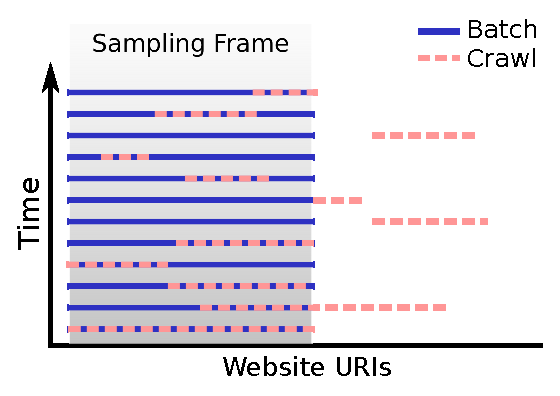
\includegraphics[width=0.6\textwidth]{longitudinal/lwac-samples}
    \caption{URI coverage for batch and crawl}
    \label{fig:longitudinal:lwac:samples}
\end{figure}

This approach allows for reliable re-visits to each member of the sample, and thus the construction of vertically comparable data points, whilst making short-term effects visible by revisiting each link.  Such a sample design should repeat each individual sample as quickly as possible, so as to minimise the time differences between documents within.


This allow a user to investigate how language may change in relation to technical and social events in a way that mimics the experience of many end users, and offers a useful perspective on many epistemic problems of WaC methods, to determine:

\til{Integrate these as an extension of the previous section}

\begin{itemize}
    \item The portions of web pages that typically change as main content regions;
        \vspace{-6pt}
    \item The impact of social feedback and user generated content on page content;
        \vspace{-6pt}
    \item How censorship, redaction and revision affect website contents;
        \vspace{-6pt}
    \item Website resource persistence and its relation to linguistic content (link rot/document attrition);
        \vspace{-6pt}
    \item How institutions' publishing policies affect reporting of current events.
\end{itemize}

LWAC is designed to construct longitudinal samples from URI lists, using only commodity hardware.  It is designed with `full storage' in mind, that is, recording everything about each HTTP session in such a way that it may later be exported and accessed in a parsimonious manner.


LWAC is based around a central corpus store that is indexed both by time and URL\@.  Each sample consists of all datapoints in the corpus, and begins at a specified time: this time is aligned to a sampling interval.

Figure~\ref{fig:longitudinal:lwac:samples} shows the logical structure of the corpus: the blue bars represent each sample.  The primary technical challenge lies in maximising the parallelism of each sample, thus improving the comparability of datapoints therein and allowing for a smaller sampling interval.  Samples that overlap their sampling interval will not be stopped: instead the next sample will be delayed until the next `round' interval.  This eases analysis by ensuring the integrity and temporal alignment of each sample.

Documents are downloaded in a random order, so as to avoid systematic variation in sample times across links.



\subsection{Design \& Implementation}


\begin{figure}[Ht]
    \centering
    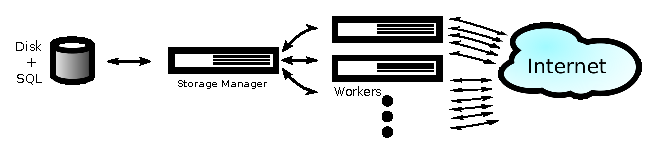
\includegraphics[width=\textwidth]{longitudinal/lwac-arch}
    \caption{System Architecture}
    \label{fig:longitudinal:lwac:arch}
\end{figure}


In order to perform the parallel retrieval stage quickly, LWAC is constructed as a distributed system, with a series of workers performing the page retrieval and passing batches of data to an offline system for further processing.  This architecture, shown in Figure~\ref{fig:longitudinal:lwac:arch} is extensible until the limit of contention for the storage manager's network connection is reached, which in practice is encountered at many tens of worker nodes.  In addition to the use of multiple workers, each worker performs many parallel requests\footnote{The portion of LWAC used for parallel request management is available separately at \url{https://rubygems.org/gems/blat}}.

The storage manager is responsible for all scheduling and data integrity: workers are treated as (relatively) untrusted actors, and allocated batches of links on request.  The scheduling system monitors performance of each worker, and dynamically computes a timeout for work units: exceeding this timeout will see the batch of links re-assigned to another worker.  This system allows for great flexibility in workers, which may vary in batch size and connection throughput.

The storage manager is also responsible for enforcing atomicity of jobs and of the underlying corpus.  This is enforced using a check-out system: workers check out batches of links that remain allocated until they are returned, completed, by the same worker.  When a sample is complete, it is `sealed' on disk to prevent further edits, and the scheduler instructs workers to sleep until the next sample time.


The corpus itself is structured as a root directory, containing a specific structure:

\begin{lstlisting}[language=,caption={Corpus directory structure on-disk},label=lst:longitudinal:lwac:corpusformat]
root/
root/database.db
root/state
root/files/sample\_id/sample
root/files/sample\_id/1/2/3/456
\end{lstlisting}

% The metadata database (if using SQLite3)
% The state of the current sample. This is stored as a serialised ruby object so that a sample may be resumed later if the server is stopped.
% A list of sample ID folders containing:
% A file describing the properties of this sample as a serialised ruby Sample object
% A structure of directories describing link IDs, each of which has up to N files within it (as defined in the server config). This structure uses the first characters of the ID to nest directories in order to avoid filesystem limits on inode size and speed up random access, i.e.: 0/1/1 0/1/2 0/1/3 0/2/1 0/2/2 0/2/3 etc.


Data storage in the system is split between metadata, stored in an SQL database, and website sample data itself, which is stored as raw HTTP response data in a versioned structure on disk.  The storage format is optimised for large samples, and is nested in order to avoid common filesystem limits (as shown in Listing~\ref{lst:longitudinal:lwac:corpusformat}
).  LWAC does not enumerate URIs in memory, meaning there is no hard limit on corpus size --- instead it incrementally loads links as requested by the workers.  This means that memory usage is limited to the maximum batch size within the system.

Workers are able to imitate the behaviour of end users' browsers as much as possible, so as to avoid search engine optimisation and user-agent detection tactics.  They are able to provide cookies and request headers commensurate with a web browser, and follow redirects to similar depths.  This behaviour is passed as part of the work unit itself, and so is configured centrally.

Workers are able to enforce limits on MIME type and file size, ensuring that documents are not downloaded if they are incompatible with further evaluation stages.

After downloads have occurred, data may be retrieved for analysis in a variety of formats using the included export tool.  Export is possible at one of three levels: all data, individual samples (all datapoints at a given time), or individual datapoints (across all times).


Metadata is stored about network-level properties such as timeouts and latencies, as well as URL properties (link length, etc.) and HTTP headers.  The original request parameters and sample design are also presented in the same structure, allowing corpora to be somewhat self-documenting.  Appendix~\ref{sec:appx:fields} shows the object hierarchy of page data.


Exports are performed by filtering data using a series of expressions.  These data are then passed to formatting expressions, which are able to normalise display formats for analysis, before calling a number of pluggable formatting modules.  Current formats supported are:

\begin{itemize}
    \item CSV format with one-row-per-datapoint or per-sample;
    \item A collection of CSV files, split per-sample;
    \item JSON collections, for import into tools such as MongoDB;
    \item Arbitrary text output using the ERB template format.  Supports server, sample and datapoint level exporting;
    \item XML, transformed from the original input parameters using XSLT.
\end{itemize}



\subsubsection{Resource Usage}

LWAC is designed to handle corpora of theoretically infinite size, and uses a pipelined design to avoid enumerating its corpus members.  In practice the limit on corpus size is imposed by the SQL server used.

Memory usage is $O(1)$ for both the storage server (which backs all of its corpus data with the disk) and the client (which only ever loads as many datapoints as number of parallel connections).  Ultimate limits are defined by the batch size chosen for workers:

\begin{itemize}
    \item Server: $(\textit{clients} \times \textit{batch\_size} \times \textit{link\_size}) + (\textit{batch\_size} \times \textit{max\_resource\_size})$
    \item Client: $\textit{in\_progress} \times \textit{max\_resource\_size}$ (using disk cache)
\end{itemize}

Workers use static quantities of disk, equal to the maximum download size of each page multiplied by the batch size.  Disk usage for the storage controller is $O(N)$,  though the storage format is well suited to deduplication using symlinks to point to previous data.


\subsection{Performance}
Ultimate performance is dependent on a number of factors:

\begin{itemize}
    \item The number of worker machines used;
    \item The number of connections per worker;
    \item Worker network speeds;
    \item Latency of DNS and web servers.
\end{itemize}

The last of these implies gradual degradation of performance as links rot.  Performance figures stated here are therefore for the `best case' scenario where links are all available from fast servers.


\subsubsection{Artificial}


\begin{figure}[Ht]
    \centering
    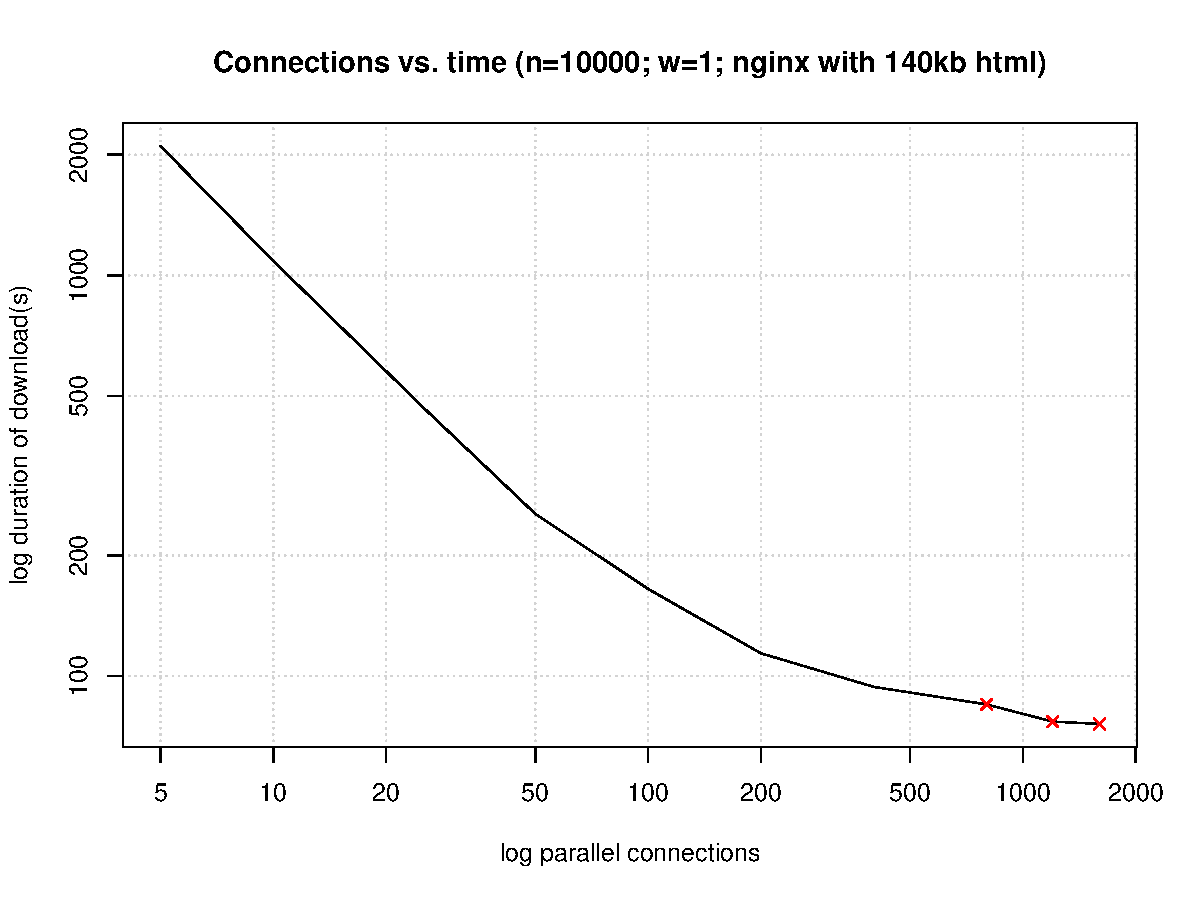
\includegraphics[width=\textwidth]{longitudinal/lwac-parallelrate}
    \caption{Download speeds for one worker for various levels of parallelism}
    \label{fig:longitudinal:lwac:parallelrate}
\end{figure}

Figure~\ref{fig:longitudinal:lwac:parallelrate} shows the download rate for 140KiB HTML files served over 100Mbit ethernet using the Nginx web server.  This server configuration was designed to offer high-performance yet still be representative of common web deployments\footnote{Nginx is known for its ability to serve many users at once, and ``[a]ccording to Netcraft, nginx served or proxied 21.64\% busiest sites in May 2015.''---\url{http://nginx.org/en/}}.

The performance of parallel downloads is largely constrained by the platform, in this case the Linux 2.6 kernel.  Downloads are reliable until roughly 700 parallel connections are used, beyond which requests are dropped locally as half-open sockets are closed.  Until this point performance is roughly log-linear, with 100,000 requests taking just 100 seconds with 500 parallel connections.

For subsequent tests, 400 connections per worker machine were used.


\begin{figure}[Ht]
    \centering
    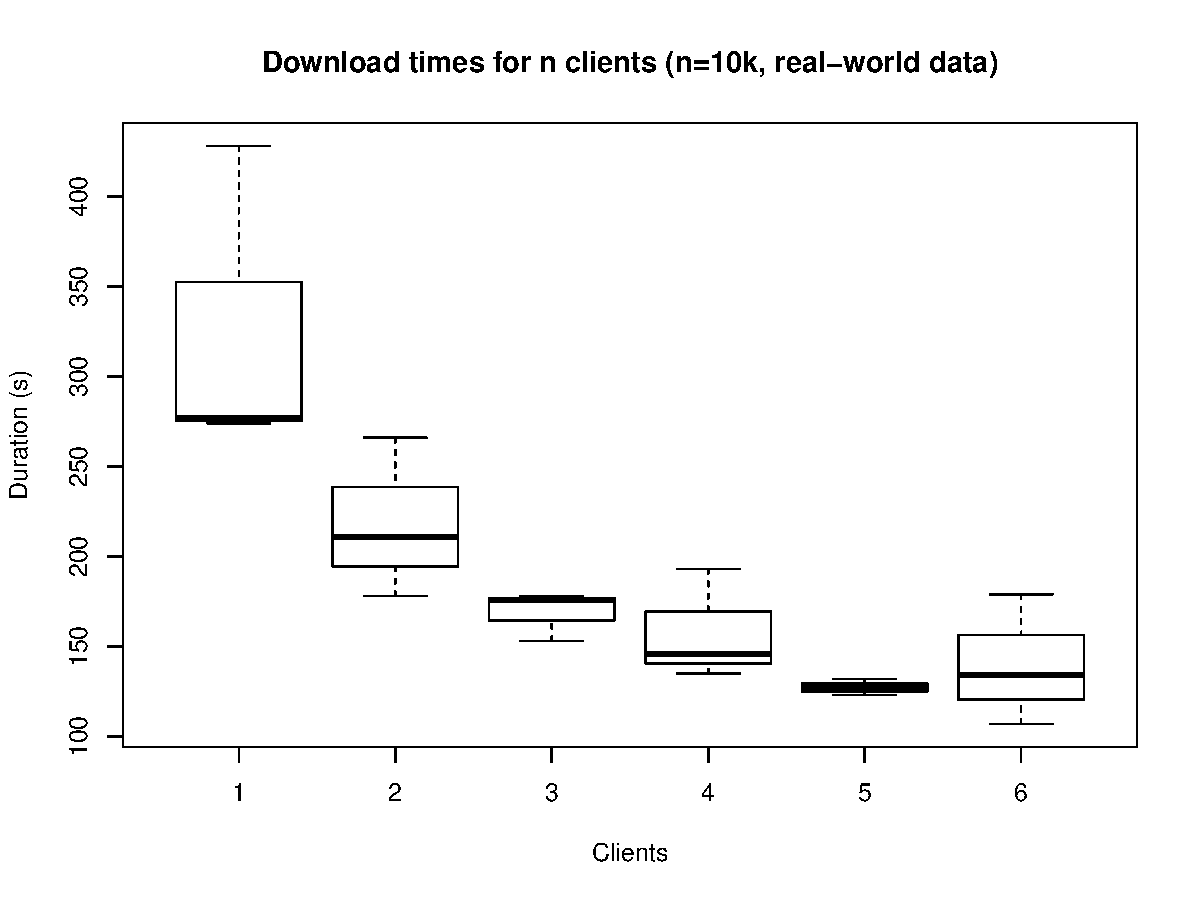
\includegraphics[width=\textwidth]{longitudinal/lwac-clientrate}
    \caption{Download speeds for 10,000 real-world HTML documents.}
    \label{fig:longitudinal:lwac:numclients}
\end{figure}


Selecting the number of worker machines required for a deployment is a tradeoff between many factors, particularly cost and download rate\footnote{Reliability and physical location are also likely to influence results, especially where geography affects the contents of pages}.  As the server is responsible for all co-ordination, the speed improvements seen when adding worker machines is nonlinear, eventually plateauing where the overhead of the batch request equals the difference in time between requests made by $n$ and $n + 1$ workers.

Figure~\ref{fig:longitudinal:lwac:numclients} shows the overall download times for the same dataset when using differing numbers of workers.  Workers were all connected to the storage manager via 100Mbit ethernet (minimising contention), and were making requests via the same link to a local test machine.  As expected, the improvements soon plateau, though there is a large amount of variance --- larger batch sizes and a larger test corpus are expected to show further improvement with $n > 6$\footnote{Procuring machines for this experiment was tricky, as they could not be virtualised}.  This plateau may be expected to occur earlier if workers are connected via relatively low-bandwidth links (for example, if they are connected over long distances via the internet or a VPN).





\subsubsection{Real-world}

In order to test retrieval performance in a real-world scenario, a test deployment was constructed consisting of three clients, each making 400 parallel connections.  Each was running Linux 2.6 connected to the storage manager using a 100Mbit ethernet link, and to the internet using Lancaster University's tier-1 fibre connection.  This setup was designed to be within reach of many academic users, who are likely to have bandwidth allocations exceeding the sites that they visit, yet have limited access to hardware.


The 228,000 URLs used were sourced using BootCaT, making 4600 requests to the Bing search engine and retrieving 50 links per request.  This resulted in a corpus size of 14.9GiB, which, after boilerplate removal, yielded 588 million words.


\begin{figure}[Ht]
    \centering
    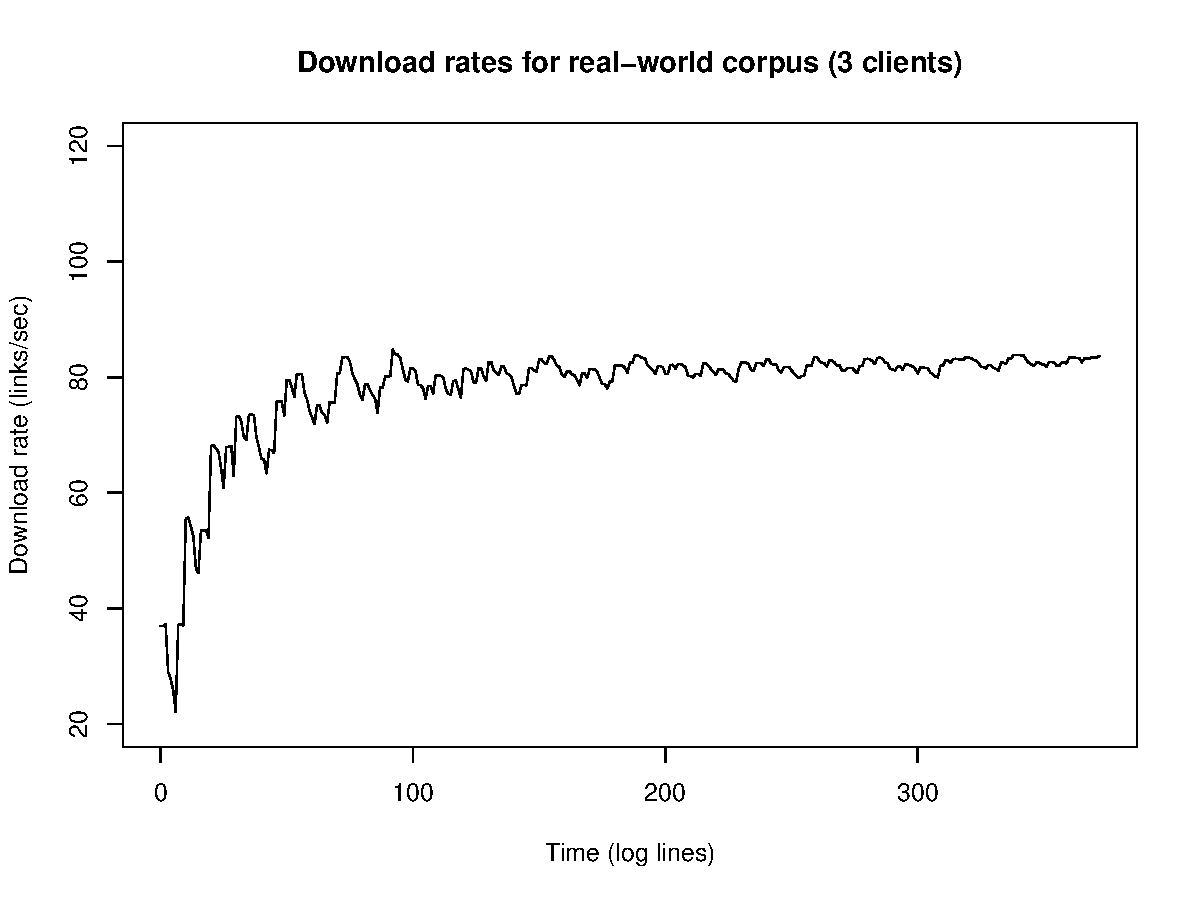
\includegraphics[width=\textwidth]{longitudinal/lwac-realrate400}
    \caption{Download rate over time for real-world BootCaT derived dataset.}
    \label{fig:longitudinal:lwac:realrate400}
\end{figure}

The throughput over time is shown in Figure~\ref{fig:longitudinal:lwac:realrate400}.  This data was summarised by examining the logs of the storage manager, and thus represents rate calculated after each worker has checked in its batch --- hence the pattern of jagged increases followed by gradual decay.  Larger spikes are seen towards the left hand side due to synchronisation of the check-ins by clients: eventually variations in batch retrieval times cause these to disperse and smooth out.  This deployment can be seen to plateau at roughly 80 links per second (roughly 288,000 per hour), meaning the full 228,000 page corpus was retrieved in roughly 45 minutes.

Using this deployment would mean that retrieval of a corpus the size of the BNC is possible in around eight minutes; a ukWaC\cite{ferraresi2008introducing} copy would take 2.5 hours (or 17 if using the pre-filtered url list), and DECOW2012\cite{schafer2012building} would take 24 hours. \td{cite these?}





\subsubsection{Etiquette}
Ordinarily, crawlers are expected to adhere to well-acknowledged guidelines regarding page retrieval, revisit times, and link traversal.  LWAC ignores these by design, due to a number of factors that differentiate it from standard crawlers.

Firstly, the integrity of the returned samples is impossible to validate if they are not reliably retrieved.  Any missing data would have to be imputed, reducing its scientific value and complicating the process of analysing results.

Secondly, though this is largely under the control of the user, it is expected that links will not be visited so regularly as to significantly increase load on a given server.  Most effects requiring longitudinal analysis take place over a relatively long period of time that does not warrant short sample periods.

Finally, LWAC's link selection is unlikely to include many pages hosted on the same server.  This is not guaranteed, however, for web-wide longitudinal analyses each `hit' by LWAC is not going to result in immediate successive hits to the same server, as it would with a crawler that navigates pages.  Where this is violated, it is of course up to the user to mitigate any load to the web server.  LWAC's randomisation of the order of link traversal also helps mitigate this, as it reduces the chances of a set of links co-occuring systematically in each sample.

Though it is possible to perform DDOS-style attacks using LWAC, the use-case for which it was designed is unlikely to violate the principles adhered to by existing crawlers.






% Currently, workers do not interpret JavasScript or construct a DOM






\section{Summary}
\label{sec:longitudinal:summary}

There are a number of methodological challenges that continue to prevent application of the methods described here to larger populations.  These are either due to the problems inherent in sampling varied data in the first place (digitising photographs or transcribing audio), or the processing required to transform data into a usable form (models of attention).

It is hoped that further work will be able to develop these methods in order to mitigate these issues, at least for certain applications.  However, the utility of these methods to the thesis is retained under less ambitious conditions of restricting a combinatino of the domain (for example, only sampling web histories or work-day language use) and the population (i.e. only people very similar to myself).

The practical issues encountered during sampling are largely minor, and modern portable technology proved decisive in making capture of hitherto-unseen (or at least widely ignored) sources of text possible in-the-field.  The census design lends an empirical justification to inclusion of these genres in larger general-purpose corpora, however, we are unable to formally generalise with confidence to demographics other than that of the subject covered.

Of particular note (and perhaps greatest generalisability) is the number of words used throughout the sampling period.  Almost a million words were input and output by a single individual over a two week period.  Since it is reasonable to deduce that this sampling is at best representative only of a normal working week for a single individual, it is rational to suppose that a corpus purporting to cover the whole population of a country demands a sample size far greater than many existing corpora.


This would seem to form an argument that it is simply not cost-effective to build a conventional general-purpose corpus large enough to represent large populations, suggesting that the focus should lie in those built for more specialist purposes, or those sampled non-probabilistically.  Here, the extreme size of web corpora may be well justified, so long as they can be shown to have been sampled rigorously.


This suggestion is reinforced by the obvious variability in the proportions of texts taken from each source, which will vary greatly by lifestyle.  Indeed, it seems that the measure of one's lifestyle by text source is a particularly direct way of characterising inter-person variability, and further work may be focused on this problem as a way of simplifying the methods described here.


Of interest to this thesis is the high level of detail that may be captured using this method.  The census design affords full coverage of a given area about which we may wish to generalise, and the detail it is possible to capture this way makes the data ideal as a `seed' for constructing larger corpora with comparable properties.  Application of these methods, as well as those using auxiliary data mentioned above, will hopefully render this sampling method a complementary one, to be added to the collection of existing corpus designs.

\til{Link back to main themes of thesis}






\chapter{Proportionality: A Case Study}
\label{sec:personal}
\section{Introduction}
The degree to which a general purpose corpus represents ``real'' language use is often debated at length, and is the key issue affecting design of corpora.  A wide variety of methods have been used to estimate language proportions and usage for a whole population, however, these are mediated by (and often centre around), expert opinion.

Reasons for this approach are both theoretical and practical---sampling individuals in the act of using language is very difficult (something other social sciences also struggle with), and the persistent nature of texts means that they conceptually stand alone, especially where the corpus designers intend to include older works.

Nonetheless, there is a missing empirical link between the expert-guided designs of language proportions and the ground truth of an individual's language use.  This is lamented by many who wish to study language acquisition (or more detailed explanatory theories regarding language use over time \td{cite Hoey, quote too}.

This chapter describes a case study whereby a census of text types was attempted for a single individual.  This sample design yields very little inferential power regarding the whole population, but serves to illustrate the disparity between the proportions a general purpose corpus may have, and the language used by an example individual.  The extent to which this example individual may be a useful guide for corpus building is not addressed directly, but this is an area that could be expanded using demographic auxiliary data.















% ============================================================================
\section{Sample Design}
As we have seen in chapters~\ref{}\td{ref}, conventional corpus building efforts centre around linguistic variables, and rely largely on expert opinion to balance their socioeconomic variables.  This approach was initially selected in order to avoid certain practical problems (many of them caused by technological limitations), though it has also caused others, most notably the difficulty in retrieving metadata about texts post-hoc.

Often, the only way to ensure demographic balance is to rely on sources of auxiliary data such as bestseller lists and library loan records that map textual variables to socioeconomic ones.  This process of using `proxy' variables is particularly opaque, and often limits the metadata available.

The intent of this chapter is to sample in an ad-hoc manner, that is, to record details of a text or single use of language in context, as it is used.  This approach is far closer to that used in special purpose corpora, especially where the restricted domain allows use of automated recording tools or sampling from an existing rich database (such as from an online forum).

The case study itself takes the form of a census of language use, for a given period, for a given person.  This offers empirical validity for linguistic proportions, but is a single data point from the population of language users and cannot be formally generalised.

Of particular interest are variables that are particularly challenging to sample:

\begin{itemize}
    \item The age of a text when ``used''
    \item Other temporal information, such as the times and days when texts are read, and inter-day variance etc.
    \item The social context of text use
    \item Attention paid to a text, and which portions were read
    \item Proportions of text types used, especially representation of types that may be missing from other corpora such as greetings, billboards, product labels.
\end{itemize}

The ad-hoc sampling approach, applied to \textsl{all} texts used, also allows inspection of the proportions of language types used---something that is estimated for general purpose corpora.  Though the scope of this case study is necessarily limited, a ``language use census'' for many people would be a robust empirical method for validating claims of representativeness in GP corpora.


A further advantage of this method is that the population may be rigorously defined, as data on the participants is available to whatever standard deemed necessary.  This is notably at odds with the use of existing lists or repositories, which have been constructed with differing purposes and levels of documentation.






\subsection{Difficulties and Disadvantages}
Sampling language use ad-hoc involves changes in sampling strategy that are practically challenging.  Taking this study as an example, one would have to take data from enough people to cover the population required, and each would have to undertake a fairly in-depth procedure.

Difficulties encountered when trying to sample large populations are well documented in the social sciences, and many techniques exist to mitigate common biases (\td{such as}), however, these are largely beyond the scope of this chapter.  It is notable that one solution in sociology has been to share data (in a style similar to corpus linguistics) in order to minimise the costs involved in implementing a high quality survey.

The increased ``person-focused''ness of a primarily social design also raises a number of ethical issues, as it is increasingly possible to derive information not just about a general group's language preferences, but about an individual's (or a comparison between groups).  This is merely the inverse of its value, but it is nonetheless worth considering as many study designs in linguistics need not work with such sensitive data.  This issue is addressed after the discussion of methods and findings\td{Ensure that it is.}.

Further, sampling text as it is used raises methodological challenges---how can we be sure that the language observed is still naturally occurring and valid?  All sampling is going to compromise on this, and the extent to which one values detail over interruption will vary by study design.  The aims of this study are, in part, to identify major challenges in this area, for example, which text types are most difficult to sample or require most time to record.














% ============================================================================
\section{Technology}
As mentioned, a number of the limitations to this kind of sampling may be addressed through the application of new and emerging technologies.  This takes two main forms:

\begin{itemize}
    \item Many more documents are now poduced and consumed in digital form.  This means they are accessible for automatic copying and processing by sampling software, often without any intervention necessary by the user.
    \item The abundance and ubiquity of portable technology such as smartphones lowers the difficulty of many existing sampling methods such as audio recording or photography.
\end{itemize}


The former of these is well represented by the WaC movement in corpus linguistics, and many corpora include sections which have been sampled by distributing portable technology\til{So, er, this is where the lit review seems out of place 'cause it's in chapter 2}.  Of particular interest, however, is the value that we may extract by exploiting both to form a coherent narrative.

One community that has been using these techniques extensively is that associated with life-logging.  Life-loggers do stuff---see lit review.










\subsection{Life Logging}
Just as the availability of portable recording technology made acquisition of spoken corpora relatively easy to control, so have the limitations on digitisation and format conversion limited the selection of written text to those already-indexed properties.  As modern computing devices have miniturised and become ubiquitous, they have developed a number of capacities that may be used to afford the same ``instantly recordable'' status to non-spoken language use.


A number of these technologies are as a direct result of the life-logging community's interest in multimedia records.  Life logging is an activity that emerged slowly out of the principles of webcam shows and reality TV.  It involves recording (and usually broadcasting) continuous information about one's life as it occurs.

Though most popular efforts started as a means for providing entertainment, and thus focused on multimedia broadcasting on the web, the techniques required soon diversified and gained the interest of the information retrieval and processing communities.  Many projects have been started with an aim to catalogue and operationalise the huge stream of data each person creates, largely with a focus on aiding that person in their daily life, or aiding large organisations (such as defence forces) in management of resources and people.

\til{citations and a proper lit review, but they are maybe better off elsewhere}

Because of the continuous nature of life-logging, many efforts have been made to use methods that are easy to maintain, self-contained, and covert.  % CITE
Due to this, as well as the original intent of the life-logging process, much of the effort surrounding life-logging focuses on multi-media sources, and how they may be best combined to form a coherent idea of context.  

Typical sources of data considered include:

\begin{itemizeTitle}
    \item[Video recording] Many life-loggers wear systems that are able to continuously record video in the direction they look, and upload this using mobile networking systems.
    \item[Audio recording] Due to its lower obtrusivity, many efforts surround the analysis of audio logs, and include systems to detect voices and identify events such as making appointments.
    \item[Document storage] With the increase in use of digital-origin documents, some of the more holistic life-logging systems record documents as they are read, with a focus being to integrate this data into the larger picture.  Others scan in their post for later retrieval.
\end{itemizeTitle}

Many of the requirements of a life-logging platform (covert operation, comprehensive data management, context identification) overlap notably with the methods used in covert sociological research and, of particular note for our purposes, those constructing spoken language corpora.

Notably, one of the methods used to create the spoken portion of the BNC was covert recording, where a number of people were provided with tape recorders...
\til{ Quote from BNC documentation }

As illustrated by the BNC's demographic balancing of that portion of their corpus, this ability to directly record data from the field satisfies the disadvantages of text-index-oriented methods of document selection, allowing us access to all of the contextual data at the time of text consumption/production 
\til{perhaps because the time of production and consumption don't differ much for spoken stuff...}

The cost of this is, as felt by all sociological studies, a need to find a sufficiently large and heterogenous sample of people who may record data about their language use (and for long enough for it to be useful to researchers).  This is arguably more difficult in practice than text-index-based methods, and should only be considered at a large scale where the difference is likely to be crucial to a study, nonetheless, large samples exist in sociology as testament to the value such designs may yield [and the illustration that no alternative method exists for many sociological issues].

The benefit of having a clearly-defined population about which to generalise linguistic findings is applicable to any size sample, however, making techniques of logging particularly applicable to special-purpose corpora, especially where those corpora are best demarcked along social lines.  Indeed, at one extreme of this scale exists the concept of a personal corpus; something that may yield insights or models about a single person's current language usage.  Such a resource may one day be particularly valuable in defining how one uses text-based interactive systems (such as the web), reads content (such as news articles) or even how one would learn.

Such designs exhibit a tradeoff: a decrease in socioeconomic breadth in exchange for an increase in linguistic breadth.  It is my intent to illustrate the value in this approach, and to investigate methods by which it is possible to construct corpora without undue difficulty through the use of life-logging methods.
% This needs mega elucidation, methinks



\til{ Intro to life logging, a good lit review needs to be done.  Perhaps it belongs in the lit review section rather than here though.}

















% ============================================================================
\section{Approach \& RQs}
The case study described here is an attempt to assess the extent to which techniques from life-logging may assist corpus builders in creasing a demographically-oriented corpus.

It follows an iterative design surrounding these aims, with each iteration refining a number of key design areas:

\begin{itemize}
    \item The variables that may practically be recorded about a text (and that must be before they are lost);
    \item Methods that may be used to sample text unobtrusively, especially how new technologies may be used to assist;
    \item Methods and tools for operationalising logs after sampling is complete, and how these may assist the process of data gathering itself.
\end{itemize}
\til{I'm sure I'm missing stuff here.  Check notes and presentations}

Ultimately, the differences in sample design contribute to a larger picture that could yield much future work.  The direct research questions addressed here are:

\begin{itemize}
    \item What methods may be used for gathering data in a short-term language census?
    \item How may the collected data be operationalised?
    \item What proportions of language are used by the subject; do these support common claims from general purpose corpora?
    \item How may these methods be used in future to aid those building corpora?
\end{itemize}







\subsection{Sampling Policy}
\label{sec:personal:samplingpolicy}
\td{from notes}
The aim of a personal corpus is to emulate, as closely as possible, a census of observed language.

Use of language, in this context, is defined as any conveyance of information, spoken or written, in any quantity. There are no bounds to the context in which it is used, nor the language itself, as the purpose of the study is to evaluate these very things.

Each of these transactions is recorded as a single line in the data set, and will be annotated with the variables recorded.  One of the major issues encountered in preliminary tests was annotation for attention and proportions read.  These will be recorded along with textual properties to ease operationalisation.

Attempts were also made to record sufficient data to retrieve the full text of each transaction.  This worked better for some data sources, and much of the case study thus concerns itself with (sometimes estimated) word counts.  Word counts were chosen as a measure of size due to their use in other corpora, and their applicability to many different media.


A number of practical challenges were identified before sampling, and these were backed up by experience:
\begin{itemizeTitle}
    \item[Review and Production] Both should be recorded as fully as possible. Where a text is re-read, or developed and continually re-read, this should be noted as an ongoing process (and accordingly oversampled).
    \item[Short Utterances] Very short interactions, such as passing greetings, should not be under-recorded. Their inclusion is likely to be one major difference from conventional corpora.
    \item[Oft-reread Texts] such as labels, signs and the like. It’s debatable whether or not one actually reads or merely remembers/recognises these. Perhaps psychological literature (Gestalt, etc.) can shed some light on this?
% See Wang, Zhe, and Gemmell, Jim, Clean Living: Eliminating Near-Duplicates in Lifetime Personal Storage, Microsoft Research Technical Report MSR-TR-2006-30, March 2006.
\end{itemizeTitle}










% ============================================================================
\section{Method}
As mentioned in~\ref{sec:personal:samplingpolicy}, the primary objective of the sampling is to record all ``linguistic events'' for a given period, for a given subject.

The subject chosen was myself---this was done for a number of reasons:

Firstly, legal and ethical issues surrounding recording and review of the data were mitigated by having the analysis performed by a member of the original conversations, etc.

Secondly, iterative review of methods involved was possible with internal, `white box' examination of how data were collected, and what edge cases and procedural difficulties arose.

Thirdly, the demographic status and other person-related variables are well known and need no formal elicitation, minimising time spent on construction of questionnaires et al.


\subsection{Data Sources}
Before the first iteration of the sampling/review process, all of the possible language data sources used in everyday life of the subject were informally identified.  It soon became clear that these data sources exhibited properties that would make sampling easier, or less intrusive.  They were classified by the methods required to capture their text:

\begin{itemizeTitle}
    \item[Persistent] Resources that exist in a format that is easily retrieved and immutable.  This covers many physical items such as books, and some broadcast media as well as notes made in a notebook.  Only identifying information must be stored during sampling itself, in some cases merely an ISBN or similar index code.
    \item[Ephemeral] Language data that cannot be accessed after-the-fact in any way, or may differ by time or context.  This most obviously contains speech, but also many websites, things such as billboards that cannot be readily re-accessed, or todo lists that get destroyed.
    \item[Digital Origin] Documents that are read, or written, on electronic devices.  These may fall into either of the above categories, yet they may usually be copied with no overhead so it is often simpler to store them at the time of use.  Many document types are now digital, as well as the obvious sources such as email or online chat.
\end{itemizeTitle}

This classification was useful in order to minimise the intrusiveness of a collection method, whilst maximising the detail recorded for a given source (ideally to the point of storing verbatim text).  In practice, methods were easy to develop for automated recording of digital documents, and many techniques exist for sampling non-digital persistent and ephemeral sources with scientific levels of accuracy already.

The sources identified in the initial case study were as follows:

\td{Merge these two lists with a separator or something?}
\begin{itemize}
    \item Speech
    \item Printed documents (i.e.\ letters, brochures)
    \item Digital documents (same, but unprinted)
    \item Terminal logs
    \item IRC logs
    \item Email
    \item Websites
    \item Irregularly formatted printed material (posters, labels, advertising on vehicles, billboards, etc.)
\end{itemize}

The inadequacies of introspective methods to identify these soon became apparent during preliminary tests, as the process of recording increased awareness of language use, raising a series of edge cases.  These were collected and resulted in a final selection of sources displayed below.  As well as expending the set of sources to be gathered, methods of collection were chosen with flexibility in mind in order to cope with unenvisaged sources of data\footnote{This flexibility has the unwelcome effect of slowing down analysis later on, and may be undesirable in some cases}.

\begin{itemize}
    \item Speech
    \item Printed documents (i.e.\ letters, brochures)
    \item Digital documents (same, but unprinted)
    \item Terminal logs
    \item IRC logs
    \item Email
    \item Websites
    \item Irregularly formatted printed material (posters, labels, advertising on vehicles, billboards, etc.)
    %---
    \item Written (but non-OCRable) material
    \item Key strokes
    \item SMS records
    \item Phone conversations (separated from speech as they yield differing metadata)
    \item Music tracks
    \item Files accessed
\end{itemize}

This list is necessarily furnished according to the life of the subject in question---from this study I am unable to assert that it is generalisable to others, though the process of doing so would involve relatively little intrusive sampling\td{link to further work}.

Each of these sources is ``covered'' by one or more sampling tools.  These tools progressed most during the iterative process, and each was subject to a number of procedural subtleties that were refined throughout the study.












\subsection{Recording Methods}
Recording methods were chosen for a variety of reasons.  First and foremost they must, in sum, cover the sources mentioned above.  Secondly, they were selected in order to be unobtrusive both for the experimenter and those around him.  Thirdly, they were selected to be flexible enough to cover unforseen contexts and data sources.

The methods used can be separated further into two groups: many methods are capable of recording multiple sources, and serve to form a narrative that describes the metadata of a linguistic event, pointing at another source for the data itself.  These methods were chosen to allow for post-hoc ``memory jogging'' and narrative creation, something that was added to the experimental procedure after the first iteration indicated how difficult to operationalise much of the data would be.

The second set of methods are focused on a single data source, typically requiring little to no manual intervention to record it.  Their records are either indexed by time, or by the more flexible methods mentioned above.


\subsubsection{Indexing and Overview}
\paragraph{Journals and Note-taking}

\begin{figure}[p]
\centering
\includegraphics[width=0.8\textwidth]{notebook}
\caption{The `on-line' notebook}
\label{fig:personal:online_notebook}
\end{figure}

Two journals were maintained throughout the sample.  The former of these was an A6 notebook maintained `on-line' as events occurred (pictured in figure~\ref{fig:personal:online_notebook}).  This was used to store durations of conversations, titles of persistent sources, etc.

The second was an off-line journal, maintained at the end of each day in a narrative style.  This blog-like record was intended to reflect in depth on the proportions of text used in each source, and how attentively each linguistic event was engaged in.  The writing of the journal itself was not logged by any other methods.  It was also possible to attach daily records to this journal, and the process of writing it inserted an opportunity to reflect on the mnemonic codes used during the day.  This process is described in context in section~\ref{sec:personal:recording}.

The on-line notebook proved to be the primary indexing method for all other sources of data, and its maintenance was the primary overhead of the study.  Each entry in the notebook was eventually reduced to a compressed form that roughly followed one-line-per-event, storing the time each event occurred, any identifying information deemed necessary for later memory of it, and a duration or other index of word counts.

\til{Insert a picture of one of the scanned days, pointing out the format}

Problems of simultaneous events and split attention were solved in the notes by having a start/stop event for ongoing events, and by using the off-line journal to reflect upon each event.


\paragraph{Audio Recording}
Following work on machine listening, the original intent of audio recording was to capture the occurrence and duration of conversations, as well as any smaller interactions that would otherwise be difficult to capture (such as greetings, thanks when opening doors, etc.)


\begin{figure}[p]
\centering
\includegraphics[width=0.8\textwidth]{dictaphone}
\caption{The audio recorder used}
\label{fig:personal:audiorecorder}
\end{figure}



Capturing was performed with an Olympus 713PC\td{check this, is it PC713?} dictaphone, recording to a suitably sized external card that yielded many days' continuous recording.  Provision was made to download recordings each night and store them with the off-line journal, however, in practice they remained on the recorder until the end of the study.


\begin{figure}[p]
\centering
\includegraphics[width=0.8\textwidth]{clicker}
\caption{The second audio index marker}
\label{fig:personal:clicker}
\end{figure}


Aligning the recorder's output to the events mentioned in the notebook was a tricky process---Though the recorder itself supports index marks, there is a limit of 99, which was deemed riskily low.  Two devices were built to insert absolute silence onto the recording (something that is rare in real life and easy to programmatically detect), the later of which is pictured in figure~\ref{fig:personal:clicker}.  These clickers were to be pressed at the beginning of each conversation, so that voice activity detection could be performed to estimate the word count of each conversation (or, in an ideal world, extract verbatim text).

In practice, the process of tapping the button proved intrusive and, from the perspective of one talking to the subject, suspicious.

The mechanism used for the final iteration of the study was far simpler---the recorder's start time was written in the on-line notebook, and entries therein were keyed by computing the offset between the two times.  Though this incurs a minor overhead in coding the data, it also allows for spontaneous conversations without much overhead, something that is particularly important to the study of text type proportions.



\paragraph{Photographs}
The primary method of capturing ephemeral, irregularly formatted, non-digital texts was photography using a cameraphone.  This method was chosen largely because the ubiquity of smartphones in British society has led to a situation where photographing fairly mundane items is widely unquestioned.

The smartphone used, a Motorola Milestone, also stores time and location data in its photographs using EXIF tags (as well as storing photographs sorted by day).  This metadata meant that there was often no need to file an entry in the on-line notebook, and the cameraphone could simply be used in a very unobtrusive ad-hoc manner.

In earlier iterations of the study, it became apparent that the loud shutter noise made by the Android operating system when taking photographs was problematic.  Though photography of signs, packets and such remained unchallenged, the attention of people nearby was drawn to the weirdo with the cameraphone all too readily.  This was solved partially by (with great difficulty) disabling the noise, though it was still apparent from posture when a photograph was being taken.

There are notably a number of products available that continually take photographs for the purposes of life logging.  These were considered for the study, but their aims are generally to capture each event, rather than specific aspects of selected scenarios.  The ability to consciously specify that the subject was more attentive in some situations (and take pictures accordingly) was judged to outweigh the value of having a continuous record (something much more capably performed by the journals).




\subsubsection{Targeted Methods}
\paragraph{Phone Calls \& SMS Messages}
Both of these are automatically logged by the Android operating system used by the subject, and each was also indexed in the on-line notebook.  The data was extracted using a free application that exported to XML.


\paragraph{IRC}
IRC was logged by construction of a bot.  This bot accompanies the subject into chatrooms and logs all messages observed, applying a rough human interest model to ignore data seen when the user is set to away.


\paragraph{Web}
The SQUID webproxy was configured to log all traffic, and a number of logins were provided---one for each of the subject's internet-enabled devices.

The logs from SQUID store all requests, including advertising/tracking calls, downloading of things never read by the user (i.e. CSS and Javascript) and AJAX calls to partially reload pages.  As such, a large amount of processing was necessary to extract URLs from these logs, and to parse the resultant data into a usable format.

\paragraph{Keylogging/Terminal recording}
Terminals and keyboard input were logged using a custom application that wrapped a terminal, recording the time each character was sent or received to the shell.

Each terminal created started recording to a new log file, storing the time at which it was started and a series of offsets from this time.

\paragraph{Last.fm}
In earlier iterations it was apparent that lyrics in music were being missed as a source of text---all devices capable of playing music were configured to `scrobble' to the last.fm music service during the sampling period.

Though last.fm do not make their data freely available for access, third party tools exist to scrape their website and download detailed logs of tracks listened to.

\paragraph{Files}
Files were identified in a number of ways.

Some, particularly those on which the subject worked and contributed data, were written down in the journals.  This is a precise method of separating what has been read, but might require a large overhead.

Since the subject works entirely on projects and files that reside in a RCS repository, the logs from each commit were used to generate a diff, and this was accessed after the sampling period to identify contributions made.

Another policy that may be used is identification of files by unix mtime (modification) or ctime (creation), however, this is fraught with inaccuracy, as files are liable to be modified on disk many times whilst being edited, and sampling the differences is likely to happen at haphazard times.  Further, this technique would capture many log files and others that have been edited by processes where the subject was not involved linguistically.  By contrast, commits to an RCS are scheduled around logical additions, and are manually pushed so that only deliberately edited files are stored.

Files uploaded whilst on other systems may be uploaded directly to the off-line journal (which, ironically, is online), or stored on a flash drive that was carried specifically for the purpose.  In practice this did not occur during the recording period, though experience suggests these contingencies would be necessary if a longer sample were taken.

\paragraph{Email}
Emails are, again, stored automatically with sufficient metadata as to make them self-documenting.  However, rather than presume all were read in a given day, each was tagged after being read with a label corresponding to the day.

At the end of the sampling period, these tags were collected and downloaded in mbox format, whence they were processed by the operationalisation script.









\subsection{Recording Procedure}
\label{sec:personal:recording}
The recording process was, as mentioned, structured around each day.

Upon waking, and before any language was used, the recorder was turned on and a note of the time at which this occurred was made in the on-line notebook.  Recording was then continued until the end of the day without interruption.

The on-line notebook, cameraphone, and flash drive, were carried at all times.  Since each of these could be backed up (the cameraphone even did this backup automatically), the most data at risk was a single day.

Notebook entries were made as soon as was possible without interrupting the linguistic event being recorded.

At the end of the day (immediately prior to sleep), a journal entry was written in the off-line journal, and SQUID logs were uploaded for the day.  This journal entry forms a narrative, estimating the time taken and attention paid to items in the on-line journal for that day, as well as detailing anything that may be written in shorthand-mnemonic form.










\subsection{Operationalisation, Processing and Analysis}
Normalising and operationalising such heterogenous data without significant overhead proved to be a significant problem that was only partially solved, and the data set presented here required significant manual intervention that was possible in part due to the fact that the analyst was the subject.

This advantage, clearly, cannot be relied upon in other studies, and this part of the method demands most further study in order to define typical parameters for many processes that are dependent on human properties.

Two main processes were followed in data processing.  The former of these was aggregation and normalisation---each data source was collected and transformed into a one-event-per-line CSV containing a standard set of fields (the selection of fields used was modelled on Lee's BNC index\td{CITE} in order to facilitate comparison).

After this normalisation process was complete, data were manually annotated to complete any fields that were not stored in the original metadata.  This was largely an objective, uncreative task that simply demanded human reasoning capacity, but it is inevitable that some bias will creep in at this stage.

The second stage of processing involved coding text types and roles.  This task is altogether more flexible and subject to design errors and bias than many of the normalisation stages, and was thus attempted in a manner that was designed beforehand.  Since the aim of this study is, in part, to identify text types not seen in other corpora, following an existing taxonomy would necessarily limit the coding of any newly discovered.  True free coding, however, is likely to draw distinctions between text types that are not made in existing taxonomies, rendering them incomparable.

The process followed was a hybrid approach---data were freely coded by inspection of the texts, but this was done with deliberate prior knowledge of Lee's classification scheme.  The intent was to categorise texts according to Lee's scheme only in so far as they were deemed suitable by the analyst (who is also, lest we forget, the subject).

Though this approach was suitable for the aims of this particular study, it is difficult to advocate for any others using the sampling techniques described, and its use here should not be taken as such.

%---
\paragraph{}
Beyond coding, by far the largest single influence on the data recorded was the human interest model applied.  This was created in order to take into account two factors that had become particularly apparent (and notably do not apply in the same manner to conventional corpus designs, where many eyes may cover a whole document in sum):

\begin{itemize}
    \item Often, only small (usually predictable) portions of a text are used.  For example, I have started to read more books than I have finished reading.  Generalised, this means that even Brown-designed corpora should favour the start of their texts slightly when selecting excerpts.  Some media were more surceptible to this than others, and the automated normalisation tools were built with facilities to take this into account.
    \item Texts, especially broadcast media and speech, were often used whilst also accomplishing a non-textual task (or sometimes both at once, such as talking with the radio on in the background).
\end{itemize}

Both of these were noted in journals, and added to the processing toolchain---each data source's normalisation script contained a model to extract the portions of text that were read, and each row of the normalised data format contained an ``attention index'', ranging from 0-1, that served as a coefficient of the word count.

Though crude, this measure was able to produce approximations for word counts that were inline with the expectations of the subject.  (It is recognised that this may not hold much scientific value to others wishing to replicate the study, and in general it is necessary to investigate the inter-person variability of these properties in order to create more generalised processing tools.)


% TODO: perhaps a run-down of each annotation program?
\subsubsection{}



















\section{--- --- ---}
% 
% \section{Intro/review stuff}
% 
% There is some discussion about the value of proportionality in corpus building.  The web makes this discussion particularly interesting, as the availability of pages online is different to those in general life (for any web user, a sizable subset).
% 
% Using the methods above, it should be possible to control for the proportions of language used in daily life, to construct a corpus from these that is both web-sourced (and hence easy to sample) and yet balanced to a given population.  This is, in effect, the goal of many special purpose corpora sampled online.
% 
\section{Methods for Proportional Selection Online}
Many web-as-corpus tools make at best modest efforts to constrain their output.  There are a number of good reasons for this:

\paragraph{Metadata Availability}
Many of the variables available for balancing data online are of limited applicabilty to many corpus objectives: consider, for example, the data attached to many web pages, which is typically limited to the HTTP headers, location, and immediate context.  Many users will combine knowledge about the world and intuitions regarding content to judge the genre, author, and many other salient properties---something that is beyond the scope of many WaC processing toolchains.

This has been adjusted for using various methods, such as:

\begin{itemize}
    \item Selection of only certain top-level-domains (i.e. those for a given country)
    \item Use of HTTP headers to identify language or location of servers (limited due to poor coverage of internationalisation technologies)
    \item Use of metadata and non-content HTML body data (applicable only where services make a layout/content distinction)
    \item Heuristics (such as keyword counting in various languages; suitable only for simple inferences)
\end{itemize}


\paragraph{Internal Variables}
The problem of metadata availability is compounded further by the need to select documents without systematic linguistic bias (especially where general-purpose corpora are concerned).  Many available properties of web documents are essentially internal variables, and should not be used for sampling.

One method for controlling for this relies on seed terms, where a search engine will be used to find pages containing various collocations from a corpus.  This method is essentially a complex heuristic, and is reliant either on the principle that search engines will duplicate external variables by summary of the content they select, or that the content will be summarised from the original document and selected without bias by the search engine.  In practice this method proves fast, easy, and able to control (at least to some extent) for more complex characterisation than the coarse definitions covered by page metadata.  This method is boosted further by the existence of boilerlate/non-content text in pages, which may prove cause for selection without itself being content for the corpus.

\paragraph{Format Heterogeniety}
The format of web data is particularly heterogeneous, and this poses significant problems with respect to selection of pages based on their layout or appearance.  Without further (arbitrary) restriction by corpus compilers, the only common interface data online is designed for is the human eye (and some content even violates this assumption\footnote{Such as large dumps of tables, or things like JSON and XML serialisation formats.  Largely it is assumed that these will be excluded from the corpus by design anyway}).  

This means that any use of boilerplate and data surrounding the content itself is severely limited by our capacity to codify and process such a distinction---something that is easy for a corpus with few sources, but difficult for larger ones sampling wider population of text.

\paragraph{Population Ambiguity}
As mentioned in [the special edition on web as corpus], web corpora may be seen, strictly, as only representative of web content.  The extent to which this applies in practice is a matter of debate.

Those who spider the web, such as WebCorp and other services, offer corpora that are perhaps most closely tied to its layout and content---they do not make any efforts to (re-)balance their corpora in terms of other proportions, and subsequently end up with a natural representation of web data.

Users of techniques such as those mentioned above are able to apply weighted selection policies to correct for this, however, the extent to which this is capable of correcting for the web's idiosynchrasies is debatable---issues of presentation (``click here") and context are at play for which there is no alternative source of data online, and this necessarily limits the power of any methods for mitigating differences between `real life' and web corpora. % TODO: rephrase and shorten
\til{More stuff, elucidate more especially on this point since it's pretty crucial to the narrative} 

% 
% \section{Establishing Proportions of Strata}
% The proportions of corpora have traditionally been established through a combination of experiment, debate, and reason.  This process has been well documented in the early corpora, \todo{ read up on some examples to include here}
% 
% 
% As with most aspects of corpus construction, practical limitations necessarily restrict the selection and variety of data sources available.  This has conventionally led to selection from large pre-indexed resources such as library catalogues, publisher's records, and bestseller lists.  We may see this stratification of variables as being primarily governed by the proportional consumption of text types, measuring the population's socioeconomically-influenced consumption of text by the text's popularity.
% 
% This method is contrary to many other samples in social science, which seek primarily to control for a given socioeconomically-defined population.  In the case of text corpora, the reasoning behind this is doubtless often pragmatic: it is far cheaper and simpler to rely on existing indexes, and brings us one step closer to gathering actual real-world book statistics.  This decision, then, may be seen as a generally wise and productive one for corpus linguistics, as it has freed the field from the need to fund and maintain even larger projects akin to the British Household Panel Survey or cohort studies.
% 
% Nonetheless, there are a number of disadvantages associated with this selection of variables.  One of the most pronounced scientifically is the definition of population: selecting primarily in terms of textual variables leads us to define our population in such a way, something that leads to an ambiguity in the boundaries of representation for the corpus, and the limits of generalisability for any resultant conclusions.  This effects is especially pronounced for special-purpose corpora, about which generalisations must be qualified with much greater specificity.
% 
% Other disadvantages with this method surround the power socioeconomic annotation gives to those using corpus resources.  Often, simpler annotations derived from text-oriented variables are insufficient to drill-down into a ``Who uses what'' question format, something that may be crucial in reducing within-class variance to the point where many techniques are useful.
% 
% Another property obscured by description in terms of texts is the differentiation between text production/performance and reception.  This distinction is well noted in corpus documentation (going back to Brown... % TODO: quote
% ), but, except in circumstances where the distinction is of particular interest, often compromised.  Designs for corpora including Brown and the BNC state that their aim is to sample a ``mix'' of the two, so as to represent language use for the population (this is one major reason they take into account the relative popularity of works when selecting texts).  The lack of detail in this method denies any detailed inquiry into the ratio of text production and consumption, and any analyses and insights that lead from this.  Simply put, selection of texts from text-centric central indexes obscures this distinction.
% 
% \til{It might be wise to expand this section to debate the difficulties in text selection proportionally.  Also mention Leech, review things like the Czech NC}
% 
% It's worth noting here that the approach taken for written resources often differs to that for spoken.  The transient nature of spoken language mandates capture during performance, meaning that little of it is indexed.  Many spoken corpora thus contain data that was gathered by the authors themselves, affording an opportunity to both describe and balance the socioeconomic variables first with little effort.
% 
% As such, many spoken corpora are primarily oriented around these variables (in addition to text-format ones), for example the BNC's section, LLC, etc.  \todo{find examples}









\til{Notes suggest uses: 

* Stratified Comparison
* Synchronic Comparison
* Vocabulary estimation
* 'learning rate' estimation for some features (learner corpus stuff)
}

% 
% \til{ talk about this allowing us to go out into the field and re-examine language use with less interruption,
%     the ability to get empirical data on text proportinoality,
%     lack of a need for a central index,
%     better population definition
% }
% 




\section{Scope}
The methods presented here are intended as an inspection of the issues that surround construction of personalised corpora, and should be seen as a first step towards the principles of building a ``socially balanced'' set of important variables across which to sample.  






\til{What aspects are in common with typical fieldwork?

Why stop where I did?

How long to sample for? Why?

Data sources.
}









% ============================================================================
\section{Method}
In order to best derive methods of data recording that were practical and well-suited to the lifestyle of the subject, experimental design proceeded in an iterative fashion.  Ultimately there were two formal preliminary data gathering stages, and after each of these a summary was written to alter the procedure for the next.





\til{What I did, like...
Should I describe the first preliminary approach as an iterative things?
}

\subsection{Variable Selection}
Variables selected for recording in the preliminary study were selected to be in line with those most commonly included in general-purpose corpora.  The decision was made to limit the number of these variables to facilitate unobtrusive recording (and maximise the relevance to the many different media recorded).



\til{Which variables I have tried to record and why}


\subsection{Capture Methods}
\til{ \\paragraph{}-ised list of methods }



\subsection{Annotation Methods}
Corpus items were annotated along a small subset of the variables usually included in general purpose corpus metadata.  This was guided both by the practical concerns of the process and the literature % CITE atkins, clear, ostler
.

In many cases there was a need to review and augment a text's main properties from memory and free-form notes.  This was done partially to reduce the intrusiveness of the initial recording process (which must be done as soon as possible after the text consumption event).  As such, though much metadata is available from inspection of pictures, recordings etc., some detailed properties (such as the country of origin of authors) are absent.  This was a deliberate design choice, as increased intrusivity of recording methods would have led to the exclusion of many minor linguistic events (a group most likely to be neglected using other methods of sampling).


\til{Show initial intent, resultant listing, interpolation}

\section{Results}
\til{ Perhaps move this section, but provide layouts}

\section{Discussion}
\til{ Technical problems,
    coding problems,
    what did I read/not read?,
    What proportions were missing/over/under represented,
}



\subsection{Validity}
The design of this experiment is subject to a number of challenges to validity, and is presented in an explanatory context.

* The proportions used are estimated and based on my subjective opinion
* When something is formally `read' is based on my subjective opinion
* Generalisability is low to others
* Any inference drawn from comparison to other corpora can be done rationally only, as quantiative data does not exist on inter-person variability



\subsection{Ethics}
The increased resolution of data pertaining to a single individual renders the methods discussed here ethically sensitive.  This sensitivity is increased further if continuous recording of audio or video are used, though, as mentioned above, this data was not integrated into my analysis.

There are a number of arguments justifying covert research in the social sciences, and ...




Further, future developments in the methods described may use questionnaires or other less-invasive methods as sources of auxiliary data.  These would be targeted to a particular study design and need not cover the full set of language uses, mitigating any ethical concerns by limiting the descriptive power of the raw data itself.

A number of technical measures are also possible that may assist this issue---some of these have been developed by \td{who} working on the Machine Listening project, who irreversably scramble their audio recordings in such a way that VAD algorithms may still run.  A further option is streaming of data to a remote server, which can process, summarise, and discard data on-the-fly to prevent any possible information security breaches.





% ============================================================================
\section{Future Work}

In the long term, it is hoped that a greater understanding of the above may contribute to:

\begin{itemize}
    \item Methods for augmenting and rebalancing corpora using a questionnaire or other surrogate auxiliary data
    \item A greater understanding of variance in terms of the populations being studied
    \item 
\end{itemize}

From a sample of just one person, it is possible to use auxiliary data from existing sources to operationalise and reason about inter-person variability.  This may be done by cross-referencing a subject's demographic variables with those from an existing corpus, placing them in context and allowing comparison of his linguistic data to other groups (or to those within a given similarity).

This technique can also be used to impute data from partially-sampled sources, creating a personal corpus by re-weighting existing samples.

Unfortunately many existing corpora are unsuitable for this process due to the limited availability of metadata (something that is also an issue for those constructing ``informal'' subsets).






% ============================================================================
\section{Summary}








\chapter{Describing, Building and Rebuilding}
\label{sec:rebuilding}
\section*{Introduction}
\label{sec:rebuilding:introduction}

The evaluation of corpus construction is a particularly tricky area: without a gold standard or real-world task to frame the results, it is often difficult to tell quantitatively what differences between corpora constitute improvements.


The way seed-based methods work offers an ideal source of gold standard data, nonetheless, only experience and repeated use can reveal the manner of the differences identified, and its impact on experimental results.  This evaluation will use this reflexive method to identify overall responsiveness to the seed corpus, along with an examination of individual components of the system as a method for revealing specific strengths and weaknesses.

This evaluation is based around one of tasks identified in Chapter~\ref{sec:rebuilding}---that of rebuilding a corpus from scratch based upon a seed's proportions.  This task is effectively a super-task of reconstructing or repairing a corpus, and is equivalent to many scenarios involving disseminating sensitive corpora with minor restrictions on the metadata dimensions used.



This chapter begins with a description of the use cases covered, and a detailed rationale of how these form testable, objective research questions.

Section~\ref{sec:evaluation:rqs} details the two main approaches to evaluation: those applied to individual components, and those applied to the results of running the implementation as a whole.

Following that, each stage of the corpus building process is evaluated in a white-box fashion, starting with the heuristics used to classify documents (Section~\ref{sec:evaluation:heuristics}) and moving on to the process of identifying `target' prototype documents in vector space (Section~\ref{sec:evaluation:resampler}), and then retrieving documents from the web itself (Section~\ref{sec:evaluation:retrieval}).

Finally, the implications of each component's functionality to the final process, and what the results tell us about the state of the web as a document source for resampling BNC-like corpora, are discussed in Section~\ref{sec:evaluation:discussion}.







\section{Rationale}
\label{sec:rebuilding:rationale}


Existing methods of study in corpus linguistics centre themselves around re-use of large, known datasets.  This, as detailed in Chapters~\ref{sec:litreview}--\ref{sec:personal}, is potentially the cause of many biases---replication is unlikely to use a comparable dataset, and many studies test their hypotheses on the same dataset from which they derived the initial idea.

This re-use of data is common to many other fields (such as sociology\cite{mcgrath1986british} and computer vision\cite{griffin2007caltech}) where raw data is fundamentally difficult to acquire, however, this need not be the case: the internet offers a source of new text with little barrier to retrieval, offering access to a model closer to that used by many other sciences, where datasets are built with a specific research question in mind, and may be replicated from the original population without relying on the same verbatim data.

Corpora built from online sources are nothing new, and they are largely constructed with ease by automated tools that are able to emulate existing corpus proportions.

The `conventional' method of sampling data is to specify parameters external to the text, such as medium or context, which are (with the exception of the relationship specified in the alternate hypothesis) uncorrelated with its content.  The process of relating these specifications to the location of documents to be selected %(and identifying $\pi$, the probability of selection)
is performed, in lieu of a census of such metadata in the real world, largely through expert opinion.  Often this means reliance on partial indices such as bestseller lists or library loan records, or simply the fixing of the proportions used (as used in the demographic portion of the BNC spoken data).


The lack of availability of consistent metadata online has led the authors of web corpus sampling tools to largely use an intensive query system, providing values for linguistic variables (such as example n-grams) and returning `similar' documents through the use of search engines---either pre-existing consumer ones such as Google or Yahoo, or those specifically-built for linguistic purposes.  Where a study is interested in frequencies that are correlated with these terms (something that is often difficult to establish even hypothetically), this approach is statistically fallacious.  The value of this approach is in the high dimensionality of the input data---it is deemed unlikely that any one variable of interest is `truly' correlated.


In order to apply sampling of external variables to the web, it is necessary to algorithmically approximate the process expert corpus builders follow in translating a desired document's properties (`from genre $x$, of length $y$') into its location (`genre $x$ is found in libraries, transcribe random extract').  This process is particularly difficult online due to the inconsistent nature of metadata, and the limited scope of indexes available, however, there is great value in moving the assumptions of expert opinion into the sampling tool:

\begin{itemize}
    % \item Each assumption need only work in one dimension at once.  This means that the policies of approaching various different sources for varying types of document may be encoded.
    \item Reliability---Algorithmic representations can be precisely repeated.  Though it may be necessary to change and improve heuristics over time (in much the same manner any body of expert opinion is likely to iteratively improve) it is possible to identify and evaluate these changes to place samples in historical context.
    \item Documentation---Because of the above, the use of each script becomes a source of documentation for the corpus, detailing not just what is in it (and the sampling proportions of each) but also the policies used to decide that.  This level of documentation allows for comparison against the research question for which the corpus is to be used at a much more useful level.
    \item Distribution---Codification of expert opinion allows contribution from around the world in an open-source model.  This essentially democratises the expert portions of corpus building by parameterising them.
    \item Repetition---Reducing the human input required to take a sample allows faster repetition, which in turn allows samples with different sampling units.  Fast heuristics would allow for a virtual implementation of the library metaphor\cite{evert2006random}, retrieving a unique document for each word (or any other sub-document sampling unit) and eliminating the need to account for dispersion in corpus analyses.
\end{itemize}


One of the reasons the parameterisation of expert opinion has not been attempted is because of the high dimensionality of many corpora---it is difficult to usefully specify the contents of a corpus and retrieve them without conforming to a very complex set of interactions.  This is a well-known problem in Bayesian statistics, and is often solved by the application of Markov-chain Monte-Carlo (MCMC) techniques\cite{gibbs1993}.

MCMC sampling methods iteratively construct a markov chain of samples from easy-to-determine distributions, the sum of which (and thus the result of the chain) converges towards the desired distribution.  This approach can be used to reduce the dimensionality of requests for web data whilst ensuring that the overall corpus still approaches the desired properties.
     
 % ---


\section{Use Cases}
\label{sec:rebuilding:rationale:usecases}
The use of external metadata in description of a corpus allows a number of different uses for the method described here:

% Definition of a corpus using external metadata permits manual adaptation of the corpus parameters in a way that is (usually) more meaningful to the end user, allowing it to operate as a construction method as well as an intermediate process between a 'seed corpus' and the resultant target corpus.

\begin{itemizeTitle}
    \item[Construction] Manually specifying the distributions of each external variable allows the corpus to be built from scratch according to a given sampling policy.

    \item[Distribution] Distribution only of the corpus description document simplifies copyright issues and potentially reduces the amount of data transferred, relying on the end user to reconstruct a corpus and allowing known bounds of variance in the properties to be measured.

    \item[Rescaling] A corpus may be profiled and rebuilt or augmented to resize it whilst retaining the same sampling policy.  This is especially valuable where a corpus needs to be augmented with new data, but where there is no reason to discard the original documents.

    \item[Replication] Replication studies are able to use the same corpus description but operate on new data.

    \item[Repair] It is possible to repair a corpus that has missing documents (e.g.\ due to link rot) by resampling them to augment the corpus until the overall distribution is similar.

    \item[Anonymisation] Distribution of metadata only allows otherwise-sensitive corpora to be disseminated.
\end{itemizeTitle}







\section{Design}
\label{sec:rebuilding:design}

The method proposed here is built around two processes, each of which may be implemented in a number of ways (including through manual processing).

\begin{enumerate}
    \item A corpus profiling tool, which produces a metadata-only description of the corpus as a multivariate distribution;
    \item A targeted retrieval tool, that attempts to produce a corpus with the same distribution.
\end{enumerate}

The former of these is analogous to a conventional bootstrapping technique, using Markov-chain Monte Carlo methods to sample from a conditional distribution.  The latter may be accomplished a number of ways, including through manual (or crowdsourced) selection of documents, or use of existing search tools.

\subsection{Profiling}
The process of constructing a corpus description may be started either from a seed corpus, or from direct user design.

\begin{figure}[h]
    \centering
    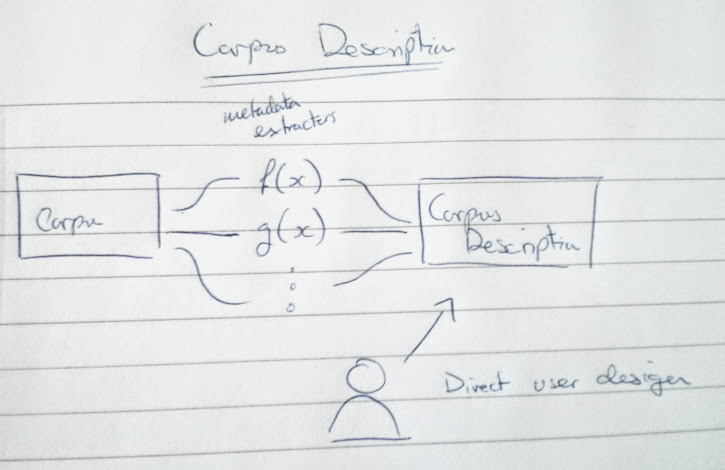
\includegraphics[width=0.8\textwidth]{rebuilding/profiling}
    \caption{Creation of a corpus description}
    \label{fig:rebuilding:profiling}
\end{figure}


The process of building a corpus description is outlined in~\ref{fig:rebuilding:profiling}.  For direct use, the user would specify their salient dimensions, and the distribution for each.  This is essentially a description of the sampling policy---where variables are discrete and nominal (such as genre labels), this would take the form of a table with desired proportions against each.  Where variables are continuous, a probability density function is defined.  Note that this method does not, without prohibitive complexity, allow for specification of interactions between variables\td{return to this and comment on it later}.

Profiling through the use of a `seed' corpus begins with specifications of the salient dimensions, the data for which are then read from the seed (by $f()$ and $g()$ functions in the figure).  As each document is read, the corpus description may contain information not only on marginal distributions for each variable, but also the effects of conditioning on one or more value.

Note that, whichever method is used, this stage is merely a metadata description task.  The corpus description document itself contains no more information than the metadata of the corpora from which is it built---indeed, where all variables are both external and nominal, this reduces to a simple table of frequencies for each desired value.  

Those specifying variables to describe must, as with all sampling, be mindful of their potential systematic correlations with variables of interest to any given research question.  The value of this approach is in documentation---it is possible for a researcher to eyeball the variables (and potentially their distributions) and determine whether or not a corpus is correctly conditioned for use inferring about a given variable.  This cannot be said for bootstrapping systems that use internal variables, which seek to copy corpus contents at the risk of varying their metadata.


% ---

\subsection{Retrieval}
Retrieval in accordance with the complex distributions specified in a corpus description is challenging in two ways:

\begin{itemize}
    \item Samples must be taken from the corpus description in accordance with a complex empirically-determined distribution;
    \item Any combination of variables sampled from the distribution must then be sought based on its metadata alone.
\end{itemize}

The former of these is difficult because many seed corpora may lack sufficient data to specify their distributions, and because of the high dimensionality of the distributions in question.  These issues may be addressed using techniques such as Gibbs, slice, or rejection sampling.  



\subsubsection{Resampling}

% \begin{figure}[h]
%     \centering
%     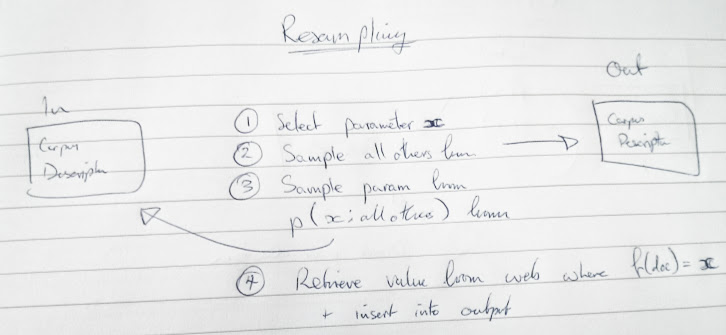
\includegraphics[width=0.8\textwidth]{rebuilding/resampling}
%     \caption{Resampling the corpus using MCMC methods}
%     \label{fig:rebuilding:resampling}
% \end{figure}



Resampling from the original corpus produces a `prototype' document, which has values of metadata fields that, over time, hold the same distribution as those in the seed corpus.

The process of constructing a new corpus is one of continually producing these `prototypes' conditional on the values of metadata already sampled, and then retrieving texts matching each.

To perform this resampling, we must be able to sample from a distribution proportional to that of each variable conditional on all of the others, requiring that the corpus description contains information on interactions between values.  As such it is only possible if the original corpus description document contains this information, something that is only practically a product of describing an existing set of documents (as manually filling in the values would be prohibitively expensive).


There are a number of methods by which this prototype document may be selected.  For the purposes of this study, two were implemented:

\begin{itemize}
    \item Simple selection from marginals.  This is the best case possible where a corpus lacks interaction information, and follows the joint distribution of the metadata properties across the whole corpus.  Despite its relative simplicity it may be suitable for some corpus designs, and is analogous to the BNC's balancing of spoken corpora \td{check this, cite the page where they describe their balancing}.
    \item Full conditional selection.  This is implemented by selecting a random sequence of metadata types, and then conditioning on a value drawn from the distribution of that type conditional on the values selected for those previous to it.
\end{itemize}

\til{Does this need the algorithm for both here?  It's terribly simple}

The former of these, whilst faster and simpler, will fail to take into account any interactions between metadata and is included since it is the only method capable of running on a very simply specified corpus description.  The experiments in this thesis use full conditional selection, as they have the luxury of using a corpus description built from a full seed corpus.



\subsubsection{Seeking the Prototype}
The main practical problem of sampling according to the original corpus' distribution is now framed as an information retrieval task.

This retrieval task is challenging on its own, but errors in performing it have specific ramifications for this sampling process:

\begin{itemizeTitle}
    \item[Dimensionality]As the number of metadata properties in the prototype increases, the search space from which a document must be selected increases exponentially\footnote{Or, strictly, somewhere between linearly and exponentially, if the metadata properties are not truly orthogonal}.  This has severe ramifications for rejection sampling techniques, which become intractable where the ratio of the search space to the area under the target distribution is high.

    \item[Selection of dimensions]Metadata types are selected for research reasons and do not necessarily correspond easily to existing online indexes or retrieval methods.  This means that even specifically seeking a document with one value of metadata may be a challenging task.

    \item[Error in selection]In part because of the above point, documents retrieved are unlikely to be a perfect match against the prototype.  Errors in multivariate selection will follow the population distribution conditional on those metadata values being sought: something that will introduce systematic (yet measurable) bias in the dataset\footnote{The one, extremely unlikely, exception to this is if the population distribution happens to be the same as the target.}.
\end{itemizeTitle}

The retrieval of a prototype, then, is limited to approaches that take into account not only the value of a metadata property to be sought, but also the nature of the source (in this case the internet) and any interactions that are likely to expand the search space to intractable proportions.  It should, of course, also minimise error in selection.


\begin{figure}[h]
    \centering
    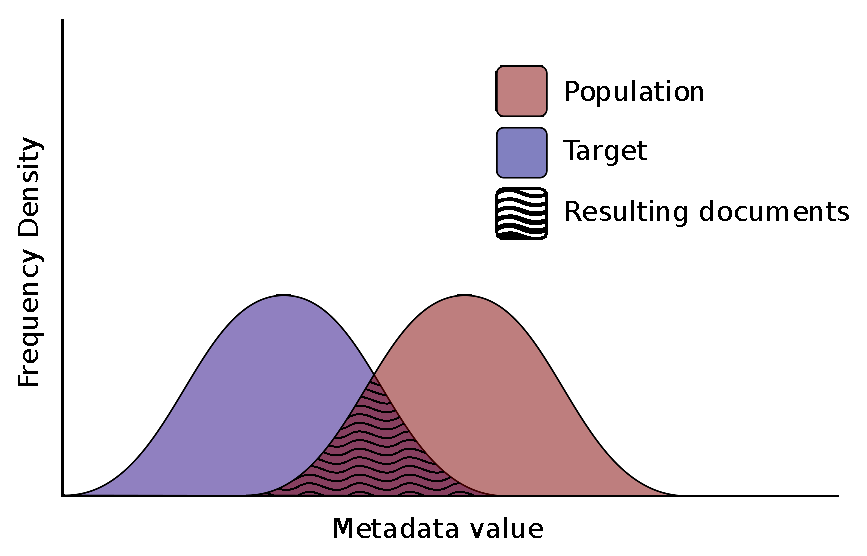
\includegraphics[width=0.8\textwidth]{rebuilding/population-bias}
    \caption{The influence of a biased population distribution on metadata selection}
    \label{fig:rebuilding:population-bias}
\end{figure}


In such a case that the retrieved document is a perfect match to the prototype, the output set of documents will converge to the target distribution.  If it is imperfect but randomly so, there will be an increase in variance in the output distribution.  If it is imperfect and the population is biased (or, in the worst case, does not overlap even slightly with the target), then the results will converge to a distribution with bias following the population distribution.  On Figure~\ref{fig:rebuilding:population-bias}, we rely on the black distribution falling within the red one.

The last of these is the product of an attempt to do something fundamentally impossible: the design of the system is such that this bias is measurable (and may thus be seen to be above some subjective threshold) rather than that it is eliminated for every scenario.  This bias is also evident in existing bootstrapping tools such as BootCaT~\cite{baroni2004bootcat}, however, they seek a looser form of coupling between input and output distributions so this bias often goes un-noticed (or, perhaps, desired\footnote{The comparison of distribution of seed terms to resultant type frequencies yields information about the search method and population, though these are conflated in the process}).

Instead of sampling a corpus \textsl{of} the web, we are sampling one \textsl{from} it, on assumption that the web is already a poorly-indexed supercorpus of documents that are diverse enough to satisfy the majority of research questions.  In terms of Figure~\ref{fig:rebuilding:population-bias}, we assume that the distribution in red has a very high variance (not just in one dimension as illustrated, but also in interaction with other metadata.  Clearly, the case in which this assumption is least strong is the replication of web corpora, and it is perhaps most strong for speech or other particularly specialist sources such as medical notes.

% ---
\paragraph{}

There are multiple possible approaches to this retrieval task, which mirror the web corpus building approaches of searching and sorting.  Each type of metadata may use one or many of these, depending on their relationship to the structure of the web.  They are listed here in descending order of 'direct applied expert opinion': the first item in the list relatively dispassionately seeks similarity, and the last uses human judgement directly to identify documents.



\paragraph{Searching}
\label{sec:rebuilding:design:searching}
Using similar methods to BootCaT and other seed-based corpora, it is possible to identify documents conforming to certain metadata values by using a search engine.  This encounters minor difficulties in that it is often necessary to transform an ostensive definition (e.g. the domain from which a text is drawn) into an intensional one (i.e. some keywords or other features typifying the domain) in order to fit the format desired by search engines.

If the method detailed here is used only for metadata types which are retrieved by example (the intensional definition above), then this technique for document-seeking is functionally identical to BootCaT's approach.



\paragraph{Directed Crawling}
Another technique widely used in existing tools is crawling.  When downloading documents using a spider, it is common to identify the next set of links (the `fringe') and then select from the fringe using a suitability metric.

The problem of directing a spider is then one of relating the features visible about a link (link text, url features, position in text, etc.) to the value of a document that will be gathered.  This will often involve similar issues to the searching method: it is necessary to examine document content and compare it to some ideal of each metadata value in order to form the link.

Many spiders currently focus on document `goodness' by simple definitions of information content or URL features~\cite{schafer2014focused,ferraresi2008introducing}\td{cite 'big and diverse is beautiful'}---These produce samples that are designed to approach simple random samples (SRS) in order to approximate the population of sites over which they run whilst exploiting the hyperlinked structure of the web.  The approach required to deliberately skew this search is arguably easier than this: a spider may follow rules based on keywords or site features, rather than modelling the content of documents in great detail.

The starting point of each spider may itself be determined by using a search engine.  This is common practice, used to direct spiders to relevant starting points, however, the ratio of crawling/searching used for any given selection may greatly change the output.



\paragraph{Existing Indices}
The use of existing indices for certain types of metadata is a main technique used in conventional corpus construction.  Online, however, this avenue is often neglected (with the notable exception of WebCorp~\td{renouf2003webcorp} and Barbaresi's examination of indices as seed URL sources~\cite{barbaresi2014finding}) despite the existence of many subject-specific indices and general-purpose manually-curated web directories.

By aligning the taxonomies used in metadata to those in an existing web directory, it becomes possible to use the contents of the directory to access documents authoritatively categorised by humans (or to start crawling from these).

This method is subject to errors regarding the age of content on web directories (whose popularity is waning in favour of search engine technology), as well as those introduced by human categorisers whose aims may not be aligned to the definitions required for a given research question.  Additionally, the granularity of each category is fixed and cannot reasonably be changed.

Nonetheless, such an approach is close to that used in conventional corpora and is easily defended providing that the directory is well trusted.
\til{Note that 'best of the web' has a specific blog directory and is used by search engines}

\paragraph{Crowdsourcing}
Crowdsourcing services offer a cheap mechanism for retrieving documents by requesting that humans manually seek a document fitting the prototype metadata.  This method has severe volume and speed limitations not present in the others, however, the accuracy of a human search is likely to be far greater, minimising overdispersion in the output set.

Where a corpus must be duplicated as accurately as possible (yet there is less importance placed on scale or speed of rebuilding), this is most likely a good choice for almost all metadata properties.

The major disadvantage of this method is that the speed of lookup is greatly reduced, bringing the corpus building process closer to that used by a conventional corpus.  The main difference here is that the weight of expertise required to select documents is handed off to those constructing the corpus definition, rather than those searching the indices.







\subsubsection{Candidate Selection}
The process of running heuristics will return a set of candidate documents, each of which will be returned under the condition that it satisfies the metadata property that each heuristic is designed for.  The size of this set is dependent on the probability of error, and is discussed below in Section~\ref{sec:rebuilding:design:minerr}.

Since each retrieved document may be missing metadata in some dimensions, it is necessary to infer the values for these from the document itself.  This process may use external variables such as HTTP headers/meta-tags in the header of the document, or internal ones that are assessed using some measure unrelated to the variables of interest to those constructing the corpus.  This process is heuristic-dependent, and may be thought of as an inverse function to the above.

Documents may be ranked by similarity in vector space only after normalising each metadata distance metric (otherwise, distance metrics liable to output large numbers would be apportioned a larger importance in overall fit).  This method also allows imposition of weights to specify which dimensions must fit more accurately.


\subsubsection{Iterating to Minimise Error}
\label{sec:rebuilding:design:minerr}
It is necessary to iterate an arbitrary number of times to retrieve a full corpus.  If each prototype document is matched closely, a simple repetition of the above will return a corpus that converges to the desired distribution, however, as mentioned in~\ref{?}, this approach may incorporate bias from the population.

There are two possible approaches to working with biased populations:

\begin{itemizeTitle}
    \item[Feedback from output to target distribution] Adjust the target distribution to reduce the probability for those documents already selected.
    \item[Rejection sampling]  Select a large number of candidate documents and then identify the document (or subset of documents) that best fits the prototype
\end{itemizeTitle}

The former of these approaches may seem ideal, however, it will only be effective if sufficient documents have already been selected for each conditional distribution, and if the population distribution is only slightly biased.  It will also slow down the seeking stage of each document and, in the event that the population yields no perfect documents, stop it completely.  It is a stricter and more reliable approach, but also vastly reduces the practicality of any system using it.

Variations on this theme form the basis of many MCMC methods, particularly Metropolis-Hastings.  MCMC algorithms are generally used where it is difficult to estimate marginals, however, this is not the case for our corpus data.

\til{Check that there isn't some way these can be used... [DL]}

The latter, rejection sampling, is much more viable, as the clustered and hyperlinked nature of the internet makes retrieval of many similar documents only slightly more difficult than retrieval of just one.

The [hyper-]volume of the search space increases greatly as dimensions are added.  This is largely mitigated by the directed document hunting approach above, which seeks to minimise the distance between each dimension's sampling distribution and the target.  Simply, the better the heuristics are (measured in terms of precision/recall), the more tractable any selection is and the fewer documents that need selecting.  The number of documents that needs selecting is proportional to the ratio of the areas under the joint ditstributions of the PDF of the heuristics' selections over those of the target distribution.

$$
numdocs \propto \int{\prod{heuristics}} / \int{\prod{target}}
$$
\til{revise the above to be more rigorous}

Where a target is defined in terms only of its marginals (as is likely when constructing a corpus from scratch), the interactions observed will be defined by the population of documents online, and the sample will exhibit conditional distributions that are peculiar to the internet regardless of its marginal distributions.  This approach relaxes the original sampling criteria applied to the seed corpus too, making replication far simpler at the expense of any best-effort approach to minimising bias across multiple dimensions.\td{ahrg}

As the population distribution for each heuristic is unknown (especially if they include interactions), it is impossible to know to what degree it is being undersampled.  This is another source of bias, however, it is one that is clearly labelled as such: those using a heuristic would do well to know its theoretical underpinnings and the methods it uses to select data (just as any corpus user should read the manual).

The main benefit of rejection sampling is that we are able to degrade the performance of the algorithm gracefully.  If, having sampled $n$ documents, we wish to relax the conditions of a match with the prototype, this will have only a minor effect on the corpus (increasing its variance and applying a small bias in the direction of the difference between the population and target modes).  

The degree to (and conditions under) which this relaxation occurs must be determined according to the particular demands of the application for which a sample is being built.



\subsection{Measuring Fit}
A system built with contingency for accepting certain levels of error is of very little use without some method for measuring it in operationalisable terms.

A number of properties of the system are measurable, each yielding information that is useful under different circumstances:


\paragraph{Heuristic Quality}
The quality of each heuristic may be measured according to its ability to return documents satisfying the one metadata value it is seeking.  This may be expressed in terms of precision and recall, or an aggregate thereof such as an F score.

\til{Blather on defining those things?}

The choice of evaluation metric will vary according to the type of metadata and its availability online.  Heuristics operating in particularly large search spaces (such as those primarily using search engines) will desire a greater weight on precision, whereas those seeking rare (online) data will favour recall.  Since heuristics are, ideally, already the results of well-established methods in linguistics, this score and its desirable range should be established empirically prior to use.

The F score may also be generated only for the best documents returned, providing a score for the whole `batch' of documents returned by a heuristic.  This measure is likely to be more representative of stateful heuristics (i.e. those that crawl), however, it conflates the statistics used for measuring document similarity with those used to retrieve them.

Ideally, heuristics form pluggable, reliable modules with known degrees of error that may be ignored when using the method as a source of linguistic data.\td{yeah, right}  The degree to which this applies is defined by how well each is aligned with a source of data: Keyword-based heuristics, for example, are well aligned with the search systems of search engines, but poorly aligned with the strengths and weaknesses of humans seeking a document type.

The value a heuristic yields is a trade-off between how closely it describes the document and how accurately it is possible to retrieve a document from the source. \td{perhaps remove, poorly worded}


\paragraph{Document Distance}
It is necessary to identify differences between documents' metadata values both in order to select them from the set returned by each heuristic and to identify overall deviance from the target distribution.  The former is computed after documents have been retrieved by a heuristic but prior to their selection; the latter after selection.

Binary selection criteria (are the metadata in this document the same as another) offer a way to guarantee convergeance to the target distribution.  They are an ideal case which will be tractable in only certain circumstances.

Relaxing the similarity requirement requires a finer-grained distance metric for each metadata value.  The distance for each candidate document may then be measured and a `best fit' selection made.  Alternatively, upper bounds may be set on suitable distances from the prototype for each metadata type, leading to selection of all documents which satisfy those criteria.

Having selected candidate documents using heuristics, it is possible to estimate and then sum the distance each has to its intended value from the prototype.  The sum of squares of each of these will result in the overall error for the target distribution, being analogous to the mean squared error:

$$
MSE = 1/n\sum_{i=1}^{n}\sum_{d \in D}^{d}{(P_i^d - C_i^d)}
$$ 

Where $P_i^d$ is the value of metadata type $d \in D$ of prototype document $i$, with $C$ being the equivalent selected document that was ultimately added to the results set.  $n$ is the number of documents selected.




%\sepline






%\til{

% ---
% * Break into dimensions, search, use rejection sampling
% * Select a subcorpus from the target, break into dimensions, search/spider, use Viterbi to balance biases
% * Feedback from output corpus to subtract from target corpus (sample prototype from difference)
% * Send to AMT for manual selection of a document
% (* Use PCA to derive similarity score)
%}









%
%Resampling according to multivariate distributions is possible using Gibbs or slice sampling, both of which are MCMC techniques---the `output' distribution of prototype metadata will iteratively approach the distribution of input data.
%
%This process is nonparametric, and thus able to accept arbitrary empirical input distributions and arbitrary modifications thereto.  This allows us to arbitrarily boost the sampling probability of a given category, or to ensure that variables with hitherto-unseen values are considered contributory to the output corpus.
%
%Gibbs sampling is also commonly used to infer the posterior distribution of individual variables by fixing the values of the input distributions.  Though beyond the scope of this thesis, it would be possible to use this technique to fix input variables and identify the distribution of metadata values also described in the corpus description document.  This technique would be highly sensitive to the bias of the retrieval mechanism, and would require a particularly large seed corpus to operate meaningfully.
%

%\til{
%Theoretically speaking, the corpus is reconstructed as a distribution of all internal variables on the document, conditional on the values in the metadata.  So long as the retrieval engine can find documents fitting the distribution of input data, the output data will conform to the posterior distribution of word frequencies (or any other internal property one wishes to reason about).

%Separation of the latent (internal) variables into a block is consistent with a 'block gibbs sampler'.  Ignoring them as a block is consistent with a 'collapsed gibbs sampler'.

% This is awesome: http://www.people.fas.harvard.edu/~plam/teaching/methods/mcmc/mcmc_print.pdf
%}


%\til{ Describe gibbs formally, and compare slice to it.  Describe the process of resampling from the output using the input distribution. }












\section{Method \& Implementation}
\label{sec:rebuilding:method}
As this case study is exploratory, seeking to drive and refine the methods used for recording \textsl{all} language use, an iterative design was chosen.  This saw a number of preliminary sampling periods, with a review after each to identify the strengths and weaknesses of each.

The subject was myself---this was done for a number of reasons:  Firstly, legal and ethical issues surrounding recording and review of the data were mitigated by having the analysis performed by a member of the original conversations.
Secondly, iterative review of methods involved was possible with internal, `white box' examination of how data were collected, and what edge cases and procedural difficulties arose.
Thirdly, the demographic status and other person-related variables are well known and need no formal elicitation, minimising time spent on construction of questionnaires etc.


\subsection{Data Sources}
Before the first iteration of the sampling/review process, all of the possible language data sources used in everyday life of the subject were informally identified.  It became clear that these data sources exhibited properties that would make sampling easier, or less intrusive.  They were classified by the methods required to capture their text:

\begin{itemizeTitle}
    \item[Persistent] Resources that exist in a format that is immutable and easily retrieved.  This covers many physical items such as books, and some broadcast media as well as notes made in a notebook.  Only identifying information must be stored during sampling itself, in some cases merely an ISBN or similar index code.
    \item[Ephemeral] Language data that cannot be accessed after-the-fact in any way, or may differ by time or context.  This most obviously contains speech, but also many websites, things such as billboards that cannot be readily accessed, or todo lists that get destroyed.
    \item[Digital Origin] Documents that are read, or written, on electronic devices.  These may fall into either of the above categories, yet as they may usually be copied with no overhead, it is often simpler to store them at the time of use.  Many document types are now digital, as well as the obvious sources such as email or online chat.
\end{itemizeTitle}

This classification was useful in order to minimise the intrusiveness of a collection method, whilst maximising the detail recorded for a given source (ideally to the point of storing verbatim text).  In practice, methods were easy to develop for automated recording of digital documents, and many techniques exist for sampling non-digital persistent and ephemeral sources with scientific levels of accuracy already.

Sources initially identified by introspection are listed in black in Figure~\ref{fig:personal:datasources}.

\begin{figure}[Ht]
\centering
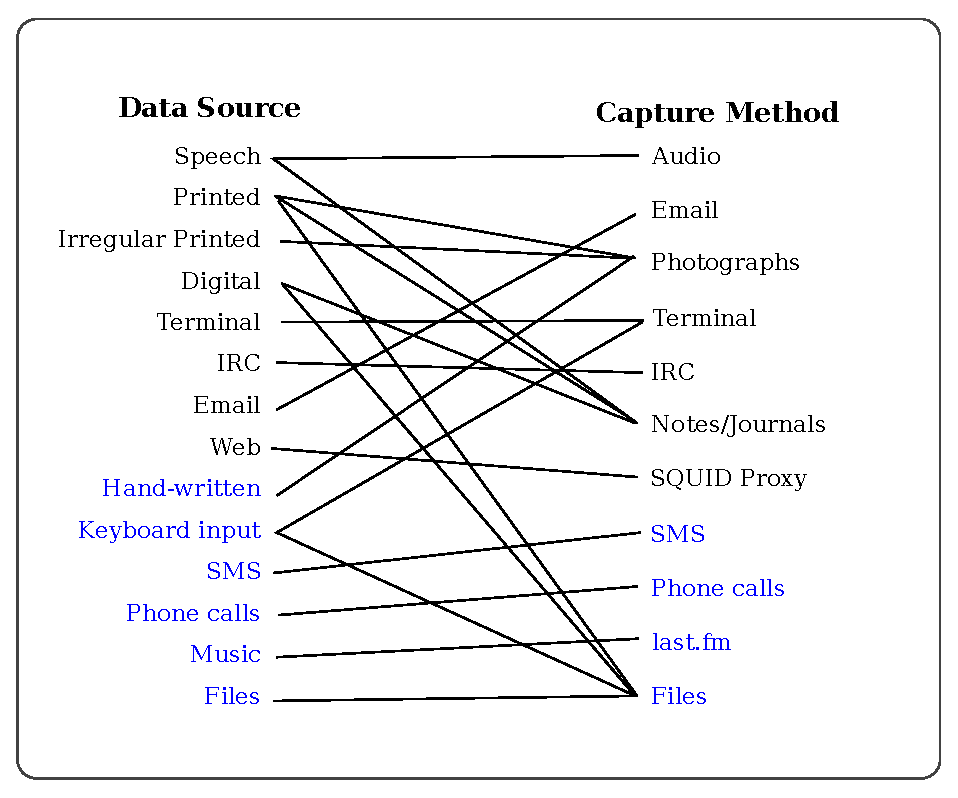
\includegraphics[width=0.7\textwidth]{personal/sources}
\caption{Data sources and their appropriate capture methods (those in blue were added during preliminaries)}
\label{fig:personal:datasources}
\end{figure}



The inadequacies of introspective methods to comprehensively identify data sources soon became apparent during preliminary tests, as the process of recording brought increased awareness of language use, raising a series of edge cases.  These were collected and used to augment the list of sources shown in Figure~\ref{fig:personal:datasources}.  As well as covering the set of sources to be gathered, methods of collection were chosen with flexibility in mind in order to cope with un-envisaged sources of data\footnote{This flexibility has the unwelcome effect of slowing down analysis later on, and may be undesirable in some use cases}.


% \begin{itemize}
%     \item Speech
%     \item Printed documents (i.e.\ letters, brochures)
%     \item Digital documents (same, but unprinted)
%     \item Terminal logs
%     \item IRC logs
%     \item Email
%     \item Websites
%     \item Unusually formatted printed material (posters, labels, advertising on vehicles, billboards, etc.)
%     %---
%     \item Written (but non-OCRable) material
%     \item Key strokes
%     \item SMS records
%     \item Phone conversations (separated from speech as they yield differing metadata)
%     \item Music tracks
%     \item Files accessed
% \end{itemize}

The list is necessarily furnished according to the life of the subject in question---from this study I am unable to assert that it is generalisable to others, though the process of doing so would involve relatively little intrusive sampling.

Each of these sources is `covered' by one or more sampling tools.  These tools progressed most during the iterative process, and each was subject to a number of procedural subtleties that were refined throughout the study.










\subsection{Recording Methods}
Methods used to record data were chosen for a variety of reasons.  They must, in sum, cover the sources mentioned above, be unobtrusive both for the subject and those around him, and be sufficiently flexible to cover unforseen contexts and data sources.

These methods can be separated further into two groups: many methods are capable of recording multiple sources, and serve to form a narrative that describes the metadata of a linguistic event, pointing at another source for the data itself.  These methods were chosen to allow for post-hoc sensemaking and narrative creation, something that was added to the experimental procedure after the first iteration indicated how difficult to operationalise much of the data would be.

The second set of methods are focused on a single data source, typically requiring little to no manual intervention to record data.  Their records are either indexed by time, or by the more flexible methods mentioned above.


\subsubsection{Indexing and Overview}
\paragraph{Journals and Note-taking}

\begin{figure}[Ht]
    \centering
    \includegraphics[width=0.8\textwidth]{personal/notebook}
    \caption{The live notebook}
    \label{fig:personal:online_notebook}
\end{figure}

Two journals were maintained throughout the sample.  The former of these was an A6 notebook maintained `live' as events occurred (pictured in Figure~\ref{fig:personal:online_notebook}).  This was used to store durations of conversations, titles of persistent sources, etc.

The second was a nightly (`dead') journal, maintained at the end of each day in a narrative style.  This blog-like record was intended to reflect in depth on the proportions of text used in each source, and how attentively each linguistic event was engaged in.  The writing of the journal itself was not logged by any other methods.  It was also possible to attach daily records to this journal, and the process of writing it inserted an opportunity to reflect on the mnemonic codes used during the day.  This process is described in context in Section~\ref{sec:personal:method:recording}.

The live notebook proved to be the primary indexing method for all other sources of data, and its maintenance was the primary overhead of the study.  As illustrated in Figure~\ref{fig:personal:notebookformat}, each entry in the notebook was eventually reduced to a compressed form that roughly followed one-line-per-event, storing the time each event occurred, any identifying information deemed necessary for later memory of it, and a duration or other index of word counts.

\begin{figure}[Ht]
    \centering
    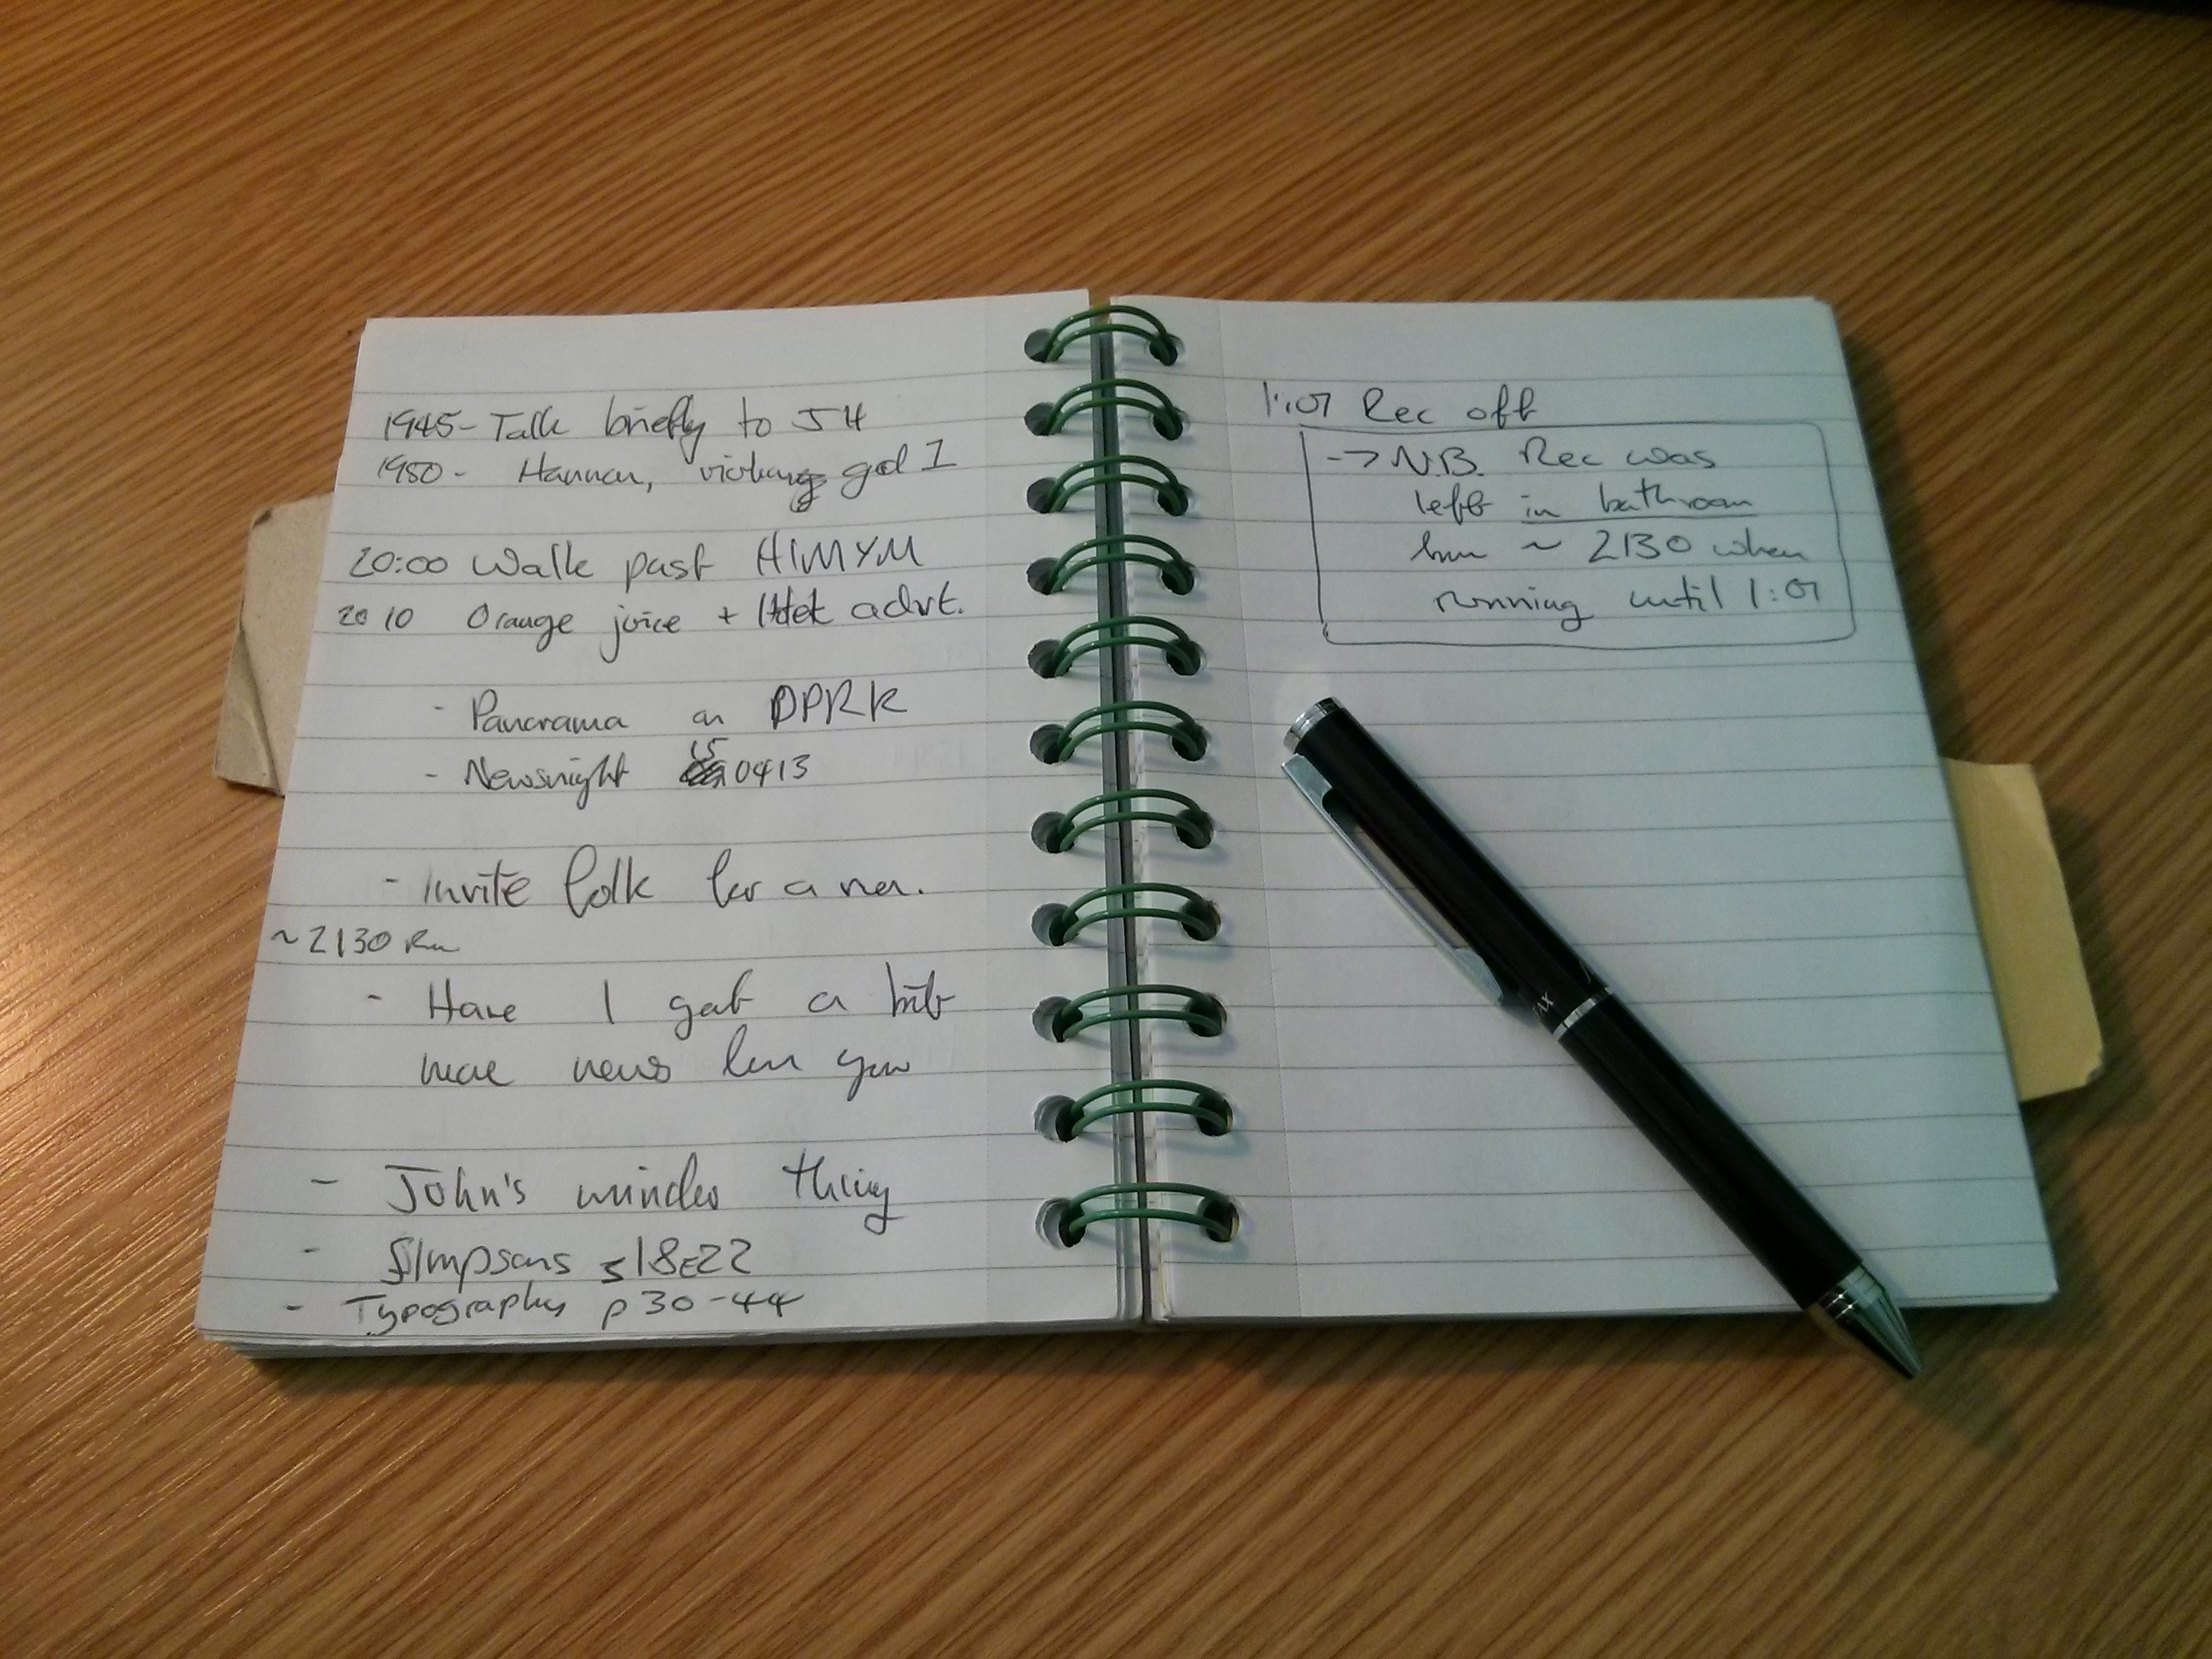
\includegraphics[width=0.8\textwidth]{personal/notebookpage}
    \caption{A page from the live notebook, detailing the format used}
    \label{fig:personal:notebookformat}
\end{figure}


Problems of simultaneous events and split attention were solved in the notes by having a start/stop event for ongoing events, and by using the nightly journal to reflect upon each event.

\paragraph{Audio Recording}
Following work on machine listening, the original intent of audio recording was to capture the occurrence and duration of conversations, as well as any smaller interactions that would otherwise be difficult to capture (such as greetings, thanks when opening doors, etc.)


\begin{figure}[Ht]
    \centering
    \includegraphics[width=0.8\textwidth]{personal/dictaphone}
    \caption{The audio recorder used}
    \label{fig:personal:audiorecorder}
\end{figure}



Capturing was performed with an Olympus VN713PC dictaphone, storing audio on a suitably sized external card that yielded many days' continuous recording.  Provision was made to download recordings each night and store them with the nightly journal, however, in practice they remained on the recorder until the end of the study.


\begin{figure}[Ht]
    \centering
    \includegraphics[width=0.8\textwidth]{personal/clicker}
    \caption{The second audio index marker}
    \label{fig:personal:clicker}
\end{figure}
% \FloatBarrier{}

Aligning the recorder's output to the events mentioned in the notebook was a tricky process---Though the recorder itself supports index marks, there is a limit of 99, which was deemed too low for continuous use.  Two devices were built to insert absolute silence onto the recording (something that is rare in real life and thus easy to programmatically detect), the later of which is pictured in Figure~\ref{fig:personal:clicker}.  These clickers were to be pressed at the beginning of each conversation, so that voice activity detection could be performed to estimate the word count of each conversation (or, in an ideal world, extract verbatim text).

In practice, the process of tapping the button proved intrusive and, from the perspective of one talking to the subject, suspicious.

The mechanism used for the final iteration of the study was far simpler---the recorder's start time was written in the live notebook, and entries therein were keyed by computing the offset between the two times.  Though this incurs a minor overhead in coding the data, it also allows for spontaneous conversations without much overhead, something that is particularly important to the study of text type proportions.



\paragraph{Photographs}
The primary method of capturing ephemeral, irregularly formatted, non-digital texts was photography using a cameraphone.  This method was chosen largely because the ubiquity of smartphones in British society has led to a situation where photographing fairly mundane items is widely unquestioned.

The smartphone used, a Motorola Milestone, also stores time and location data in its photographs using EXIF tags (as well as storing photographs sorted by day).  This metadata meant that there was often no need to file an entry in the live notebook, and the cameraphone could simply be used in a very unobtrusive ad-hoc manner.

In earlier iterations of the study, it became apparent that the loud shutter noise made by the Android operating system when taking photographs was problematic.  Though photography of signs, packets and such remained unchallenged, the attention of people nearby was drawn to the `weirdo with the cameraphone' all too readily.  This was solved partially (and with great difficulty) by disabling the noise, though it was still apparent from posture when a photograph was being taken.

There are notably a number of products available that continually take photographs for the purposes of life-logging.  These were considered for the study, but their aims are generally to capture each event, rather than specific aspects of selected scenarios.  The ability to consciously specify that the subject was more attentive in some situations (and take pictures accordingly) was judged to outweigh the value of having a continuous record (something much more capably performed by the journals).




\subsubsection{Targeted Methods}
\paragraph{Phone Calls \& SMS Messages}
Both of these are automatically logged by the Android operating system used by the subject, and each was also indexed in the live notebook.  The data was extracted using a free application that exported to XML.


\paragraph{IRC}
IRC was logged by construction of a bot.  This bot accompanies the subject into chatrooms and logs all messages observed, applying a rough human interest model to ignore data encountered when the user is set to away.


\paragraph{Web}
The SQUID webproxy was configured to log all traffic, and a number of logins were provided---one for each of the subject's internet-enabled devices.

The logs from SQUID store all requests, including advertising/tracking calls, downloading of things never read by the user (i.e. CSS and Javascript) and AJAX calls to partially reload pages.  As such, a large amount of processing was necessary to extract URLs from these logs, and to parse the resultant data into a usable format.

\paragraph{Keylogging/Terminal recording}
Terminals and keyboard input were logged using a custom application that wrapped a terminal, recording the time each character was sent or received to/from the shell.

Each terminal created started recording to a new log file, storing the time at which it was started and a series of offsets from this time.

\paragraph{Last.fm}
In earlier iterations it was apparent that lyrics in music were being missed as a source of text---all devices capable of playing music were configured to `scrobble' to the last.fm music service during the sampling period.

Though last.fm do not make their data freely available for access, third party tools exist to scrape their website and download detailed logs of tracks listened to.

\paragraph{Files}
Files were identified in a number of ways.

Some, particularly those on which the subject worked and contributed data, were written down in the journals.  This is a precise method of separating what has been read, but incurs a large overhead.

Since the subject works entirely on projects and files that reside in a repository managed by a Revision Control System (RCS), the logs from each commit were used to generate a diff, and this was accessed after the sampling period to identify contributions made.

Another policy that may be used is identification of files by unix mtime (modification) or ctime (inode change, often creation), however, this is fraught with inaccuracy, as files are liable to be modified on disk many times whilst being edited, and sampling the differences is likely to happen at haphazard times.  Further, this technique would capture many log files and others that have been edited by processes where the subject was not involved linguistically.  By contrast, commits to an RCS are scheduled around logical additions, and are manually pushed so that only deliberately edited files are stored.

Files uploaded whilst on other systems may be uploaded directly to the nightly journal, or stored on a flash drive that was carried specifically for the purpose.  In practice this did not occur during the recording period, though experience suggests these contingencies would be necessary if a longer sample were taken.

\paragraph{Email}
Emails are, again, stored automatically with sufficient metadata as to make them self-documenting.  However, rather than presume all were read in a given day, each was tagged after being read with a label corresponding to the day.

At the end of the sampling period, these tags were collected and downloaded in mbox format, whence they were processed by the operationalisation script.









\subsection{Recording Procedure}
\label{sec:personal:method:recording}
The study is based around a period of continuous sampling using the methods discussed above.  For two weeks (in some cases longer), data was captured for each source.  This process was structured around a daily routine:

Upon waking, and before any language was used, the recorder was turned on and a note of the time at which this occurred was made in the live notebook.  Recording was then continued until the end of the day without interruption.

The live notebook, smartphone, and flash drive, were carried at all times.  Since each of these could be backed up (the smartphone even did this backup automatically), the most data at risk was a single day.

Notebook entries were made as soon as was possible without interrupting the linguistic event being recorded.

At the end of the day (immediately prior to sleep), a journal entry was written in the nightly journal, and SQUID logs were uploaded for the day.  This journal entry forms a narrative, estimating the time taken and attention paid to items in the live journal for that day, as well as detailing anything that may be written in shorthand-mnemonic form.










\subsection{Operationalisation, Processing and Analysis}
\label{sec:personal:method:operationalisation}
Normalising and operationalising such heterogeneous data without large overheads proved to be a significant problem that was only partially solved, and the data set presented here required manual editing that was possible in part due to the fact that the analyst is the subject.

This advantage, clearly, cannot be relied upon in other studies, and this part of the method demands most further study in order to define typical parameters for many processes that are dependent on human properties.

Two main processes were followed in data processing.  The former of these was aggregation and normalisation---each data source was collected and transformed into a one-event-per-line CSV containing a standard set of fields (the selection of fields used was modelled on Lee's BNC index\cite{lee2001genres} in order to facilitate comparison).

After this normalisation process was complete, data were manually annotated to complete any fields that were not stored in the original metadata.  This was largely an objective, uncreative task that simply demanded human reasoning capacity, but it is inevitable that some bias will creep in at this stage.

The second stage of processing involved coding text types and roles.  This task is altogether more flexible and subject to design errors and bias than many of the normalisation stages, and was thus attempted in a manner that was designed beforehand.  Since the aim of this study is, in part, to identify text types not seen in other corpora, following an existing taxonomy would necessarily limit the coding of any newly discovered.  True free coding, however, is likely to draw distinctions between text types that are not made in existing taxonomies, rendering them incomparable.

The process followed was a hybrid approach---data were freely coded by inspection of the texts, but this was done with deliberate prior knowledge of Lee's classification scheme.  The intent was to categorise texts according to Lee's scheme only in so far as they were deemed suitable by the analyst (who is also, lest we forget, the subject).

Though this approach was suitable for the aims of this particular study, it is difficult to advocate for any others using the sampling techniques described, and its use here should not be taken as such.

%---
\subsubsection{Human Interest Models}
Beyond coding, by far the largest single influence on the data recorded was the human interest model applied.  This was created in order to take into account two factors that had become particularly apparent (and notably do not apply in the same manner to conventional corpus designs, where many eyes may cover a whole document in sum):

\begin{itemize}
    \item Often, only small (usually predictable) portions of a text are used.  For example, I have \textsl{started} to read more books than I have \textsl{finished} reading.  Generalised, this means that even Brown-styled corpora should favour the start of their texts slightly when selecting excerpts.  Some media were more susceptible to this than others, and the automated normalisation tools were built with facilities to take this into account\footnote{Amazon have the ability to monitor which pages are read on their Kindle ebooks, meaning that they possibly have a large dataset related to this effect.}.
    \item Texts, especially broadcast media and speech, were often used whilst also accomplishing a non-textual task (or sometimes both at once, such as talking with the radio on in the background).
\end{itemize}

Both of these were noted in journals, and added to the processing toolchain---each data source's normalisation script contained a model to extract the portions of text that were read, and each row of the normalised data format contained an `attention index', ranging from 0--1, that served as a coefficient of the word count.

Though crude, this measure was able to produce approximations for word counts that were inline with the expectations of the subject.  It is recognised that this may not hold much scientific value to others wishing to replicate the study, and in general it is necessary to investigate the inter-person variability of these properties in order to create more generalised processing tools.


% TODO: perhaps a run-down of each annotation program?
\paragraph{Web logs}
The human interest model for web logging was built by inspection of the web logs and cross-referencing with information about the hosts identified.  The normalisation script is concerned primarily with removing material that was downloaded without ever having been viewed, for example, non-text MIME types and advertising, and contains a multi-stage strategy for excluding content:

\begin{enumerate}
    \item Filter only successful requests;
    \item Filter only those requests that are of textual mime types (\texttt{text/*});
    \item Apply a blacklist of advertising websites and file extensions (manually constructed);
    \item Discard links where the page was reloaded and the URL is the same as the previous entry in the list (this pattern is often caused by initially connecting to the proxy, for example);
    \item Discard Non-visible text items (non-body elements if the file is HTML), and remove markup.
\end{enumerate}

Beyond this initial normalisation, a speadsheet's \texttt{LOOKUP} function was used to manually assign attention coefficients to the domains, based upon entries in the journals and interesting portions of web pages that follow regular structures.

Days were classified as changing at 4am, since there were no points in the data set where the subject was still using the web at this time.



\paragraph{IRC Logs}
IRC logs were already stored using a limited attention model, which was based on the principle that, in IRC, conversations are started, live for a short time, then die off as people in the channel return to work.  The bot performing logging would start logging (and continue to log) for as long as the subject was talking, stopping 10 minutes after the final utterance.

In order to capture a human notion of day, that is, one demarked by sleep rather than midnight, the start time of each conversation was used to determine the day its data fell into.



\paragraph{Terminal [Console] logs}
Terminal data was logged with timestamps on each individual character, and the model was thus responsible for inferring when a command had output, and suggesting which portions of text were still on screen.

This was done with a `timeout' and a `scrollback'---the former describing a delay that had to be present for the text to have been read (rather than simply scrolling offscreen), and the latter describing the average size of a terminal (and thus the number of rows of text that remain displayed).

These parameters were tuned to match the specific data sampled over the period---for example, the recording period included terminal use displaying logs from software that was being developed, and these would produce thousands of lines of output before a pause.




\subsection{Coding and Genres}
Since the case study is in part aiming to identify genre distinctions not found in other general-purpose corpora it is not possible to select, a priori, an authoritative taxonomy of genres.  This problem is further complicated by the mix of spoken and written data in the corpus, something that would usually be more formally separated.

% \til{Also note how I'm coding things from both spoken and written, and such, thus one taxonomy would be unable to cover it anyway?}

Genre distinctions were made using a process that loosely follows the principles of the coding stages of grounded theory\cite{glaser1992emergence}.  
This involves a focus on free coding, and a consideration of all available context and information---something aided by the `memoing' innate in the design of the journals.  Free coding was performed with prior knowledge of Lee's genre categories.


This process was done in order to deliberately apply distinctions made by Lee where these seem appropriate, but to retain the flexibility to deviate where portions of the corpus did not fit comfortably within the existing categories.  This soft alignment was chosen in order to ease comparison against existing corpora, especially the BNC\@.  No effort was made to adhere to Lee's specification directly, so as to prevent forming a disconnect between the Lee-inspired categories and those that were sufficiently different to form their own.
% as this would lead to over-specification where the case study's corpus proves more diverse in form than the equivalent BNC category.

% It's particularly noteworthy here that the analyst selecting codes for genres is the same person as the subject gathering the data.  This, along with the mnemonic form of the notebooks and data captured, provides extra (informal) insight afforded by context.


Because of the large volume of data, and the manner in which it was extracted from its original sources, coding was performed using a semi-automated process on a source-by-source basis.  This was chosen in part because the source itself refers to how the language was used by the subject, rather than simply what form it was available to the corpus builder, and is thus a contextual factor affecting genre distinctions.  This would have to be documented in more detail for other studies.

For data that were processed and annotated largely automatically, codes were assigned after a systematic review of the data itself, using a spreadsheet to reduce the number of lines according to variables that were assumed to define a given genre (for example, web data was split by domain, and music was assigned by artist).  These distinctions were then written into the extraction tools as heuristics, or applied directly before being merged with the main corpus.

For data such as images and notebook entries manual coding was required.  This was completed using similar tools, except that it was seldom possible to reduce the data set before coding, and thus was not possible to apply heuristics to impute data.  Data recorded in these formats were often more varied with many unique or esoteric entries (such as the single tax disc\footnote{A format that now no longer exists after the UK's move to managing vehicle excise duty electronically.}).

In order to better align the informal genre distinctions with Lee's format, the final document genre distinctions were formed by prefixing the data source, i.e.\ transforming `rock' into `music/rock'.  These resultant genres are used herein for describing the corpus, as the basis for any direct comparison with Lee's BNC index.



% ---

This process of augmenting manual entries method would, if extended to use external data sources (such as the CDDB music information service\footnote{Now known as `Gracenote': \url{http://www.gracenote.com}.}), be capable of automatically assigning genres for a number of data sources, greatly easing the manual intervention required.  It is also likely that improvements in computer vision (such as Project Naptha\cite{naptha2014homepage}), or applications of existing databases (such as Wikipedia, or the web itself) could be used to extend these methods further to cover images and other data that were manually processed here.



\section{Summary}

There are a number of methodological challenges that continue to prevent application of the methods described here to larger populations.  These are either due to the problems inherent in sampling varied data in the first place (digitising photographs or transcribing audio), or the processing required to transform data into a usable form (models of attention).

It is hoped that further work will be able to develop these methods in order to mitigate these issues, at least for certain applications.  However, the utility of these methods to the thesis is retained under less ambitious conditions of restricting a combinatino of the domain (for example, only sampling web histories or work-day language use) and the population (i.e. only people very similar to myself).

The practical issues encountered during sampling are largely minor, and modern portable technology proved decisive in making capture of hitherto-unseen (or at least widely ignored) sources of text possible in-the-field.  The census design lends an empirical justification to inclusion of these genres in larger general-purpose corpora, however, we are unable to formally generalise with confidence to demographics other than that of the subject covered.

Of particular note (and perhaps greatest generalisability) is the number of words used throughout the sampling period.  Almost a million words were input and output by a single individual over a two week period.  Since it is reasonable to deduce that this sampling is at best representative only of a normal working week for a single individual, it is rational to suppose that a corpus purporting to cover the whole population of a country demands a sample size far greater than many existing corpora.


This would seem to form an argument that it is simply not cost-effective to build a conventional general-purpose corpus large enough to represent large populations, suggesting that the focus should lie in those built for more specialist purposes, or those sampled non-probabilistically.  Here, the extreme size of web corpora may be well justified, so long as they can be shown to have been sampled rigorously.


This suggestion is reinforced by the obvious variability in the proportions of texts taken from each source, which will vary greatly by lifestyle.  Indeed, it seems that the measure of one's lifestyle by text source is a particularly direct way of characterising inter-person variability, and further work may be focused on this problem as a way of simplifying the methods described here.


Of interest to this thesis is the high level of detail that may be captured using this method.  The census design affords full coverage of a given area about which we may wish to generalise, and the detail it is possible to capture this way makes the data ideal as a `seed' for constructing larger corpora with comparable properties.  Application of these methods, as well as those using auxiliary data mentioned above, will hopefully render this sampling method a complementary one, to be added to the collection of existing corpus designs.

\til{Link back to main themes of thesis}




\chapter{Evaluation \& Discussion}
\label{sec:evaluation}
\section{Introduction}
Assessing the degree to which a sample represents the ground truth is an inherently difficult task, and one which is typically performed by comparison against `known good' data, or through the use of heuristics and checks involving reasoning about the world.

These strategies are particularly challenging for corpora, as linguistic data is both high in dimension and complexity, and the population being sampled may be vast.  In addition to this, corpora are so large that they are not practicably readable by a single person, and are difficult to qualitatively summarise or observe in an overview context.

Approaches available to corpus linguists centre around feature extraction and comparison, or evaluation for a given task.  

\til{ more, cover human comparison using sampling / triadic stuff }





\section{Method}
\subsection{Assessing Bias}
\til{The problem of establishing a measure for bias, especially in such hugely-dimensioned data}

\subsection{Similarity Measures}
\todo[color=blue!20, noline]{WHEN}
Discuss the problem of evaluating a sample that has a gazillion dimensions, outline why a linguistic approach was chosen (and which one[s]).







\til{The below are aligned with habeas' use cases outlined in `repeating'}
\section{Corpus Dissemination}
Homogeniety of corpora built from the same CDL across various likely conditions, such as [web] location and time.


\section{Corpus Construction}
Similarity of a corpus to its CDL, as determined by humans.  This is, in a way, also a test of the ability to construct personal corpora (such that the proportions and CDL properties are taken from a 'seed' corpus).







\chapter{Conclusions \& Review}
\label{sec:conclusions}

% Summary

This thesis has examined the problem of improving corpus sampling from a number of perspectives.  This chapter will serve to summarise these, before offering an overview of significant areas for further research.

Chapter~\ref{sec:longitudinal} presents a motivating study of link rot in open-source corpora, finding large variations in document half-life using a URL-seeking method.  This illustrates that temporal effects have a significant impact on the availability of data, and that such effects vary according to source.  Much literature exists that has related these to layout features (such as the role of navigation and landing pages), yet the impact this has upon linguistic content is less well understood.

In order to make such investigation possible, a cohort sampling approach is necessary, performed at a high resolution over a long period of time.  The LWAC tool automates this process, providing a mechanism to construct large-scale corpora that are indexed by time as well as URL.  Key to the utility of such a tool is its performance, which was shown to be adequate to construct corpora in the millions of documents, sampled daily.

This wealth of data enables analysis not only of `simple' availability, but also changes through time due to editorial processes or site redesigns.  This may allow sociolinguistic analysis surrounding specific events, or a more general picture of long-term language change through time.  It is hoped that the latter of these can be used as auxiliary data to inform stratification of future general-purpose corpora (or at least their web-based components).

% ---
Chapter~\ref{sec:personal} presents a case study detailing a short-term linguistic census of a single subject.  The sample design used therein is a `narrow and deep' design, orthogonal to the 'broad but shallow' coverage of the large national corpora.  This makes it particularly useful for judging rationally how well such data apply to individuals, and offers a way to retrieve metadata not found using conventional data gathering methods.

Such a detailed sample also provides a mechanism for reasoning about corpus size: the data observed in just two weeks for a single subject yielded almost a million words.  Assuming significant inter-person variation for a given linguistic feature, this implies that a population of ~60 million people cannot be well represented by a corpus of just a few million words.  Quantitative knowledge of inter-person variation is needed to operationalise this, but such data could be gathered using some of the automation methods presented.

Such methods were largely taken from lifelogging, a field chosen due to its focus on unobtrusive, best-effort, and wide-ranging sampling techniques.  These proved to be significantly more troublesome than expected: though automation was assistive, much manual correction was necessary to operationalise the data, including the need for a human-interest model to correct summary statistics that were gathered at a low resolution.

% ---
Chapters~\ref{sec:rebuilding} and~\ref{sec:evaluation} cover a method for `profiling' a corpus purely based on independent variable specification.  This profile has many potential uses, both as human documentation for a corpus and as a machine-readable descriptor.

This system is one designed to extend and generalise the approach taken by BootCaT in order to make its selection criteria easier to operationalise.  It is designed to be modular, allowing those building a corpus to re-use algorithms and taxonomies in a simple manner: essentially, the aim is that the tool should be working using the same concepts and distinctions as the desired sample design.

Monte Carlo techniques were used as a method for operationalising the profile, something that was shown to achieve convergence to the desired distribution within a tractable period for a BNC-like corpus of written text.  The classifiers required to identify documents for final selection were shown to be workable, but their performance was borderline for the more complex dimensions such as genre---this is in part due to the ambiguity in the test data's taxonomy, and in part due to the difficulty of large-scale classification tasks.  Such issues are of wide utility, however, implying that improvement in this area will not require specific study.

Retrieval of documents according to the prototypes was shown to be possibly the biggest challenge.  This is in part due to the classic corpus sampling problems of being unable to locate documents in a uniform and reliable manner, and in part due to the biases seen online.  A number of methods were presented to work around these issues, such as manual selection or use of manually-curated web indices, and evaluation of these remains as further work.




% --------
\paragraph{}
To revisit the problem of representativeness, this thesis has taken the view that any such question must be framed in terms of a larger study design.  This is not to say that general-purpose corpora are impossible to create: sampling is such a challenging and resource-intensive endeavour that it will most likely always have to be offloaded onto a third party for larger populations.

The aim, then, is to provide a general-purpose corpus that is uniformly representative for a wide, and well-specified, set of research questions.  This corpus should be sampled using random sampling techniques, and this thesis' tools have been designed to inform stratification efforts with this in mind.  Such a corpus should also be unambiguously and comprehensively documented: assumptions should be made explicit in corpus documentation so that they may be compared against those made by researchers, and the limitations of the intended use of a corpus should be stated in quantitative terms.

The contributions within this thesis have been targeted to provide some insight into the underlying population that is not possible using current techniques.  I do not suppose that these alternative sampling designs will be used in their own right (though there is utility in this for some), but that the perspective they yield may be used to inform and improve upon existing corpus retrieval methods.


% Kilgarriff \& Grefenstette's issue with web corpora\cite[p. 343]{kilgarriff2003introduction}:

% \begin{quote}
% The Web is not representative of anything else. But neither are other corpora, in any well-understood sense.
% \end{quote}












% Further Work
\section{Further Work}
As much of this thesis has been exploratory, there is a wealth of further work necessary to maximise the value therein.  Whereas each chapter contains numerous notes in context, this is a high-level summary of the major avenues of inquiry.


% ====================================================================================
% \subsection{Further Work}
% Currently, workers in LWAC do not evaluate JavaScript or build a DOM (though they do send and receive cookies) --- increasingly these features are used by websites to display content, and extending workers to handle them broadens the set of pages it's possible to retrieve meaningfully.  Such an extension is expected to incur a heavy performance penalty, however, as it massively increases the work done by each client during downloads, and complicates the resulting data.

% The field of survival analysis offers a large number of techniques for studying the change in a cohort over time, however, this is largely focused on the existence of simple regressor variables.  This is suitable for technical properties such as those focused on by search engine designers, but less approproiate for digesting large quantities of text.  Techniques for time-series analysis of large corpora are developing, but are usually not based around a cohort-based design.

% The distributed nature of LWAC makes it possible to study geographical effects --- this is something that would require only modest outlay as virtualised infrastructure becomes cheaper.


% Further sampling and analysis is necessary to confirm the issues highlighted above.  This paper comprises a preliminary look at data sampled in a longitudinal study, which will go on to relate the influences of extrinsic document features (which may be used to inform sampling strategies) to their linguistic content.  

% This will involve, primarily, identifying the extent to which document attrition applies bias on linguistic content, rather than technical features, and how this varies through the sampling period.  Issues of particular interest include:

%





\subsection{Large-Scale Longitudinal Document Attrition Studies}
A large-scale longitudinal sample of WaC sources is one obvious extension to the work in Chapter~\ref{sec:longitudinal}\footnote{Indeed, one was underway, but due to technical failures the results were not ready for publication here.}.

Such a study would be able to answer questions not only on the rate of decay (as has been addressed elsewhere), but also the shape of the decay curve, hitherto presumed to be exponential for most types of data.

Further to this, there are many web page changes that do not constitute `link rot' in that the original information may still be present, but are still interesting for various linguistic and social questions, for example how often documents are changed in response to news events, or have their boilerplate changed in order to affect the context in which documents are presented.

Ultimately, developing a linguistic understanding of change through time will require significant work, however, a single large sample could provide useful information to those seeking to use large existing web or monitor corpora.

\subsection{LWAC Distribution}
LWAC's distributed design lends it particular powers in distinguishing web access issues from a geographical perspective.  With the low price of virtual machine rent, a network of LWAC clients could easily be constructed to access a number of websites from differing locations.

Such a configuration would reveal geographical changes made by site administrators for reasons of editorial control, censorship, and interference by service providers (Phorm\cite{clayton2008phorm}, for example).  This would open an avenue for investigation of a number of social factors, particularly as the (time-series) results could be compared and correlated with many real-world regressors, such as the incidence of political events.  Such approaches are already being widely used in social media analysis\cite{achrekar2011predicting,bollen2011twitter}, though the high number of societal covariates renders such studies difficult to validate.

\subsection{Slimmed-down Personal Corpora}
A natural progression of the work in Chapter~\ref{sec:personal} is the repetition with more subjects.  This is troublesome in part due to the in-depth coverage of language sampled, something that is likely to be less than critical for many research questions (such as those primarily concerned with `standard' day-to-day interactions, or even simply those using a computer).

There are many mechanisms which could be used to establish a provisional model of demographic linguistic variation based on partial sampling of each subject, perhaps elective using smartphone technology, down to the level of questionnaires.  This dataset could be added to gradually, and used to guide large diachronic sampling efforts as a form of auxiliary data.

This would require work to formalise and proceduralise the data gathering methods presented, in order to discount those with the least `effort efficiency' and maximise automation.  The continuing ubiquity of smartphone technology offers a vehicle through which to distribute such methods and collect resulting data.

Operationalising the results of such sampling is also an open question, though such work would largely require the application of existing stratification and re-weighting techniques.  This would allow an experimenter to select a small sample demographic, and then use a general-purpose corpus to augment it with larger quantities of linguistic information in a representative manner.  In order for these methods to be useful at a large scale, they should be informed by further work on power analysis, which is currently in its infancy in corpus linguistics.



\subsection{Improved ImputeCaT Modules}
The performance of the ImputeCaT corpus profile retrieval tool is currently constrained primarily by two factors:

\begin{itemize}
    \item The accuracy of classifiers used to identify document distributions and class membership during profile generation and candidate document selection;
    \item The specificity of retrieval methods.
\end{itemize}

The former of these is the subject of much ongoing research, and can be expected to progress gradually due to its utility in many areas.  The design of ImputeCaT is such that this may be leveraged easily to provide continuing accuracy improvements.

The latter is more challenging: though ultimately corpora can be retrieved manually (incurring only the error seen in inter-annotator scores for a given taxonomy\cite{sharoffs2015}), the scalability of automated corpus construction is born largely of its ability to retrieve documents online in an unsupervised manner.  This is currently limited by the search-engine-based retrieval mechanism demonstrated here.

Many options exist for this, such as the use of web directories, supercorpora, semi-supervised topic modelling, or crowdsourcing.  Each of these should be evaluated relative to typical corpus construction tasks in order to determine its suitability for given study designs: indeed, it is likely that some exhibit biases such that they are unable to replicate some samples.


\subsection{Bias Estimation}
Finally, the convergeance-based design of profile-guided retrieval offers the first few avenues through which to explore the bias of sources.  Currently, bias in retrieval methods is conflated with classification error, something that is also far from negligable.

The approach of seeking a series of known document properties, however, leads to the obvious method of simply measuring how `difficult'\footnote{Ideally measuring difficulty for a typical human.} it is to retrieve a document given certain parameters.  Differences between this difficulty-of-retrieval metric and an equivalent measured based on human performance should yield biases in online sources.

Such a measure would be highly dependent on many unstable variables, however, such as the retrieval methods used, sample design, and temporal/contextual factors.  Nonetheless, this offers a real-world take on representativeness without reliance on variance and homogeniety measures.

As ever, these methods are dependent upon finding a human analogue task that acts as a well-agreed-upon baseline: ultimately, without such a research question, the question of representativeness is unanswerable.




\begin{center}
\vfill
{\fontfamily{pzc}\selectfont C'est fini!}
\vfill
\end{center}






% =============================================================================
%  Bibliography
% =============================================================================
\backmatter%
\pagebreak%
\addcontentsline{toc}{chapter}{Bibliography}
\bibliographystyle{abbrv}%
% \bibliographystyle{swBibStyle}%
\bibliography{%
../bib/PhilScience,%
../bib/CorpusDesign,%
../bib/Representativeness,%
../bib/Sampling,%
../bib/PersonalCorpora,%
../bib/WebAsCorpus,%
../bib/Methods,%
../bib/DocAttrLREC,%
../bib/DownloadTools%
}
% }


% =============================================================================
%  Auxiliary stuff
% =============================================================================
\pagebreak
\appendix
% \addcontentsline{toc}{chapter}{Appendices}
\renewcommand{\thesection}{\Alph{section}}
% \pagenumbering{Roman}


% =============================================================================
%  Appendices 
% =============================================================================
\chapter{Appendices}



\chapter{Lee's BNC Genres}
\label{sec:appx:sample}


\subsection{Spoken Genres}
\til{centre this}
% \begin{table}[Ht]
    % \centering
\setstretch{1.0}{%
\center{}
    \begin{tabular}{lrrcr}
        \hline
        Genre                       & Words    & \%age    & Big Genre                           & Files \\ \hline
        S\_brdcast\_discussn        & 757317   & 7.3\%   & \multirow{3}{*}{Broadcast (10.2\%)} & 53    \\
        S\_brdcast\_documentary     & 41540    & 0.4\%   &                                     & 10    \\
        S\_brdcast\_news            & 261278   & 2.5\%   &                                     & 12    \\ \cline{4-4}
        S\_classroom                & 429970   & 4.2\%   &                                     & 58    \\
        S\_consult                  & 138011   & 1.3\%   &                                     & 128   \\
        S\_conv                     & 4206058  & 40.7\%  &                                     & 153   \\
        S\_courtroom                & 127474   & 1.2\%   &                                     & 13    \\
        S\_demonstratn              & 31772    & 0.3\%   &                                     & 6     \\ \cline{4-4}
        S\_interview                & 123816   & 1.2\%   & \multirow{2}{*}{Interviews (9.1\%)} & 13    \\
        S\_interview\_oral\_history & 815540   & 7.9\%   &                                     & 119   \\ \cline{4-4}
        S\_lect\_commerce           & 15105    & 0.1\%   & \multirow{5}{*}{Lectures (2.9\%)}   & 3     \\
        S\_lect\_humanities\_arts   & 50827    & 0.5\%   &                                     & 4     \\
        S\_lect\_nat\_science       & 22681    & 0.2\%   &                                     & 4     \\
        S\_lect\_polit\_law\_edu    & 50881    & 0.5\%   &                                     & 7     \\
        S\_lect\_soc\_science       & 159880   & 1.5\%   &                                     & 13    \\ \cline{4-4}
        S\_meeting                  & 1377520  & 13.3\%  &                                     & 132   \\
        S\_parliament               & 96239    & 0.9\%   &                                     & 6     \\
        S\_pub\_debate              & 283507   & 2.7\%   &                                     & 16    \\
        S\_sermon                   & 82287    & 0.8\%   &                                     & 16    \\ \cline{4-4}
        S\_speech\_scripted         & 200234   & 1.9\%   & \multirow{2}{*}{Speeches (6.4\%)}   & 26    \\
        S\_speech\_unscripted       & 464937   & 4.5\%   &                                     & 51    \\ \cline{4-4}
        S\_sportslive               & 33320    & 0.3\%   &                                     & 4     \\
        S\_tutorial                 & 143199   & 1.4\%   &                                     & 18    \\
        S\_unclassified             & 421554   & 4.1\%   &                                     & 44    \\ \hline
        TOTAL                       & 10334947 & 100.0\% &                                     & 909   \\ \hline
    \end{tabular}
}
    % \caption{The basic composition of the spoken portions of the BNC}
    % \label{table:litreview:corpora:bncspokdist}
% \end{table}



\subsection{Written Genres}
\til{centre this}
\setstretch{1.0}{%
    \center{}
% \begin{table}[Ht]
    % \centering

    \begin{tabular}{lrrcr}
        Genre                              & Words    & \%age    & Big Genre                                               & Files \\ \hline
        W\_ac\_humanities\_arts            & 3321867  & 3.8\%   & \multirow{6}{*}{\parbox{2.1cm}{Academic Prose (17.7\%)}}                & 87    \\
        W\_ac\_medicine                    & 1421933  & 1.6\%   &                                                         & 24    \\
        W\_ac\_nat\_science                & 1111840  & 1.3\%   &                                                         & 43    \\
        W\_ac\_polit\_law\_edu             & 4640346  & 5.3\%   &                                                         & 186   \\
        W\_ac\_soc\_science                & 4247592  & 4.9\%   &                                                         & 138   \\
        W\_ac\_tech\_engin                 & 686004   & 0.8\%   &                                                         & 23    \\ \cline{4-4}
        W\_admin                           & 219946   & 0.3\%   &                                                         & 12    \\
        W\_advert                          & 558133   & 0.6\%   &                                                         & 60    \\
        W\_biography                       & 3528564  & 4.0\%   &                                                         & 100   \\
        W\_commerce                        & 3759366  & 4.3\%   &                                                         & 112   \\
        W\_email                           & 213045   & 0.2\%   &                                                         & 7     \\ \cline{4-4}
        W\_essay\_sch                      & 146530   & 0.2\%   & \multirow{2}{*}{\parbox{2.1cm}{Non-printed Essays (0.3\%)}}             & 7     \\
        W\_essay\_univ                     & 65388    & 0.1\%   &                                                         & 4     \\ \cline{4-4}
        W\_fict\_drama                     & 45757    & 0.1\%   & \multirow{3}{*}{\parbox{2.1cm}{Fiction (18.6\%)}}                       & 2     \\
        W\_fict\_poetry                    & 222451   & 0.3\%   &                                                         & 30    \\
        W\_fict\_prose                     & 15926677 & 18.2\%  &                                                         & 432   \\ \cline{4-4}
        W\_hansard                         & 1156171  & 1.3\%   &                                                         & 4     \\
        W\_institut\_doc                   & 546261   & 0.6\%   &                                                         & 43    \\
        W\_instructional                   & 436892   & 0.5\%   &                                                         & 15    \\ \cline{4-4}
        W\_letters\_personal               & 52480    & 0.1\%   & \multirow{2}{*}{\parbox{2.1cm}{Letters (0.2\%)}}                        & 6     \\
        W\_letters\_prof                   & 66031    & 0.1\%   &                                                         & 11    \\ \cline{4-4}
        W\_misc                            & 9140957  & 10.5\%  &                                                         & 500   \\ \cline{4-4}
        W\_news\_script                    & 1292156  & 1.5\%   & \multirow{9}{*}{\parbox{2.1cm}{Broadsheet National Newspapers (3.5\%)}} & 32    \\
        W\_newsp\_brdsht\_nat\_arts        & 351811   & 0.4\%   &                                                         & 51    \\
        W\_ newsp\_brdsht\_nat \_commerce  & 424895   & 0.5\%   &                                                         & 44    \\
        W\_ newsp\_brdsht\_nat \_editorial & 101742   & 0.1\%   &                                                         & 12    \\
        W\_ newsp\_brdsht\_nat \_misc      & 1032943  & 1.2\%   &                                                         & 95    \\
        W\_ newsp\_brdsht\_nat \_reportage & 663355   & 0.8\%   &                                                         & 49    \\
        W\_ newsp\_brdsht\_nat \_science   & 65293    & 0.1\%   &                                                         & 29    \\
        W\_ newsp\_brdsht\_nat \_social    & 81895    & 0.1\%   &                                                         & 36    \\
        W\_ newsp\_brdsht\_nat \_sports    & 297737   & 0.3\%   &                                                         & 24    \\ \cline{4-4}
        W\_newsp\_other\_arts              & 239258   & 0.3\%   & \multirow{6}{*}{\parbox{2.1cm}{Regional Newspapers (6.4\%)}}    & 15    \\
        W\_newsp\_other\_commerce          & 415396   & 0.5\%   &                                                         & 17    \\
        W\_newsp\_other\_report            & 2717444  & 3.1\%   &                                                         & 39    \\
        W\_newsp\_other\_science           & 54829    & 0.1\%   &                                                         & 23    \\
        W\_newsp\_other\_social            & 1143024  & 1.3\%   &                                                         & 37    \\
        W\_newsp\_other\_sports            & 1027843  & 1.2\%   &                                                         & 9     \\ \cline{4-4}
        W\_newsp\_tabloid                  & 728413   & 0.8\%   & Tabloids (0.8\%)                                        & 6     \\ \cline{4-4}
        W\_non\_ac\_ humanities\_arts      & 3751865  & 4.3\%   & \multirow{6}{*}{\parbox{2.1cm}{Non-academic Prose (19.1\%)}}            & 111   \\
        W\_non\_ac\_medicine               & 498679   & 0.6\%   &                                                         & 17    \\
        W\_non\_ac\_nat\_science           & 2508256  & 2.9\%   &                                                         & 62    \\
        W\_non\_ac\_polit\_law\_edu        & 4477831  & 5.1\%   &                                                         & 93    \\
        W\_non\_ac\_soc\_science           & 4187649  & 4.8\%   &                                                         & 128   \\
        W\_non\_ac\_tech\_engin            & 1209796  & 1.4\%   &                                                         & 123   \\ \cline{4-4}
        W\_pop\_lore                       & 7376391  & 8.5\%   &                                                         & 211   \\
        W\_religion                        & 1121632  & 1.3\%   &                                                         & 35    \\ \hline
        TOTAL                              & 87284364 & 100.0\% &                                                         & 3144  \\ \hline
    \end{tabular}

}
    % \caption{The basic composition of the written portions of the BNC}
    % \label{table:litreview:corpora:bncwritdist}
% \end{table}







% =============================================================================
%  Fin.
% =============================================================================
\end{document}
